\documentclass[12pt,a4paper]{article}
\usepackage{cite,color,graphics,amsmath,rotating}

\usepackage{mathrsfs}
\usepackage{graphicx}
\usepackage{subfig}
\usepackage{psfrag}
\usepackage{url}
\usepackage{amssymb}
\usepackage[toc,page]{appendix}
\DeclareMathAlphabet{\mathpzc}{OT1}{pzc}{m}{it}

\usepackage{hyperref}
\hypersetup{colorlinks=true,linktocpage,bookmarksopen,bookmarksnumbered,pdfstartview=FitH,breaklinks=true}


\textheight=24cm
\textwidth=16cm
\oddsidemargin 0cm
\topmargin 0cm
\headsep 0cm
\pagestyle{plain}    
\bibliographystyle{utphys}

\usepackage{color}

\begin{document}

\def\micro{{\tt micrOMEGAs}}
\def\ra{\rightarrow}
\def\calchep{{\tt CalcHEP}}

\def\suspect{{\tt SuSpect}}
\def\mbmb{m_b(m_b)}
\def\mt{m_t}
\def\dMb{\Delta m_b}
\def\dMq{\Delta m_q}
\def\delrho{\Delta\rho}
\def\bsgamma{b\to s\gamma}
\def\bsmu{B_s\to \mu^+\mu^-}
\def\gmuon{(g-2)_\mu}
\def\noi{\noindent}
\def\VERSION{6.1}
\def\neuto{\tilde\chi^0_1}
\def\neuti{\tilde\chi^0_i}
\def\neutt{\tilde\chi^0_2}
\def\neuth{\tilde\chi^0_3}
\def\smodels{{\tt SModelS}}
\def\lilith{{\tt Lilith}}
\def\HB{{\tt HiggsBounds}}
\def\HS{{\tt HiggsSignals}}

\def\eg{{\it e.g.}}
\def\ie{{\it i.e.}}

\def\br{{\rm BR}}

\def\ent{{\mathfrak{s}}}


\def\wimpsim{{\tt WimpSim}}
\def\pppc{{\tt }PPPC4DM$\nu$}
\newcommand{\gb}{\color{blue}}
\def\SK#1{\textcolor{cyan}{#1}}

\begin{flushright}
   \vspace*{-18mm}
   Date: \today
\end{flushright}
\vspace*{2mm}




\begin{center}


{\Large\bf The micrOMEGAs  user's manual, version \VERSION} \\[8mm]

{\large   G.~Alguero$^{4}$, D.~Barducci$^{1}$, G.~B\'elanger$^2$,  F.~Boudjema$^2$, S.Chakraborti$^9$,\\[2mm]  J.~Da Silva$^{2}$, A.~Goudelis$^{3}$, S.~Kraml$^{4}$, U.~Laa$^{5}$, A.~Mjallal$^{2}$, 
A.~Pukhov$^6$,  \\[2mm]A. Semenov$^7$, B. Zaldivar$^{8}$.}\\[4mm]

{\it 
1) Universit\`a degli Studi di Roma la Sapienza and INFN Section of Roma 1,\\ Piazzale Aldo Moro 5, 00185, Roma, Italy\\
%2) INFN Section of Roma 1, Piazzale Aldo Moro 5, 00185, Roma, Italy\\
2) LAPTh, CNRS, USMB, 9 Chemin de Bellevue,  F-74940 Annecy, France\\
3) LPC, CNRS/IN2P3, Univ.  Clermont- Auvergne, 4 Av. Blaise Pascal, F-63178 Aubi\`ere Cedex,  France\\
4) {Laboratoire de Physique Subatomique et de Cosmologie}, Universit\'e Grenoble-Alpes,\\ CNRS/IN2P3, 53 Avenue des Martyrs, F-38026 Grenoble,  France\\
5) Institute of Statistics, BOKU, Peter-Jordan-Straße 82, 1190 Wien, Austria\\
6) Skobeltsyn Inst.\ of Nuclear Physics, Moscow State Univ., Moscow 119992, Russia\\
7) Joint Institute for Nuclear Research (JINR) 141980, Dubna,  Russia\\
8) Departamento de F\'isica Te\'orica, UAM, 28049 Madrid, Spain \\
9) IPPP, Department of Physics, Durham University, Durham, DH1 3LE,  United Kingdom}


\end{center}

\begin{abstract}
We give an up-to-date description of the \micro\ functions. Only the routines which are available for
the users are described.  Examples on how to use these functions
can be found in the sample main programs distributed with the code. 
\end{abstract}





\tableofcontents

%\newpage



\section{Introduction}
\micro\ is a code to calculate the properties of cold dark matter (CDM)  in a generic model of particle physics.  
 First developed to compute the relic density of dark matter, 
 the code also computes the rates for dark matter direct and  indirect detection. 
 \micro\ computes CDM properties in the framework of a model of particle
 interactions presented in \calchep\ format \cite{Pukhov:2004ca}. 
 It is assumed that the model is invariant under  a discrete symmetry like R-parity (even for 
all standard particles and odd for some new particles including the dark matter candidate) which ensures 
the stability of the lightest  odd particle.  Similarly in multi-component dark matter models,  a discrete symmetry that guarantees the stability of the lightest particle in each of the dark matter sectors  is assumed.
 The \calchep\  package is included in \micro\ and used for matrix elements calculations.
All annihilation and coannihilation channels are included in the computation of the relic density. 
This manual gives an up-to-date description of all \micro\ functions.  
The methods used to compute the different dark matter properties are described 
in references 
~\cite{Belanger:2001fz,Belanger:2004yn,Belanger:2006is,Belanger:2008sj,Belanger:2010gh,Belanger:2013oya,Belanger:2014vza,Barducci:2016pcb,Belanger:2018ccd}.
These references also contain  a more complete description of the code. In the following
the cold dark matter candidate also called weakly-interactive massive particle (WIMP)
will be denoted by $\chi$. 
Starting with version 5.0, \micro\ also allows to  compute
the abundance of feebly interacting dark matter candidates (FIMP) through the freeze-in
mechanism ~\cite{Belanger:2018ccd}


\micro\ is written in  C  and uses some Fortran routines mostly in external packages. 
The complete format  for all functions can be found in
\verb|include/.h| (for C). Examples on how to use these functions are provided   
in the MSSM/main.c file. 
 


 
\section{Discrete symmetry in \micro}
\label{DiscretSym}
 \micro\ exploits the fact that models of dark matter exhibit a discrete symmetry
and that the fields  of the model transform as 
$   \phi \to e^{i2\pi X_{\phi}} \phi$
where the charge $|X_{\phi}|<1$. 
The particles of the  Standard Model 
are assumed to transform trivially under the discrete symmetry, $X_\phi=0$. In the following all particles with
 charge $X_\phi\neq 0$  will be called 
 {\it odd} and the  lightest odd particle  will be  stable. If neutral, it can be considered as a DM candidate.
Typical  examples  of discrete symmetries used for constructing single DM models  are $Z_2$ and  $Z_3$. 
Multi-component DM can arise in models with larger discrete groups. A simple 
example is a model with  $Z_2\times Z_2'$ symmetry, the particles charged under  $Z_2$($Z_2'$) will belong to the first (second) dark sector. The lightest particle of each sector  will be stable and therefore a potential DM candidate. 
Another example is a model with a $Z_4$  symmetry.  The two dark sectors contain particles with $X_\phi=\pm 1/4$ and $X_\phi=1/2$ respectively. The lightest particle with  charge $1/4$ is always stable while the lightest particle of charge $1/2$ is stable only if its decay into two particles of charge $1/4$ is kinematically forbidden.
 \micro\ assumes that all odd particles have  names
starting with '\verb|~|', for example, \verb|~o1| for the lightest  
neutralino. 
To distinguish the particles with different transformation properties with 
respect to the discrete group, that is particles belonging to different 'dark' sectors,
we use the number of '\verb|~|' at the beginning of the name of the particles. The maximal number of  sectors is limited by the maximal length of the particle names (11  in the current  version). 
For the relic density calculation we also assume that all particles in a given sector are in thermal equilibrium with each other.  This last assumption is not necessarily valid, therefore   the user has the  possibility to split  default sectors  in  subsectors where thermal equilibrium is maintained. See Section \ref{sec:N} for details.  

Note that \micro\ does not check the symmetry of the Lagrangian, it assumes that the name convention 
correctly identifies  all particles with the same discrete symmetry quantum numbers.
For models with FIMPs, new particles are considered to be in thermal equilibrium with the SM bath (${\cal B}$) at high temperatures unless explicitly defined as being feeble, ie belonging to ${\cal F}$. Both ${\cal B}$ and ${\cal F}$ can contain odd or even particles, see section
~\ref{sec:routines:freeze-in}.

  
\section{Downloading and compilation of \micro}
To   download  \micro, go to    \\  
\verb|     http://lapth.cnrs.fr/micromegas|\\
and unpack the file received, \verb|micromegas_|\VERSION\verb|.tgz|, with the command\\
\verb|     tar -xvzf micromegas_|\VERSION\verb|.tgz|\\
This should create the directory \verb|micromegas_|\VERSION\verb|/| which occupies about 116Mb of disk space. You will need more disk space after compilation of
specific models and generation of matrix elements.
In case of problems and questions\\
\verb|    email: micromegas@lapth.cnrs.fr|\\


\subsection{File structure of \micro}
\label{file_structure}
%\verb|cgwRun              | executable for Cygwin\\
\verb|calc                | calculator\\
\verb|calchep.ini         | specify the fonts for graphics in CalCHEP\\
\verb|Makefile            |  to compile the kernel of the package               \\
%\verb|README              | short description on how to run the code\\
\verb|CalcHEP_src/        |        generator of matrix elements for \micro   \\
\verb|Packages/           |        external codes    \\
\verb|clean               | to remove compiled files \\
\verb|fileMap.txt         |contains the list of all files in the code\\
\verb|history             |contains a list of changes in recent versions\\
\verb|man/                |    contains the manual: description of \micro\ routines \\
\verb|newProject          |     to create a new model directory   structure                           \\
\verb|sources/            |        \micro\ code                               \\
\verb|include/            |        include files for \micro\ routines or external codes                              \\
\verb|lib/                |        contains library micromegas.a when \micro\ is compiled                               \\
{\it MSSM model directory}                                                          \\
\verb|MSSM/               |                                                      \\
\verb|   Makefile         |  to compile the code and executable for  this model \\
\verb|   main.c[pp]       |       files with sample {\it main} programs      \\
\verb|   README           | Brief description on how to use the code \\
\verb|   mssmX.par        | Sample input files \\
\verb|   lib/             |      directory for routines specific to this model   \\
\verb|       Makefile     |   to compile the auxiliary code library {\it lib/aLib.a}    \\
\verb|       *.c *.f  *.h |      source codes of auxiliary functions             \\
\verb|   work/            |              CalcHEP working directory for the generation of   \\
\verb|                    |             matrix elements                                    \\
\verb|       Makefile     |  to compile the library {\it work/work\_aux.a}           \\ 
%\verb|       work_aux.a   | information about  parameters and particles.      \\
% \verb|  |{\it Directories for CalcHEP sessions for generation of matrix elements}\\
\verb|       calchep      | Executable for CalcHEP\\
\verb|       lanhep/      |          directory containing lanhep source model files   \\
\verb|       models/      |  directory for files  which specifies the model\\
\verb|                    | files *1.mdl are used in micrOMEGAs sessions. Other *.mdl files\\
\verb|                    | are intended for CalcHEP interactive sessions\\
\verb|         vars1.mdl  |  free  variables   \\
\verb|         func1.mdl  |  constrained variables   \\
\verb|         prtcls1.mdl|  particles  \\
\verb|         lgrng1.mdl |  Feynman rules\\
%\verb|       tmp/         | auxiliary directories for \calchep\ sessions    \\
\verb|       results/  |                                                  \\
\verb|       so_generated/|   storage  of  matrix elements generated by \calchep \\
{\it Directories of other models which have the same structure as} {\tt  MSSM/ }\\
\verb| NMSSM/             |         Next-to-Minimal Supersymmetric Model\cite{Ellwanger:2006rn,Belanger:2005kh} \\
\verb| CPVMSSM/           |         MSSM with complex parameters\cite{Lee:2003nta,  Belanger:2006qa} \\
\verb| IDM/               |         Inert Doublet Model\cite{Barbieri:2006dq}  \\
\verb| LLL_scalar/        | Simplified model with singlet charged lepton and real scalar DM \\ 
\verb| LHM/               |         Little Higgs Model\cite{Belyaev:2006jh} \\
\verb| RDM/               |  Scalar Leptoquark and two singlet fermions\cite{Belanger:2021smw} \\
\verb| SingletDM/         | Singlet scalar DM model with $Z_2$ symmetry \cite{McDonald:2001vt} \\ 
\verb| STFM/               |Singlet-triplet fermionic model \cite{Alguero:2022inz}\\ 
\verb| Z3IDM/             |        Inert doublet model  with $Z_3$ discrete
symmetry \cite{Belanger:2012vp,Belanger:2014bga} \\
\verb| Z4IDSM/            |         Inert doublet and singlet model with $Z_4$
symmetry \cite{Belanger:2012vp,Belanger:2014bga} \\  
\verb| Z5M/              |       Two scalar singlets model with $Z_5$
symmetry \cite{Belanger:2020hyh} \\  
\verb| ZpPortal/          | Simplified model with a Z' portal  and fermion DM  \\ 
\verb| mdlIndep/          |           For model independent computation of DM signals                                 \\












Other models can be downloaded on the  web,  \verb|http://lapth.cnrs.fr/micromegas|, for example :
\verb| RHNM|, a right-handed Neutrino Model\cite{Belanger:2007dx},          
\verb| SM4|, a toy model with a 4th generation of leptons and neutrino DM, 
\verb| UMSSM|, an   U(1) extension of the MSSM\cite{DaSilva:2013jga,Belanger:2015cra}.


\subsection{Compilation of \calchep\ and \micro\ routines}

The   graphical interface of CalcHEP and micrOMEGAs uses X11 routines. Therefore X11 header files\\ 
\begin{verbatim}
       /use/include/X11/*.h
\end{verbatim}
are needed to  compile these codes.
If you do not have these files on your computer, you have to install the {\it X11-devel} package. Its name depends on the operating system, namely,
\begin{verbatim}
    libX11-devel    for Fedora/Scientific, old Darwin(Mac)
    Xquartz ( https://www.xquartz.org)     new Mac  
    libX11-dev      for Ubuntu/Debian      [old Ubuntu]
    libx11-dev      for Ubuntu/Debian      [new Ubuntu]
    xorg-x11-devel  for SUSE
\end{verbatim}


   \calchep\ and \micro\ are compiled by {\it gmake}. Go to the \micro\ directory
and launch\\
\verb|     gmake|\\
If {\tt gmake} is not available, then {\tt make} should work like {\tt gmake}.
In principle \micro\ defines automatically the names of {\it C} and {\it
Fortran} compilers and the flags for
compilation. If you meet a  problem, open the file which contains the compiler specifications, 
\verb|CalcHEP_src/FlagsForSh|,
 improve it, and launch {\tt [g]make} 
again. The file  is written in {\bf sh} script format and looks like
\begin{verbatim}
         # C compiler
         CC="gcc"
         # Flags for C compiler
         CFLAGS="-g -fsigned-char"
         # Disposition of header files for X11
         HX11=
         # Disposition of lX11
         LX11="-lX11"
         # Fortran compiler
         FC="gfortran"
         FFLAGS="-fno-automatic"
         ........
\end{verbatim}
After a successful definition of compilers and their flags,   \micro\ rewrites the file 
 {\it FlagsForSh} into {\it FlagsForMake} and substitutes its contents in all {\it
Makefile}s of the package.\\

\noindent
\verb|     [g]make clean|    deletes all generated files, but asks permission to
delete {\it FlagsForSh}.\\
\verb|     [g]make flags|       only generates FlagsForSh. It allows to check and
change  flags before compiling the codes.


\subsection{External packages}

\micro\ is interfaced with a number of external packages, some of which are directly included in the \micro\ distributions,  those are stored in in the directory {\tt /Packages},  while others are downloaded automatically upon request. 
 
The codes included in the \micro\ distribution are:\\ 

\begin{tabular}{|l| l|}
\hline
{\tt Suspect2.41}~\cite{Djouadi:2002ze}&  spectrum calculator for MSSM \\
{\scriptsize NMSSMTools5.6.0}~\cite{nmssmtools,Ellwanger:2005dv}& spectrum calculator for NMSSM \\
{\tt CPsuperH2.3}~\cite{CPSUPERH,Lee:2003nta} &spectrum calculator for the MSSM and CPVMSSM\\
{\tt LoopTools}~\cite{Hahn:1998yk} &for computing some loop-induced processes\\
{\tt lf2c} & auxilliary library for Fortran-C converter\\  
{\tt LanHEP}~\cite{Semenov:2014rea} &for generating model files\\
{\tt maxGap} \cite{yellin2007extendingoptimumintervalmethod}& for recasting experimental limits using \\
& the Optimal Intervals method \\ 
{\tt Lilith-2.1}~\cite{Bernon:2015hsa,Kraml:2019sis,Bertrand:2020lyb}& for checking Higgs signal strengths\\
{\tt FermiDwarfs}  \cite{Albert_2017, Bonnivard_2015, Alvarez_2020} &To determine the  limit  from the  FermiLAT  experiment \\
   &  on photons from  Dwarf Spheroidal galaxies  \\
\hline
\end{tabular}
 
 \vspace{0.8cm}
The packages that are downloaded automatically during runtime  are: \\

\begin{tabular}{|l|l|}
\hline
 {\tt SOFTSUSY}~\cite{Allanach:2001kg}   & SUSY spectrum generator\\
 {\tt SPheno}~\cite{Porod:2011nf} & SUSY spectrum generator\\ 
 \smodels~\cite{Kraml:2013mwa,Ambrogi:2017neo,Ambrogi:2018ujg,Alguero:2021dig,MahdiAltakach:2023bdn}   
             & for simplified-model constraints from LHC searches\\ 
 {\tt superIso}~\cite{Mahmoudi:2008tp}& for flavor constraints\\
  \HB~\cite{Bechtle:2013wla,Bechtle:2020pkv}& for checking Higgs-sector constraints\\
 \HS~\cite{Bechtle:2013xfa,Bechtle:2020uwn} &\\
\hline
\end{tabular} 

  \vspace{0.8cm}
The versions of the codes to be downloaded can be defined by the user  via the parameter
VERSION  in the corresponding files:
\begin{verbatim}
    MSSM/lib/ssusy_call.c    include/SMODELS.inc  include/hBandS.inc
    MSSM/lib/spheno_call.c   sources/superIso.c                       
\end{verbatim}
The URL for the source  code and compilation instructions are presented in {\it makefile}s
\begin{verbatim} 
    SSUSY.makef     SMODELS.makef   HBOUNDS.makef     
    SPHENO.makef    SUPERISO.makef  HSIGNALS.makef
\end{verbatim}
Note however, that care must be taken that new versions remain compatible with the existing interface structure.
We also point out that \lilith\, \smodels\ and {\tt FermiDwarfs} are python packages; for the latest versions of these codes, a
python3 installation is required in addition to the compilers mentioned above.

%Note that at first call SMODELS downloads a 800Mb data file in the .cashe/smodels directory.


\subsection{Module structure of main programs}
Each model included in \micro\  is accompanied with sample files for
C  programs which call \micro\ routines, the {\it main.c}  files.  
These files   consist of
several modules enclosed between the instructions
\begin{verbatim}
#ifdef XXXXX
  ....................
#endif
\end{verbatim}
Each of these blocks  contains some code for a specific problem
{\small
\begin{verbatim}
#define MASSES_INFO        //Displays information about mass spectrum 
#define CONSTRAINTS        //Displays B_>sgamma, Bs->mumu, etc
#define HIGGSBOUNDS        //Calls HiggsBounds to constrain the Higgs sector
#define HIGGSSIGNALS       //Calls HiggsSignal to constrain the Higgs boson
#define SUPERISO           //calls SuperISO to compute flavour observables
#define LILITH             //Calls LiLith to constrain the Higgs sector
#define SMODELS            //Calls SModelS to constrain the new physics sector
#define MONOJET            //Constrain the new physics sector using the LHC monojet limit
#define OMEGA              //Calculates the relic density 
#define FREEZEIN           //Calculates the relic density in the freeze-in mechanism
#define INDIRECT_DETECTION //Signals of DM annihilation in galactic halo
#define LoopGAMMA          //Gamma-Ray lines - available only in some models
#define RESET_FORMFACTORS  //Redefinition of Form Factors and other
                           //parameters 
#define CDM_NUCLEON        //Calculates amplitudes and cross-sections
                           //for DM-nucleon collisions 
#define CDM_NUCLEUS        //Calculates number of events for 1kg*day,
                           //recoil energy distribution for various nuclei
                           //and compares with experimental data.
#define NEUTRINO           //Calculates flux of solar neutrinos and
                           //the corresponding muon flux 
#define DECAYS             //Calculates decay widths and branching ratios  
#define CROSS_SECTIONS     //Calculates cross sections 
#define CLEAN              //Removes intermediate files.
\end{verbatim}

}

The  flag \\
\begin{verbatim}
#define SHOWPLOTS        //switches on graphic facilities of micrOMEGAs.
\end{verbatim}

All these modules are completely independent. The user can comment or
uncomment any set of {\it define} instructions to suit his/her need. 



\subsection{Compilation of codes for specific models}
 After the compilation of \micro\ one has to compile
the executable to compute DM related observables in a specific model. To
do this, go to the model directory, say MSSM,  and launch\\[2mm]
\verb|    [g]make|\\[2mm]
This should generate the executable {\tt main} using the {\tt main.c} source file. In
general\\[2mm]
\verb|    gmake main=|{\it filename}.{\it ext}\\[2mm]
generates the executable {\tt filename}  based on the source file {\it
filename.ext}.
For {\it ext}  we support 2 options: {\it 'c'} ,  {\it 'cpp'} which correspond to
{\tt C}  and {\tt C++} sources.
{\tt [g]make} called  in the model directory automatically  launches {\tt [g]make}
in the subdirectories {\tt lib} and {\tt work} to compile \\[2mm]
 \verb|    lib/aLib.a|   -- the library of auxiliary model functions, and \\
 \verb|    work/work_aux.a| -- the library of model particles, free and dependent parameters.\\
 

\subsection{Command line parameters of main programs}
\label{sec:command}
The default versions of {\it main.c}  programs need some arguments
which have to be specified in command lines. If launched without
arguments {\it main} explains which parameter are needed. 
As a rule  {\it main}  needs  the name of a file containing the
numerical values of the free parameters of the model. The structure of a file
record should be\\
\verb|Name       Value # comment ( optional)|\\

\noindent
For instance, an Inert Doublet model (IDM) input file contains
\begin{verbatim}
 Mh    125   # mass of SM Higgs 
 MHC   200   # mass of charged Higgs ~H+
 MH3   200   # mass of odd Higgs ~H3
 MHX   63.2  # mass of ~X particle
 la2  0.01   # \lambda_2  coupling
 laL  0.01   # 0.5*(\lambda_3+\lambda_4+\lambda_5)
\end{verbatim}


In other cases, different inputs can be required. For example, in the MSSM with input parameters defined at the GUT scale,
the parameters have to be provided in a command line. Launching \verb|./main| will return 
\begin{verbatim}
   This program needs 4 parameters:
     m0      common scalar mass at GUT scale
     mhf common gaugino mass at GUT scale
     a0     trilinear soft breaking parameter at GUT scale
     tb    tan(beta)
   Auxiliary parameters are:
     sgn +/-1, sign of Higgsino mass term (default 1)
     Mtp top quark pole mass
     MbMb Mb(Mb) scale independent b-quark mass
     alfSMZ strong coupling at MZ
   Example: ./main 120 500 -350 10 1 173.1
\end{verbatim}



\section{Global Parameters and constants}
\label{sec:global_parameters}

The list of the global parameters  and their default values  are given  in Tables~\ref{paramTab} and~\ref{FFTab}. 
The numerical value for any of these parameters can be simply reset anywhere in the code. 
The numerical values of  the scalar quark form factors can also be reset by the {\tt
calcScalarQuarkFF} routine presented below. Some physical values  evaluated by \micro\  also are presented as global variables,  see Table~\ref{paramTabEval}. 

\begin{table}[h!!]\centering
\caption{Global input parameters of \micro} \label{paramTab}
\begin{tabular}{|l|l|l|l|l|}
\hline
Name      &default value & units &  comments \\  \hline
deltaY     &  0          &           & Difference between DM/anti-DM abundances\\
K\_dif      & 0.0112     & kpc$^2$/Myr & The normalized diffusion coefficient\\
L\_dif      & 4           & kpc       & Vertical size of the Galaxy diffusive halo \\
Delta\_dif   & 0.7        &           &Slope of the diffusion coefficient\\ 
Tau\_dif    & $10^{16}$   &   s       &Electron energy loss time\\
Vc\_dif     & 0           &  km/s     &  Convective Galactic wind \\
Fermi\_a    &  0.52        &  fm   & nuclei  surface thickness \\
Fermi\_b    &  -0.6        &  fm   &  parameters to set the nuclei radius with  \\    
Fermi\_c    &  1.23        &  fm   &  $R_A=c A^{1/3} +b$ \\ 
Rsun        & 8.5          & kpc   & Distance from the Sun to the center of the Galaxy\\
Rdisk       & 20           & kpc   & Radius of the galactic diffusion disk \\
rhoDM       &  0.3         & GeV/$cm^3$ & Dark Matter density at Rsun\\
vEarth      &  232       & km/s     & Galaxy velocity of the Earth     \\
vRot       &  220   & km/s     & Galaxy rotation velocity at Rsun     \\
vEsc       &  544   & km/s     & Escape velocity at Rsun     \\
etaSHMpp   &  0.2   &          & $\eta$ parameter of {\tt SHM++}\\
betaSHMpp  &  0.9   &          & $\beta$ parameter of {\tt SHM++}\\
\hline
\end{tabular}\vspace*{3mm}
\end{table}

\begin{table}[ht!]\centering
\caption{Global parameters of \micro :  nucleon quark form factors}\label{FFTab}
\begin{tabular}{|l|l|l|l|l|l|}
\hline
 \multicolumn{2}{|c|}{Proton}& \multicolumn{2}{|c|}{Neutron} & \\ \hline
  Name      &  value       &  Name      &  value     &  comments \\  \hline
ScalarFFPd  &  0.0191     &ScalarFFNd  &  0.0273  & \\
ScalarFFPu  &  0.0153     &ScalarFFNu  &  0.011 & Scalar form factor \\
ScalarFFPs  &  0.0447      &ScalarFFNs  &  0.0447   & \\
\hline
pVectorFFPd &  -0.427      &pVectorFFNd &  0.842    & \\
pVectorFFPu &   0.842      &pVectorFFNu &  -0.427   & Axial-vector form factor\\
pVectorFFPs &  -0.085      &pVectorFFNs &  -0.085   & \\
\hline
SigmaFFPd   &  -0.23       &SigmaFFNd   &  0.84     & \\
SigmaFFPu   &   0.84       &SigmaFFNu   &  -0.23    & Tensor form factor\\
SigmaFFPs   &   -0.046     &SigmaFFNs   &  -0.046   & \\
\hline
\end{tabular}\vspace*{3mm}
\end{table}

\begin{table}[ht!]\centering
 \caption{Evaluated global  variables}
 \label{paramTabEval}
\begin{tabular}{|l|l|l|l|l|}
\hline
  Name      & units          & comments                                       & Evaluated by      \\  \hline
  Ncdm      & integer        & number of thermal sectors for DM particles.    & sortOddParticles  \\     
  CDM[k]    &{\it character} &  name of the lightest particles in each sector & sortOddParticles  \\
            &                &k=1...Ncdm                                      &                   \\ 
  McdmN[k]  &  GeV           & Mass of  CDM[k]                                & sortOddParticles  \\ 
  Mcdm      &  GeV           & minimal mass of odd particles                  & sortOddParticles  \\
  fracCDM[k]  &               & fraction of CDM[k]  in relic density.         &  darkOmega*         \\
  dmAsymm   &                & Asymmetry between relic density of ${DM}$- $\overline{DM}$ & darkOmega[FO]\\
  Tstart, Tend &   GeV       & Temperature interval& \\
&&   for solving the differential equation     &  darkOmega[2]\\  
\hline
\end{tabular}\vspace*{3mm}
\end{table}


All physical constants used in relic density calculations are defined  in the  file \\
\verb|include/micromegas_aux.h|,  they   are listed in Table~\ref{tab:constants}.

\begin{table}[ht!]\centering
\caption{Some useful constants included in \micro}
\label{tab:constants}
\begin{tabular}{| llll |}
\hline
Name & Value & Units & Description\\\hline
\verb|MPlank| &     $1.22091\times 10^{19}$  &  GeV & Planck mass    \\
\verb|EntropyNow| &  $2.8912\times 10^{9}$    & ${\rm m}^{-3}$ & Present day entropy, $s_0$     \\
\verb|RhoCrit100| & 10.537     & ${\rm GeV m}^{-3}$  & $\rho_c/h^2$  or $\rho$ for $H=100 {\rm km/s/Mpc}$ \\\hline
\end{tabular}\vspace*{3mm}
\end{table}



\section{Setting of model parameters, spectrum calculation, parameter display}
\label{setting_parameters}
The independent parameters %which characterize 
of a given model are specified in 
%the file \\
\noindent
\verb|work/models/vars1.mdl|. Three functions can be used to set the
values of these parameters:\\[2mm]
$\bullet$ \verb|assignVal(name,val)|\\[2mm]
$\bullet$ \verb|assignValW(name,val)|\\[2mm]
assign value {\it val} to parameter {\it name}. The function  \verb|assignVal| returns a non-zero
value  if it
cannot recognize  a parameter name while \verb|assignValW| writes an error message.\\[2mm]
$\bullet$ \verb|readVar(fileName)|\\
reads parameters from a file. The file  should contain two columns with the 
 following  format (see also Section \ref{sec:command})
\begin{verbatim}
    name    value
\end{verbatim}
\verb|readVar| returns zero when
the file has been read successfully, a negative value when the
file cannot be opened for reading and  a positive  value 
corresponding to the line where a wrong file record was found.




The constrained parameters of the model are stored in \verb|work/models/func1.mdl|. Some of
these parameters are treated as {\it public} parameters. The {\it public} parameters include 
by default all particle masses 
and all parameters  whose calculation requires external functions (except simple
mathematical functions like $\sin,\cos$, ... ). The parameters needed for the calculation of any 
{\it public} parameters in  \verb|work/models/func1.mdl|
are also treated as {\it public}. 
It is possible to enlarge the list of {\it public} parameters. There are two ways to do this. 
One can type \verb|*| before a parameter name to make it {\it public} or one 
can add a  special record in \verb|work/models/func1.mdl|
\begin{verbatim}
%Local! |   
\end{verbatim}
Then all parameters listed above this record  become {\it public}. 


The calculation of the particle spectrum and of all  {\it public} model constraints 
is  done with:\\[2mm]
 $\bullet$ \verb|sortOddParticles(txt)|\\
This routine has to be called after a reassignment of any input model parameter,
after changing the  sets of particles in  thermal equilibrium (section \ref{sec:N}), and after defining the set of
feeble particles (section \ref{sec:routines:freeze-in}). The routine calculates the
constrained parameters of the model. This routine returns a non zero error code for a
wrong set of parameters, for example parameters  for which some
constraint cannot be calculated. The name of the corresponding constraint is
written in \verb|txt|. 
This routine also  defines the number of dark  sectors containing particles in chemical equilibrium, 
{\tt Ncdm},  and finds the  name  of the lightest particle in each sector {\tt
CDM[k]} ( k=1...Ncdm) as well as  the minimal mass  in each sector, {\tt McdmN[k]}. It also defines  the
 mass of the lightest dark particle {\tt Mcdm}, this particle can either be a WIMP or a FIMP. {\footnote{Note that {\tt Mcdm1} and {\tt Mcdm2} that were defined for two DM models are not defined anymore and have been replaced by {\tt McdmN[1]} and  {\tt McdmN[2]}. }}
  

%{\color{red} For two DM models, this routine  fills the text parameters  \verb|CDM1| and \verb|CDM2| with
%the  names of the lightest  odd particle  starting  with one and two tildes respectively and 
%assigns  the value of the mass  of
%the lightest odd particle in each sector to the global parameters  \verb|Mcdm1| and 
%\verb|Mcdm2|.  For models with only one DM candidate, \micro\ will set  \verb|CDM2|=NULL and \verb|Mcdm2|=0. 
%This routine returns a non zero error code for a
%wrong set of parameters, for example parameters  for which som constraint cannot be calculated.
%The name of the corresponding constraint is
%written in \verb|txt|. This routine has to be called after a reassignment of any input parameter.
%For N dark sectors, each containing particles in thermal equilibrium, this routine 
% determines the number of sectors {\tt Ncdm}, and  fills the {\tt Ncdm+1} dimensional   array   {\tt  McdmN} containing the minimal
%mass in each sector. {\tt McdmN[0]=0}  corresponds to the SM sector. \\[2mm]
%}
% 
%
\noindent 
$\bullet$ \verb|qNumbers(pName, &spin2,&charge3,&cdim)|\\
returns the quantum numbers for the particle \verb|pName|. Here \verb|spin2| is twice the spin of the particle; \verb|charge3| is 
three times the electric charge; \verb|cdim| is the  dimension of the representation
of $SU(3)_c$, it can be $1,3,-3,6,-6$ or $8$. The parameters {\tt spin2, charge3, cdim} are 
variables of type {\tt int}. The value returned 
is the {\tt PDG} code. If \verb|pName| does not correspond to any
particle of the model then \verb|qNumbers| returns zero.\\[2mm]
%
$\bullet$  \verb|pdg2name(nPDG)| \\
returns  the name of  the particle which PDG code is {\it nPDG}. If this particle does not exist in the model
the return value is NULL.\\[2mm]
%
$\bullet$  \verb|antiParticle(pName)| \\
returns  the name of the anti-particle for the particle \verb|pName|.\\[2mm]
%
$\bullet$  \verb|pMass(pName)| \\
returns  the numerical value of the particle mass.\\[2mm]
%
$\bullet$  \verb|nextOdd(n, &pMass)| \\
returns the name and mass of the $n^{th}$ odd particle assuming that particles are 
sorted according to increasing masses. For $n=0$ the output specifies the 
name and the mass of the CDM candidate. \\[2mm]
%
$\bullet$ \verb|findVal(name,&val)|\\
 finds the  value of
 variable  {\it name} and assigns it to parameter {\it val}. It returns a non-zero
value  if it cannot recognize  a parameter name.\\[2mm]
%
$\bullet$ \verb|findValW(name)| \\
returns the value of variable {\it name} and writes an error message
if it cannot recognize  a parameter name.\\[2mm]

\noindent
The variables accessible by these last two commands are all free parameters and   the 
constrained parameters of the model (in file \verb|model/func1.mdl|)
treated as {\it public}. \\


The following routines are used to display the value of the independent and the constrained 
{\it public} parameters:\\[2mm]
% 
$\bullet$ \verb|printVar(FD)|\\ 
prints the numerical values of all independent and {\it public} 
constrained parameters into \verb|FD|\\[2mm]
%
$\bullet$ \verb|printMasses(FD, sort)|\\
 prints the masses of 'odd' particles
(those whose names  started with \verb|~|). If $sort\ne 0$
the masses are sorted so the mass of the CDM is given first.\\[2mm]
%
$\bullet$ \verb|printHiggs(FD, sort)|\\
prints the masses and widths of 'even' colorless scalars.


\section{Relic density calculation}
\subsection{Switches and auxilary routines}
\label{Switches}
\noindent
$\bullet$ \verb|VWdecay,VZdecay|\\
Switches to turn on/off  processes with off-shell gauge bosons in the final state for DM annihilation and particle decays.
If \verb|VW/VZdecay=1|, the  3-body final states will be computed for annihilation processes only while 
if \verb|VW/VZdecay=2| they will be included in coannihilation processes as well.
By  default  the switches are set to (\verb|VW/VZdecay=1|).\footnote{Including the 3-body final states can significantly increase the execution time for the relic density computation.}
Note that \micro\ calculates the width of each particle only once and stores the
result in {\it Decay Table}.  A second call to the function \verb|pWidth| (whether an explicit call or within the computation of a cross section)   will return the same result  even if the user has changed the {\tt VW/VZdecay} switch.  
We recommend to call\\[2mm]
$\bullet$ \verb|cleanDecayTable()| \\
after changing the switches to force \micro\ to recalculate the widths taking into account  the new value of {\tt VW/VZdecay}.
The   {\tt sortOddParticles} command which must be used 
to recompute the particle spectrum after changing the model parameters also clears  the decay table.\\[2mm]
%
$\bullet$ \verb|useSLHAwidth|\\
Switch to  determine how the particle widths are computed. 
If {\tt =1} the particle widths  stored in  a SLHA file (SUSY Les Houches Accord~\cite{Skands:2003cj})  are downloaded by \micro. 
These widths  then do not depend on  the {\tt VW/VZdecay} switches. 
If {\tt =0} micrOMEGAs will calculate the widths, it will also do so if the switch is set to 1 and the widths  are not provided in the SLHA file. By default this swith is set to 0. 



The thermodynamics of  the Universe is determined by the effective numbers of degrees of
freedom  $h_{eff}(T)$ and $g_{eff}(T)$, 
\begin{equation}
  \rho_R(T) = \frac{\pi^2}{30} g_{eff}(T) T^4.   \;\;\;  {\rm and}   \;\;\;  s(T)=\frac{2\pi^2}{45} h_{eff}(T) T^3.
\end{equation}Note  that  $h_{eff}$ and  $g_{eff}$ are related by the equation \footnote{ This
equation is not valid for $T\le 1$ MeV, where photons and neutrinos have
different temperatures.}
\begin{equation}
    \frac{d\rho}{dT} = T\frac{d s}{dT}  
\end{equation}


These functions  can be called with  

\noindent$\bullet$ \verb|gEff(T)|\\
 which returns the effective number of degrees of freedom for the energy density of radiation at a bath temperature \verb|T|,  only SM particles are
included.
 \\
\noindent$\bullet$ \verb|hEff(T)|\\ which returns the effective number of degrees of freedom for the entropy density of radiation at a bath temperature
\verb|T|.
%

By default the tables for  $h_{eff}, g_{eff}$ correspond to the ones in Ref.~\cite{Drees:2015exa} and can be found in the file \verb|sources/hgEff/DHS.thg|.
These default tables can be changed using  \\
%
\noindent$\bullet$ \verb|loadHeffGeff(char*fname)|\\
that  reads  the file {\it fname}   located in the directory {\tt sources/hgEff}. This file should 
 contain  3 columns for $T$, $h_{eff}(T)$ and $g_{eff}(T)$. 
A positive  return value corresponds to the number of lines in the table. A negative return value indicates the line which creates a problem (e.g. wrong format), the routine returns zero when the file \verb|fname| cannot be opened.

The  directory  {\tt sources/hgEff}  also contains solutions described in Ref.~\cite{Laine:2015kra}, {\tt LM.thg},  and in Ref.~ \cite{Hindmarsh:2005ix},  {\tt HP\_B.thg, HP\_C.thg},  as well as the tables used in DarkSUSY, {\tt GG.thg}. The latter  was  used as default in  previous versions of
micrOMEGAs and does not include the contribution of the Higgs boson. 
\\
\noindent$\bullet$ \verb|hEffLnDiff(T)|\\ returns the derivative of $h_{eff}$ with respect to the
 {\it log} of the bath temperature, $\frac{d\log(h_{eff}(T))}{d\log(T)}$.\\
\noindent$\bullet$ \verb|Hubble(T)|\\ returns the Hubble expansion rate in
{\tt GeV} units   at a bath temperature \verb|T|[GeV].
%{\color{red} This applies for the radiation-dominated era and is valid for \verb|T| $\gtrsim 100 {\rm eV}$.
%\\}
{\tt Hubble} is defined via  the density of the  Universe  and includes the contribution of radiation,
dark matter, baryonic matter and dark energy,
%and contribution of dark matter with baryonic matter.
\begin{eqnarray}
   H&=& \sqrt{\frac{8\pi \rho(T)}{ 3 M_P^2}}    \\
   \rho(T)&=&  \frac{\pi^2}{30} g_{eff}(T) T^4 + \mu_{M}\frac{2\pi^2}{45} h_{eff}(T) T^3 + \mu_{DE}^4 
   \label{eq:H}
\end{eqnarray}
where $M_P$   is the Planck mass,  $\mu_{M}=0.519$ eV,   $\mu_{DE}=2.24\;10^{-3}$ eV.
% The
%temperature of matter-radiation equality appears {\tt Tmreq=0.807 eV. ???} \\ 

Entropy conservation 
\begin{equation}
\label{EntropyConserv}
\frac{d s(T)}{ d t}= -3H s(T)
\end{equation}
allows to write a relation between time and temperature: 
\begin{equation}
 \frac{dt}{dT}=-\left(1+ \frac{1}{3} \frac{d\log(h_{eff}(T))}{d\log(T)}\right)\frac{1}{H(T) T} 
\end{equation}
In particular micrOMEGAs has a function\\  
\noindent$\bullet$ \verb|HubbleTime(T1,T2) |\\
which calculates  the time interval in  seconds  during which the  temperature of the Universe
decreases from {\tt T1[GeV]}  to {\tt T2[GeV]}.  
%  It is obtained by integration of the  Hubble rate in Eq.~\ref{eq:H}. 
\begin{equation}
  t= \int \limits_{T_2}^{T_1} \left( -\frac{dt}{dT} \right) dT 
\end{equation}

The constant \verb|T2_73K| gives  the  current temperature T= 2.725K. The age of the Universe  calculated as
\verb|Hubble(10,T2_73K)| is 13.806  Gyr in agreement with the value quoted in the Particle Data Group~\cite{Nakamura:2010zzi}
of 13.797(23) Gyr. 
%In the same time {\tt Tmreq} corresponds to time $t_{eq}$=50.1 kyr, which is close to PDG number 51.1(8) kyr.??? \\
%
\\
\noindent$\bullet$ \verb|freeStreaming(p/m, T1,T2)|\\
calculates  the length of the  trajectory in {\tt Mpc} units  for a freely propagating particle between 
{\tt T1[GeV]} and  {\tt T2}. The parameter {\tt p/m} 
characterizes the initial velocity of the particle $v=\frac{p/m}{\sqrt{ 1+ (p/m)^2}}$.
Usually the free streaming length, $\lambda_{FS}$,  is obtained by the integral over time 
\begin{equation}
 \lambda_{FS}=   \int \limits_{t_2}^{t_1}  \frac{v(t)}{ a(t)}dt 
 \end{equation}
 where $a(t)$ is the scale factor, in particular  $ a = \left( s(T2\_73K)/s(T)\right)^{\frac{1}{3}}$. In the code we compute the free-streaming length
as integral over T.
\begin{equation}
 \lambda_{FS}=  \int
\limits_{T_2}^{T_1}  \left( 1+ \left(\frac{
a(T)m}{ a(T_1)p}\right)^2\right)^{-\frac{1}{2}} \frac{1}{a(t)} \left(-\frac{dt}{dT} \right) dT
\end{equation}  
\\  
%
\noindent$\bullet$ \verb|improveCrossSection( n1,n2,n3,n4, Pcm, &cs)|\\
allows to substitute a new cross-section for a given process instead of the one calculated by
micrOMEGAs at tree level.  Here \verb|n1,n2| are the PDG codes  for  particles in the initial state and
\verb|n3,n4| for those in the final state. \verb|Pcm| is the center of mass momentum and \verb|cs| is the cross-section in
[$GeV^{-2}$].  This function is called just after the calculation
of the annihilation cross section in routines that calculates the  relic density
and indirect detection. \micro\  calls this routine substituting
for the last parameter the address of the memory where the calculated tree level cross section
{\tt cs} is
stored.
 This function is useful if, for example, the user wants to include their loop improved cross-section 
calculation and/or the  Sommerfeld effect.
 \micro\ contains  a dummy version of this routine  disposed in 
\verb|sources/improveCS.c| which does not modify the default  cross section.
 This file also  contains some commented out example of the code for the IDM model.
 To activate this facility  the user has to write their own
version of the {\tt improveCrossSection} routine and place it  in the directory
\verb|MODEL/lib|,  then the {\it dummy} version will be ignored.
%{\color{red}    This function has to be written by the user. 
%The corresponding code can be placed in the directory \verb|MODEL/lib|. , this way the default cross section can be replaced.
% The dummy version is used until the user adds his own code. }
\\
%
\noindent$\bullet$ \verb|SYukawa(a,b)| and \verb|SHulthen(a,b)|   \\ 
These functions can be used  to calculate   Sommerfeld enhancement  in the {\tt improveCrossSection} routine for Yukawa and Hulthen potentials
for s-channel  scattering.  The arguments  are 
\begin{eqnarray}
   a &=& \alpha/v \\
   b &=& m_{med}/(m_r v)    
\end{eqnarray} 
where $v$ is the relative velocity of colliding particles, $m_{med}$ is the mass of the
mediator, $m_r=\frac{m_1 m_2}{m_1+m_2}$ - the reduced mass of colliding
particles and $\alpha=\frac{e^2}{4\pi}$ where the coupling $e$ is defined from the Lagrangian
that describes interactions of a Dirac particle ($f_D$)  or of a  charged  scalar field  ($\phi$)   with a scalar ($h$) or a vector ($V_\mu$) mediator, 
\begin{eqnarray}
 {\cal L}&=& e h \bar{f}_D f_D, \;\;\;\;  {\cal L}=e v_\mu \bar{f_D}\gamma^\mu f_D\nonumber\\
 {\cal L}&=&2e M_\phi h \phi\phi^*, \;\;\;\;  {\cal L}= i e V_\mu  (\partial^\mu \phi h \phi^* - \phi \partial^\mu \phi^*) 
\end{eqnarray}
For Majorana particles ${\cal L}$  contains an extra factor $\frac{1}{2}$.  
The Sommerfeld factor for  pseudo-scalar  and axial-vector   interactions is not available in micrOMEGAs, since it has been shown to be negligible  \cite{Agrawal:2020lea}. 
 The calculation of {\tt SYukawa} is based on Eq.5.1-5.4 of \cite{Iengo_2009}.  Here we solve numerically the differential equation for DM elastic scattering in spherical coordinates  and compute the wave function at zero to get the enhancement factor. For the  Hulthen potential we use an analytical solution described in  Eq. 5.6 of \cite{Slatyer:2009vg} . %    1704.02149 Eq.25  
A  demonstration of the Sommerfeld enhancement for both {\tt SYukawa}  and {\tt  SHulthen} can be found  in the file {\tt mdlIndep/Sommerfeld.c}.


\subsection{Temperature interval and  Error codes for routines calculating relic density} 
micrOMEGAs provides  three routines, { \tt darkOmega, darkOmega2, darkOmegaN} 
 for calculating the relic density of one-component, two-component and N-component DM respectively by solving 
differential equations for the abundances 
\begin{equation}
  Y_i=n_i/\ent 
  \end{equation}
where $n_i$ is the number density of the $i^{th}$-component  DM and $\ent$ is the entropy density. 
The equations
contain the  thermal equilibrium  abundance $\overline{Y_i}=\frac{\overline{n_i}}{\ent}$ as well as $\chi\chi\to SM,SM$
annihilation cross sections $v\sigma(T)$. Decays of dark sector particles and processes such as  $
\chi, SM\to \chi', SM$ are taken into account only in {\tt darkOmegaN}. Abundances are calculated   at a temperature {\tt Tend} that can be defined  by the user. The default value is 
{\tt Tend}=$10^{-3}${\tt GeV} since in general the  evolution of the relic abundance stops at higher
temperatures. The initial temperature for integration, {\tt Tstart}, is set  by the
condition 
$$ Y(Tstart)-\bar{Y}(Tstart) \approx 0.1 \bar{Y}(Tstart). $$
These functions are described in the following subsections.

micrOMEGAs provides as well the routines
{ \tt darkOmegaTR, darkOmega2TR, darkOmegaNTR}  which also calculate the  DM relic
density. However the input parameters for these routines specify
the  initial temperature and  abundances. The initial temperature is assigned to the
variable {\tt Tstart}. 

All the {\tt darkOmega*} routines have an $\&err$ parameter  which  returns the following error code :
 
\begin{verbatim}
32  - no WIMP
64  - Tstart is not found. It means that one of the  DM component was never 
        in thermal equilibrium  with SM particles.
128 - problem in solution of differential equation. It can appear if the
      equation is stiff because Tstart is very large.
\end{verbatim}  
The {\tt darkOmega*} routines return {\it NAN} if one of these error  appears.
  
For calculating $v\sigma(T)$ we use the program {\it simpson} to evaluate the
integrals over scattering angle and energy of collisions. This
program can return the following   error codes  
\begin{verbatim} 
1 - NAN in integrand;
2 - too deep recursion;
4 - loss of precision.
\end{verbatim}
which are  passed to $\&err$.
In general, these codes can be treated as warnings, although it can be useful to 
check the calculation of the problematic integrals using e.g.\ the {\tt gdb} debugging tools. 
More information on this tool can be found  in section~\ref{Simpson}. The error code {\tt err} is a binary code which can signal several problems simultaneously. 

  

\subsection{Calculation of relic density for one-component Dark Matter models}
\label{sec:one_component}
All routines to calculate the relic density in  version 3 are  available in further versions. For these routines,  the difference between 
 dark sectors is ignored and the dark matter if the lightest particle among all those whose names starts with a \verb|~|. These routines are intended for models with either a $Z_2$ or $Z_3$ discrete symmetry.
  
\noindent
$\bullet$ \verb|vSigmaA(T,fast,Beps)|,  \verb|vSigmaS(T,fast,Beps)|\\
calculates the thermally averaged cross section for DM annihilation  times velocity  
at a  temperature T [GeV], $\sigma_v=\langle v\sigma \rangle$  for DM annihilation (A)  and semi-annihilation. (S), 

\begin{eqnarray}
\label{vSigmaA}
<v\sigma^A>_T &=& \frac{T}{8\pi^4  \overline{n}(T)^2} \int ds\sqrt{s} K_1\left(\frac{\sqrt{s}}{T}\right)   
\sum_{\substack{
\tilde\alpha ,\tilde\beta }}  p_{\tilde\alpha\tilde\beta}^2(s) g_{\tilde\alpha} g_{\tilde\beta} 
\sum_{\substack{ x \ge y }} {\sigma}_{\tilde\alpha\tilde\beta\to x y}(s)\\
\label{vSigmaS}
<v\sigma^S>_T &=& \frac{T}{8\pi^4  \overline{n}(T)^2} \int ds\sqrt{s} K_1\left(\frac{\sqrt{s}}{T}\right)   
\sum_{\substack{
\tilde\alpha ,\tilde\beta }}  p_{\tilde\alpha\tilde\beta}^2(s) g_{\tilde\alpha} g_{\tilde\beta} 
 \sum_{\substack{x  \tilde\gamma }}
 {\sigma}_{\tilde\alpha\tilde\beta\to x\tilde\gamma}(s)
\end{eqnarray}
where 
\begin{equation}
\label{nEqtot}
\overline{n}(T)=\frac{T}{2\pi^2 } \sum_{\tilde\alpha} g_{\tilde\alpha} m^2_{\tilde\alpha} K_2(\frac{m_{\tilde\alpha}}{T}),
\end{equation}
 is the equilibrium number density of DM particles.
Here  $\tilde\alpha$, $\tilde\beta$, $\tilde\gamma$  is used for  {\tt Odd} particles and $x$,$y$
for {\tt Even}  particles.  Here only $2\to 2$ processes are included and   ${\sigma}_{\tilde\alpha\tilde\beta\to x[\tilde\gamma/y]} $ is the cross section for the 
corresponding  process  averaged over the spins of incoming particles and summed
over the spins of outgoing particles.
 $K_1,K_2$ are modified Bessel functions of the second kind, and 
$m_{\tilde\alpha}$ and $g_{\tilde\alpha}$ stand for the  mass and the number of degrees of freedom of particle $\tilde\alpha$.
Note, that if $\tilde\alpha \ne \tilde\beta$ then each
${\sigma}_{\tilde\alpha\tilde\beta}$ term will be presented  twice.
The value for $v\sigma$  is expressed in [$pb\cdot c$].  The parameter $Beps$ defines the criteria for including coannihilation
channels as for {\tt darkOmega} described below.
The $fast=1/0$ option switches between the {\it fast}/{\it accurate} calculations. 

 Note, that if $\tilde\alpha \ne \tilde\beta$, both 
${\sigma}_{\tilde\alpha\tilde\beta}$ and  ${\sigma}_{\tilde\beta\tilde\alpha}={\sigma}_{\tilde\alpha\tilde\beta}$ will contribute to the sum. Moreover, 
 the sum over $\alpha$ in Eq.\ref{vSigmaA},\ref{vSigmaS},\ref{nEqtot} 
 runs over  each  particle and anti-particle separately. 

  In the low temperature limit 
\begin{equation}
\label{vSigmaAv0}
<v\sigma^A>_T = \frac{1}{\overline{n}(T)^2}   
\sum_{\substack{
\tilde\alpha ,\tilde\beta }}  
\sum_{\substack{ x \ge y }} \bar{n}_{\tilde{\alpha}}(T) \bar{n}_{\tilde{\beta}}(T)  { \lim_{v \to 0}}  v\sigma_{\tilde\alpha\tilde\beta\to x y}(v)    
\end{equation} 
where $v$ is the relative velocity.  When only one  particle and its anti-particle  contribute to DM annihilation, Eq.\ref{vSigmaAv0} reads 
\begin{equation}
<v\sigma^A>_T =\frac{1}{2} \lim_{v\to 0} ( v \sigma_{\tilde{\alpha},\tilde{\bar{\alpha}} \to SM,SM }(v) + v \sigma_{\tilde{\alpha},\tilde{\alpha} \to SM,SM }(v)) 
\end{equation} 
In many models, for example when DM is a Dirac fermion,   there are no process $ \tilde{\alpha},\tilde{\alpha} \to SM,SM $ and our definition of $<v\sigma>_T $ looks   
unnatural. However this definition has the advantage that it  leads to a universal formula for the number of annihilation events in unit of space-time volume, regardless of the nature of DM, 
\begin{equation}
\label{dNdtd3x}  
  \frac{dN}{dt d^3x}= \frac{1}{2} <v\sigma>_T n^2 
\end{equation}
where $n$ is the number density of DM particles\footnote{\{Eq.\ref{dNdtd3x} is valid if we assume a Maxwell-Boltzmann distribution, as is done  for all routines that compute the relic density of WIMPs, the treatment of   quantum statistics in the case of FIMPs is discussed in section ~\ref{sec:routines:freeze-in} .}.



After a call to {\tt vSigmaA} or {\tt vSigmaS}, the global array {\tt vSigmaTCh} contains the 
contribution of different channels to {\tt vSigma}. \verb|vSigmaTCh[i].weight| specifies the relative
weight of the $i^{th}$ channel, \\
\verb|vSigmaTCh[i].prtcl[j]|  {\it (j=0, 4)}  defines the particles names for the $i^{th}$
channel.\\
The last record in \verb|vSigmaTCh| array has zero weight and 
NULL particle names.\\

In terms of $v\sigma^A$ and $v\sigma^S$ the abundance equation 
reads
\begin{equation}
    \frac{dY}{dt}= -<v\sigma^A>_T ( Y^2 - \bar{Y}^2) - \frac{<v\sigma^S>_T}{2}( Y^2 - Y\bar{Y}) 
\end{equation}

\noindent
 $\bullet$    \verb|vSigmaCC(T,cc,mode)|\\
  calculates  the thermally  averaged  $cross\; section
\times velocity$ for $2\to2$, $2\to3$, and $2\to4$ processes. \verb|T| is the temperature in
[GeV],  $cc$ is the address of the code for each process. This address
can be obtained by the function {\tt newProcess} presented in  Section
\ref{cross_section}. The returned value  is given in [c$\cdot$pb]. 

 If $mode\ne 0$, \verb|vSigmaCC|  calculates  the contribution of a given
process to the total annihilation cross section,  see Eq.\ref{vSigmaA},\ref{vSigmaS}. The
 incoming particles should belong to the odd sector.  For $2\to2$ processes the result after summation over all subprocesses  should
be identical to the one obtained via {\tt vSigma}  above. For this mode,
\verb|vSigmaCC|  includes combinatorial  factors: $2$ if $\tilde\alpha \ne
\tilde\beta$, an additional factor $2$ if the incoming state is not self-conjugated, and a factor
$\frac{1}{2}$  for semi-annihilation.   

If $mode=0$, {\tt vSigmaCC} is  defined by the integral
$$ <v \sigma^{\tilde\alpha\tilde\beta\to X}>_T=  \frac{1}{2 T
m_{\tilde\alpha}^2 m_{\tilde\beta}^2
K_2(\frac{m_{\tilde\alpha}}{T})K_2(\frac{m_{\tilde\beta}}{T})} \int ds \sqrt{s}
K_1(\frac{\sqrt{s}}{T})p_{cm}^2(s)\sigma^{\tilde\alpha\tilde\beta\to X}(p_{cm}(s))$$  
where $p_{cm}$ is the center of mass momentum of incoming particles.  Note that
$$\lim_{T\to 0} {\rm vSigmaCC(T,cc,0)}=\lim_{p_{cm}\to 0} \sigma(p_{cm}) v_{rel}(p_{cm}) $$ 
where   $v_{rel}(p_{cm})$ is the relative velocity of incoming particles.   The
result of {\tt vSigmaCC} can be different from that of {\tt
vSigma} described  above when there is an important contribution from NLSP's to the total
number density of DM particles. \\
 
\noindent 
$\bullet$ \verb|darkOmega(&Xf,fast,Beps,&err)|\\
calculates the dark matter relic density $\Omega h^2$. 
This routine  solves the differential evolution equation  using the Runge-Kutta method. 
$X_f=Mcdm/T_{f}$
characterizes the freeze-out temperature  which is defined by the
condition $Y(T_f)=2.5 \overline{Y}(T_f)$. For  asymmetric  DM this condition
reads $2\sqrt{Y^+(T_f)Y^-(T_f)}=2.5\overline{Y}(T_f)$.  The value of $X_f$ is given for
information and is also used as an input for the routine that
gives the relative contribution of each channel to $\Omega h^2$,
see \verb|printChannels|  below. The  $fast=1$ flag forces the
fast calculation (for more details see
Ref.~\cite{Belanger:2004yn}). This is the recommended option and
gives an accuracy around $1\%$. The parameter {\tt Beps} defines the
criteria for including a given coannihilation channel in the computation of the
thermally averaged cross-section,~\cite{Belanger:2004yn}.   The
recommended value is $Beps=10^{-4} - 10^{-6}$ whereas 
if $Beps=1$ only annihilation of the
lightest odd particle is computed. Non-zero error code means that the temperature where thermal equilibrium between the DM and SM sectors is too large  $Mcdm/T < 2$  or
$T>10^{5}$GeV. 

   
\verb|darkOmega| solves the differential equation for the abundance $Y(T)$   in  two  
temperature intervals {\tt [Tstart,Tf]}  and   {\tt [Tf,Tend]}~\cite{Belanger:2001fz}. The temperatures  are defined by the
conditions $Y(T_{start})\approx 1.1\overline{Y}(T_{start})$,
$Y(T_{f})\approx10\overline{Y}(T_{f})$ while  {\tt Tend} is defined by the
user. In the second interval,  {\tt [Tf,Tend]},  the contribution of  $\overline{Y}$
 is neglected and  the differential equation is integrated
explicitly. The solution in the interval {\tt [Tstart,Tf]}  is tabulated and can be displayed  via the
function {\tt YF(T)}. The equilibrium abundance can be accessed  with the function
{\tt Yeq(T)}. \\



\noindent
$\bullet$ \verb|darkOmegaFO(&Xf, fast,  Beps)|\\
calculates the  dark matter relic density $\Omega h^2$ using the freeze-out approximation.\\

\noindent
$\bullet$ \verb|printChannels(Xf,cut,Beps,prcnt,FD)|\\   
writes into \verb|FD| the  contributions  of different channels to $(\Omega
h^2)^{-1}$. Here \verb|Xf| is an input parameter which should
be  evaluated first in \verb|darkOmega[FO]|. Only  the channels whose
relative contribution is larger than  \verb|cut| will be displayed. \verb|Beps|
plays the same role as in the \verb|darkOmega[FO]| routine.
If $prcnt\ne 0$ the contributions are given in percent.
Note that  for this specific purpose  we use the
freeze-out approximation.\\

\noindent
$\bullet$ \verb|oneChannel(Xf,Beps,p1,p2,p3,p4)|\\   
calculates the relative   contribution of the  channel \verb|p1,p2| $\to$ \verb|p3,p4|
to $(\Omega h^2)^{-1}$. p1,...,p4 are particle names.  To 
sum over several channels one can write  \verb|"*"| instead 
of  a particle name, {\it e.g} \verb|"*"| in place of p1.\\

\noindent
$\bullet$ \verb|omegaCh| is an array that contains the relative contribution and particle names for each
annihilation channel. These array and function
are similar to {\tt vSigmaTCh} described above. The array {\tt omegaCh} if filled after calling either
{\tt darkOmegaFO} or {\tt printChannels}. \\

\noindent
$\bullet$ \verb|darkOmegaTR(Tstart,Ystart, fast, Besp)|\\
This function is similar to  \verb|darkOmega| except that the  initial  temperature (\verb|Tstart|) and abundance (\verb|Ystart| ) that are needed for solving the  evolution equation have to be provided by   the user as arguments to the function.


There is an option to calculate the relic density in  models with  ${\rm DM}$-$\overline{\rm DM}$ asymmetry.  
In this case, we assume that the  number difference of ${\rm DM}$-$\overline{\rm DM}$ is conserved in all reactions.
Thus a small difference in initial abundances can lead to a  large DM asymmetry after freeze-out as is the case for the  baryon asymmetry.\\

\noindent
$\bullet$ \verb|deltaY|\\
describes the difference between the DM and anti-DM abundances for the
models where the number of DM particles minus the number of anti-DM is conserved in
decays and collisions. In such models \verb|deltaY| is a
constant during the thermal evolution of the Universe,   see Ref.~\cite{Belanger:2013oya}.\\
\noindent
$\bullet$ \verb|dmAsymm|\\
is defined by the equation 
$$ \Omega_{\pm} = \Omega \frac{1 \pm {\rm dmAsymm}}{2}$$
and evaluated  by \micro\ while calculating the relic density  with an
initial asymmetry \verb|deltaY|, see \cite{Belanger:2013oya}. 
This parameter can also be reset  after the relic density 
computation and will then be taken into account for direct and 
indirect detection rates.

\noindent
$\bullet$ \verb|darkOmegaExt(&Xf, vs_a, vs_sa)|\\
calculates the dark matter relic density $\Omega h^2$  
using annihilation cross sections  provided by external 
functions. Here  \verb|vs_a| is the  annihilation cross section in [c$\cdot$pb] as 
a function of the temperature in [GeV]  units, Eq.\ref{vSigmaA},  while  \verb|vs_sa| 
is the semi-annihilation cross section, Eq.\ref{vSigmaS}.  \verb|vs_a| is required for all models, 
while \verb|vs_sa| is relevant only for models where semi-annihilation occurs.  The user 
can  substitute {\tt NULL} for \verb|vs_sa| when semi-annihilation is not possible.
 
 {\tt darkOmegaExt}   can also be used 
if  processes other than $ 2 \to 2$ processes contribute  to DM  annihilation. In this case the appropriate annihilation or  semi-annihilation
cross sections can be calculated by {\tt vSigmaCC} and the tabulated results stored in \verb|vs_a| and \verb|vs_sa|. 

% Note that if the user substitutes some function which is not in tabular form, {\tt darkOmegaExt} can be  slow as it has not been optimized.

%does not include optimization respect to number of calls of 
%\verb|vs_a|, \verb|vs_sa|  and we assume  that   these functions present 
%tabulated results of {\tt vSigmaCC}.

 {\tt darkOmegaExt} solves  the Runge-Kutta equation in the interval {\tt [Tstart, Tend]} 
 where Tstart is defined automatically while {\tt Tend} has a fixed
value $10^{-3}$ GeV. {\tt darkOmegaExt} is sensitive to effect of DM
asymmetry.


One important application of   {\tt darkOmegaExt} is that it can be used to take into account off shell resonances in the calculation of the relic density.
For this one has to first compute the corresponding $2\to 3$ and/or $2\to 4$ processes, this can be done with the functions:\\

\noindent
$\bullet$ \verb|vSigmaPlus24(proc22, T, &err)|\\
which calculates the contribution to $v\sigma$ for a $2\to 4$ process  associated with the  $2\to2$ process  for which outgoing particles are off-shell. 
Here {\tt proc22} is the name of the $2\to2$ process and {\tt T} is the temperature.
For each virtual particle, the decay channel with the largest branching fraction is chosen, the result is then divided by the corresponding branching fractions.

\noindent
$\bullet$ \verb|vSigmaPlus23(proc22, T, &err)|\\
calculates the contribution to  $v\sigma$ for a $2\to 3$ process  associated with the  $2\to2$ process ({\tt proc22})  for which one of the outgoing particles can be off-shell.  The contribution of the on-shell $2\to2$ process (for example $\chi\chi\to B B'$) is subtracted.
First, the 3-body cross-section for the process  corresponding to one real and one virtual final state (corresponding to the main decay channel of the virtual particle) is computed. 
To ensure the proper behaviour near threshold one would need to compute the 4-body final state, rather we use a trick  to approximate the 4-body result from the 3-body result after applying a K-factor.
To obtain the K factor we assume that the 4-body matrix element is proportional to
\begin{eqnarray}
\label{ME_WW}
|{\cal M}_{4}^2|  \propto&&
\left[  m_{B'}^2 m_B^2 +\frac{1}{8}(s -m_{B'}^2 -m_{B}^2)^2\right] \times\\
&& \;\;\frac{\Gamma_B}{\left((m_B^2-m_B'^2)^2-\Gamma^2_B m_B'^2\right)}
\frac{\Gamma_B'}{\left((m_{B'}^2-m_{B'}'^2)^2-\Gamma^2_{B'} m_{B'}'^2\right)}
\end{eqnarray}
where $m_B, m_{B'}$ and $m'_{B}, m'_{B'}$ are respectively the virtual and pole masses of B and B', $\Gamma_B,\Gamma_{B'}$ the widths of the virtual particles,
and  $s$ is taken in the range $ 2 m_\chi < \sqrt{s} < m_B+m_{B'} + 10 (\Gamma_B+\Gamma_{B'}) $. 
 We integrate this matrix element
with $\Gamma_B=0$ in order to simulate the 3-body result, then we integrate the same matrix
element with the correct value for $\Gamma_B$. The ratio of these integrals gives the K factor. 
 The same trick is applied automatically  for calculating matrix elements with virtual $W$ and $Z$ 
 if the flags {\tt VWdecay} and {\tt VZdecay} are activated. see Section~\ref{Switches} ~\cite{Belanger:2013oya}.  

When first called, both {\tt vSigmaPlus23} and {\tt vSigmaPlus24}  tabulate the cross sections of $2\to 3$ and $2\to 4$ processes respectively  
and keep results in memory for subsequent calls  to calculate integrals over $s$. A call to {\tt sortOddParticles()} cleans the  tabulated cross sections.


To take into account the off-shell contribution in the computation of the relic density one has to create a new function   which sums the contributions of {\tt vSigmaA} and 
{\tt vSigmaPlus23} and {\tt vSigmaPlus24} and pass this function to {\tt darkOmegaExt}. We have checked that both {\tt vSigmaPlus23} and {\tt vSigmaPlus24} give similar results.



The functions presented in this section are used to calculate the  relic density of a single WIMP
particle. If they are used for a model with multiple dark sectors, it will assume that all particles of the dark sectors are in chemical equilibrium with each other and will solve only for the relic density of the lightest  particle of the dark sectors. The fractional contribution of heavier  DM particles to the total relic density will be set to zero. A proper calculation of multi-component DM must rather rely on the routines described in sections \ref{sec:two} and \ref{sec:N}.  
If the DM is feeble (FIMP), special routines have to be used to compute the relic density, see Section \ref{sec:routines:freeze-in}. 
The particles that are marked as {\it
feeble} are just ignored by the  routines described in this section. 





\subsection{Calculation of relic density for  two-component Dark Matter models}
\label{sec:two}

$\bullet$ \verb|darkOmega2(fast, Beps)|\\
Calculates $\Omega h^2$ for either  one- or  two-components DM models. In the former case it should give the same result as \verb|darkOmega|.
The parameters {\tt fast} and {\tt Beps} have the same meaning as for the {\tt darkOmega} routine.
The returned value corresponds to the sum of the contribution of the two  DM components to  $\Omega h^2$.  


The two-component DM are  referred to as CDM[1] and CDM[2] and correspond to  the lightest particle in each sector. 
 \verb|darkOmega2| also fills the  elements of  the array {\tt fracCDM[1], fracCDM[2]} which contains the mass fraction
of CDM[1] and CDM[2] in the total relic density, namely,  
\begin{equation}
  \verb|fracCDM[i]|=\frac{\Omega_i}{ \Omega_1+\Omega_2}
\end{equation}


These fractions are   
  then used in routines which calculate the total signal from both  DM components  in direct and indirect detection experiments,
 \verb|nucleusRecoil|, \verb|calcSpectrum|,  and \verb|neutrinoFlux|.  The user can change the global {\tt  fracCDM[i]} parameter before the calculation of these observables
to take into account the fact that the value of the DM fraction in the Milky Way could be different than   in the early Universe.

The routines that were described in section ~\ref{sec:one_component} are not available for two-component DM models. In particular the individual channel contribution to the relic density cannot be computed and DM asymmetry is ignored. 
 After calling  {\tt  darkOmega2}  the user can check the  cross sections  
for each class of reactions (but not for individual processes) which were tabulated during the calculation of the relic density. 
The functions\\
$\bullet$ \verb|vs|{\it abcd} \verb|F(T)|\\
computes the sum of  the cross sections  
for each class of reactions ($a,b,c,d=0,1,2$) tabulated during the calculation of the relic density. 
Here  \verb|T| is the temperature in [GeV] and the 
return value is $v\sigma$ in [c$\cdot$pb].  These functions are defined in the interval [{\tt Tstart} , {\tt Tend}], where
{\tt Tstart} is a global parameter defined by \verb|darkOmega2|, {\tt Tend}=$10^{-3}{\rm GeV}$. Specifically the functions available are

\begin{center}
\begin{tabular}{ l l l l l l l }
vs1100F & vs1110F & vs1120F&vs1112F&vs1122F&vs1210F&vs1211F\\
vs1220F&vs1222F&vs2200F&vs2210F&vs2220F&vs2211F& vs2221F
\end{tabular}
\end{center} 

The  temperature dependence  of the abundances can also be called by the user, the functions are named {\tt Y1F(T)} and {\tt Y2F(T)} and are defined only in the  interval ${\tt T}\in
[\rm{Tend},\rm{Tstart}]$. The equilibrium abundances are accessible via  the  { \tt Yeq1(T)}, { \tt Yeq2(T)} functions and the deviation from equilibrium  
by the functions
 {\tt dY1F(T)= Y1F(T)-Y1eq(T)}  and \\
   { \tt dY2F(T)=Y2F(T)-Y2eq(T)}.

\noindent
$\bullet$ \verb|darkOmega2TR(Tstart, Y1start, Y2start, fast, Beps)|\\
This function is similar to \verb|darkOmega2| described above, however the initial temperature (\verb|Tstart|) and abundances (\verb|Y1start, Y2start|) that are needed for solving the evolution equations should be  passed by the user as arguments to the function. 


As was the case for routines for  one  component DM, {\tt darkOmega2}  ignores particles declared as feeble. However one can use \verb|darkOmega2TR| for a model which contains both a FIMP and a WIMP by  specifying e.g. {\tt Y1start= Yeq} for the WIMP in sector 1 and {\tt Y2start}= 0 for the  FIMP in sector 2. Note that the decay processes between particles of different sectors are not taken into account,  for
models, where these can be important we recommend rather to use \verb|darkOmegaN| described in the next section.
 



\subsection{Calculation of relic density  for N-component DM  taking into account   coscattering processes.}

\label{sec:N}



In this section we present routines for the calculation of the relic density  of N-component DM. The dark particles  need to be divided into \emph{sectors}, within each of which chemical equilibrium is  observed.  
By default, this separation is defined by the number of \verb|~| symbols in the beginning of the 
particle names. Thus, \verb|~x1| and \verb|~~x2| denote dark particles of two different sectors. 
Usually, the sector assignment corresponds to the charge of the discrete symmetry responsible 
for DM stability, cf.\ section \ref{DiscretSym}. 
%However, in the absence of chemical equilibrium, a sector needs to be divided in subsectors he splitting into sectors needs to be done differently. 
%These routines can also be used for N-1 component DM, where particles in one dark sector are not in chemical equilibrium with each other. 
However, in the absence of chemical equilibrium, the splitting into sectors needs to be done differently. 
 %In this case a sector needs to be divided in subsectors and an equation for the abundance of the lightest particle in each subsector will be solved. 

 There are two types of processes which are
responsible for chemical equilibrium: decays and coscattering (or DM conversion) processes. The latter
corresponds to  processes of the type 
\begin{equation}
    \chi_i, SM \to \chi_i',SM'
\end{equation}
In general the decay processes are responsible for chemical equilibrium at low
temperatures, while  coscattering processes  maintain chemical equilibrium  at high temperatures. 
The darkOmegaN routine calculates DM abundances taking into account both coscattering and decay processes
which relate different sectors.


% Here we present a routine which allows to check condition of chemical equilibrium
%and  provide the user a possibility to split a sector with broken chemikal
%equilibrium on several ones.  Then the darkOmegaN routine calculates Dark
%Matter abundance taking into account  coscattering and decay processes which relate different sectors.



In the absence of chemical equilibrium, the splitting into sectors is done using 
 the function
\\
$\bullet$~\verb|defThermalSet(n, particles_list)| 
 which moves all particles mentioned in {\it  particles\_list } to sector {\it n}. All
particles that were assigned to sector {\it n}  before this command are returned to their default sectors
specified by the number of  \verb|~| in the beginning of their names.
Particles in the {\it particles\_list} have to be separated by commas, and particle and anti-particle
automatically belong to the same sector.  By definition, sector~$0$ is the SM bath while 
sector~$-1$ is used to define {\it feeble} particles which do not take part in freeze out. Such particles will be ignored when solving for the relic density. 
Sectors~$n>0$, are used for all other cases. 


In general, \verb|defThermalSet| can define a set which includes particles with different
charges of the discrete symmetry group (different number of ~ symbols) — in particular
the set could include $Z_2$ odd particles as well as SM particles. In this case the user
must keep in mind that the abundance equations are solved for sectors n > 0 only. This
entails that a $Z_2$ odd particle assigned to sector 0 will not be considered as potential DM
candidate. The function returns an error code if {\it particles\_list} contains a particle name
which is not defined in the model.
\\
$\bullet$~\verb|printThermalSets()| prints the contents of all particle sets specified by \verb|defChEset| on the screen. 

To verify whether  chemical equilibrium is reached in one sector, one can use \\                
 $\bullet$~\verb|checkTE( n, T, mode, Beps)|  which  checks the condition for chemical equilibrium  in the $n^{th}$  sector at temperature \verb|T|.
     If mode=0, then both decay and  co-scattering are taken into account. If mode=1 (2),  then only decay (co-scattering) processes are taken
       into account.  \verb|checkTE|  returns  the minimal value of $\Gamma/H(T)$ obtained after testing all possible subsets of particles in sector $n$. The particle assignment corresponding to the minimal value of $\Gamma/H(T)$  is printed on the screen. This value has to be $\gg X_f$ to have chemical equilibrium, when this condition is satisfied  
        the correction to the abundance calculated assuming chemical equilibrium is approximately 
       $\Delta Y/Y\approx X_f H/ \Gamma$.    \\
 $\bullet$~\verb|YdmNEq(T,|$\alpha${\tt)}  calculates the thermal equilibrium 
abundance %, Eq.\ref{Yeq},\ref{Neq}, 
for particles of sector $\alpha$, where $\alpha$  has to be presented by a text label. For instance, {\tt YdmNeq(T,"1")}.
\\
$\bullet$~\verb|vSigmaN(T, channel)|  calculates % $2R_{\alpha,\beta \to \gamma,\delta}(T)$
the thermally averaged  cross section  $\langle v\sigma \rangle$  in  {\tt [pb$\cdot$c]} units.  
Here {\it channel } is a  text code specifying the reaction, e.g.\ \verb|vSigmaN(T,"1100")| 
for $1,1 \leftrightarrow 0,0$ processes. 
 If {\it channel}  starts with an exclamation mark, then {\it vSigmaN} 
returns the results of the previous call of {\tt darkOmegaN}. Otherwise  {\tt vSigmaN}  recalculates all needed cross sections  
using the  parameters {\it fast, Beps} defined 
in previous call of {\tt darkOmegaN} or the parameters defined by a call to  
\\
$\bullet$~\verb|setFastBeps(fast,Beps)|\\

 

To find the contribution of  different processes to  {\tt vSigmaN},  one can call
\\
\noindent
$\bullet$~\verb|vSigmaNCh(T, channel, fast, Beps, &vsPb)|  which  returns an array of annihilation processes   together with their relative  contributions  to the  total annihilation  cross section.   The cross section is given by the return parameter   \verb|vsPb|  in [pb c] units. The
    elements of the array are  sorted according to weights and the last element has weight=0.  The structure of this array is
      identical to vSigmaTCh which was defined for one-DM models, see ~\ref{sec:one_component}. The input parameter  \verb|channel| is written in text format.
      %, for     example,  "1100".  
      The memory allocated by  outCh  can be  cleaned after usage with the command free(outCh).   
The following lines of code give an example on how to use this function \\

\begin{verbatim}
aChannel*outCh=vSigmaNCh(T, "1100",  Beps, &vsPb);
for(int n=0;;n++)
{  if(outCh[n].weight==0) break;
   printf(" %.2E  %s %s -> %s %s\n", outCh[n].weight, 
   outCh[n].prtcl[0], outCh[n].prtcl[1], outCh[n].prtcl[2], outCh[n].prtcl[3]);
}
free(outCh);
\end{verbatim}
 
 \noindent
$\bullet$~\verb|darkOmegaNTR(TR, Y, fast, Beps, &err)|  solves the equation of the thermal evolution of abundances
starting from the initial temperature {\tt TR} and returns the total $\Omega h^2$ as described in ~\cite{Alguero:2022inz}. The array {\tt Y} has to contain the initial abundances at the temperature
{\tt TR}. After completion, {\tt Y[k]} contains the abundances of sector $k-1$ at the temperature {\tt Tend} defined by the
user \footnote{By default {\tt Tend}=$10^{-3} {\rm GeV}$, however when the decay contribution is important it is preferable to choose a smaller value such as {\tt Tend}=$10^{-8} {\rm GeV}$ .}. The parameter {\tt TR} is assigned to the global variable {\tt Tstart}. \\
%The total resulting $\Omega h^2$
%is calculated as in \cite{Alguero:coscattering} and corresponds to the value returned by  \verb|darkOmegaNTR|. \\
%in the following manner:
%\begin{verbatim}
% double Omega=0; for(int i=0;i<Ncdm;i++) Omega+=Y[i]*McdmN[i+1]*2.742E8;   
%\end{verbatim}
%Namely this value is returned on \verb|darkOmegaNTR|. \\
%
\\
$\bullet$~\verb|darkOmegaN(fast, Beps, &err)|  calls \verb|darkOmegaNTR| to solve the equations of the thermal evolution of abundances in the temperature interval \verb|[Tend,Tstart]|.
In each sector, the function looks for the temperature $T_i$ where $Y_i(T_i)\approx Y_{eq}(T_i)$. The minimum value of $T_i$ is assigned to {\tt Tstart}.  i If {\tt Tstart} is not found, then the 
error code 64 is generated and {\tt darkOmegaN} returns NaN. 
\\
$\bullet$~\verb|YdmN(T,|$\alpha${\tt)}  presents  the evolution of abundances  for particles of sector $\alpha$ calculated by
\verb|darkOmegaN| or \verb|darkOmegaNTR|  for  $ T \in $ {\tt [Tend,Tstart]}.\\

For the above functions, \micro~ provides the possibility to selectively exclude part of the terms in the evolution equation. 
This is realized via the string 
{\tt ExcludedForNDM}, which can be assigned specific keywords. The keyword \verb|"DMdecay"| excludes decay processes 
which contribute to the DM evolution, while the keyword  \verb|"1100"| excludes $1,1 \leftrightarrow 0,0$ processes. 
to exclude coscattering ($2,0 \leftrightarrow 1,0$ or $1,0 \leftrightarrow 2,0$ ) processes, set 
\begin{verbatim}
  ExcludedForNDM="2010";
\end{verbatim}
To reset and include all channels one must use    {\tt ExcludedForNDM=NULL;}. \\
                       
 Note  that, for the computation of coscattering, the user defines which particles belong to sector~1 and sector~2.
If all particles are  in thermal equilibrium but one of them is nevertheless assigned to sector 2 which contains no other particle, the two abundance equations will be solved and should give the same result as the single abundance equation, that is $Y{\rm(heavier\:particles)}=0$ and $Y{\rm (lightest\:particle)}=Y$ of the single equation. 

Finally, in the coscattering phase kinetic equilibrium may be lost; 
it is the responsibility of the user to verify that this is not the case for the parameters considered, so that 
the momentum-integrated Boltzmann equations remain a good approximation. \\



\subsection{Calculation of relic density for freeze-in}
\label{sec:routines:freeze-in} 

Several routines are provided in \micro~to compute the DM abundance in freeze-in scenarios. These can be found in the file \verb|sources/freezein.c|. The first line of this file contains the statement \\
\verb|//#define NOSTATISTICS|

\noindent
This statement can be uncommented for \micro~ to compute the relic density assuming a Maxwell-Boltzman distribution. This option is faster. 
\\
The auxiliary functions that are needed for the computation of the factors from statistical quantum mechanics are 

\noindent
$\bullet$ \verb|Stat2(|$P/T,x_Y,x_1,x_2,\eta_1,\eta_2$\verb|)|,\\
 returns the $S$ function defined in Eq.~\eqref{eq:Sdefinition}, that takes into account particle statistical distributions for the decay of a mediator $Y \rightarrow a,b$ of fixed momentum $P$. 
\begin{equation}\label{eq:Sdefinition}
S\left( P/T, x_Y, x_a, x_b, \eta_a, \eta_b \right)= \frac{1}{2}\int\limits_{-1}^{1} dc_{\theta}
\frac{e^{E_Y/T}}{(e^{E_a(c_\theta)/T} - \eta_a)(e^{E_b(c_\theta)/T} - \eta_b)}\ .
\end{equation}
where $x_i \equiv m_i/T$, $E_a,E_b$ are the energies of the outgoing particles and $\eta_i \equiv \pm e^{\mu_i/T}$ and $\mu_i$ is the chemical potential.\\

\noindent$ \bullet$ \verb|K1to2(|$x_1,x_2,x_3,\eta_1,\eta_2,\eta_3$\verb|)|,\\
 returns the $\tilde{K}_1$ function defined in Eq.~\eqref{eq:K1tilde}, that takes into account particle statistical distributions.  
 \begin{equation}\label{eq:K1tilde}
\tilde K_1 \left( x_1, x_2, x_3, \eta_1, \eta_2, \eta_3 \right)  \equiv
\frac{1}{(4\pi)^2 p_{\rm CM} T} \int \prod\limits_{i=1}^{3} \left( \frac{d^3 p_i}{E_i} \frac{1}{e^{E_i/T} - \eta_i} \right) e^{E_1/T} \delta^4 \left( P_1 - P_2 - P_3 \right) 
\end{equation}
\\
The code does \textit{not} check whether or not a particle is in thermal equilibrium with the SM thermal bath and that it is the responsability of the user to specify which particles belong to the bath, ${\cal B}$, or are out of equilibrium, ${\cal F}$. This can be done through the function\\
\noindent
$\bullet$ \verb|toFeebleList(particle_name)|\\
which assigns the particle \verb|particle_name| to the list of feebly interacting ones (\textit{i.e.} those which belong to ${\cal F}$). Feebly interacting particles can be odd or even.   
This function can be called several times to include more than one particle.  All  odd or even particles that are not in this list are assumed to be in thermal equilibrium with the SM and belong to ${\cal B}$. 
The treatment of the particles that belong to  ${\cal F}$ for the computation of $\Omega h^2$ within the freeze-in routines is described below. 
Calling \verb|toFeebleList(NULL)| will reassign all particles to ${\cal B}$. 


The actual computation of the freeze-in DM abundance can be performed with the help of three functions:\\
\noindent
$\bullet$ \verb|darkOmegaFiDecay(TR, bathParticle, feebleParticle) | \\
calculates the abundance of {\tt feebleParticle} resulting  from the  decay of {\tt bathParticle}
% Here we assume that all odd FP will decay into the lightest one which is the DM. \verb|TR| is the  reheating temperature and \verb|KE| is a switch to specify whether the decaying particle is in kinetic equilibrium (\verb|KE|=1) or not (\verb|KE|=0) with the SM.
The equations used for the three different cases are described in ~\cite{Belanger:2018ccd}.\\
% Numerically, the latter two methods give very similar results, however the function with \verb|KE=1| is faster. The switch \verb|plot=1| displays on the screen  $Y(T)$ for the decaying particle and $dY/d\log(T)$ for DM.\\

% When substituting \verb|NULL| for the error code, the error message is displayed on the screen and in this case the message does not appear in the address of the variable used for passing the error code.\\
 
 For the freeze-in routines that compute $2\rightarrow 2$ processes described below ({\tt darkOmegaFi} and {\tt darkOmegaFi22}, the effect of the thermal masses of particles in the t/u - channel can be simulated by  introducing a cut on the Mandelstam variables {\it t} or {\it u}.
The thermal masses, $M_T$, are defined by the user in the array {\tt Tkappa}, 
\begin{equation}
     M_T = T\cdot Tkappa[k]    
\end{equation}
where  {\tt k} in the  internal particle  number. This number can be  obtained by 
\begin{verbatim}
        k=abs(pTabPos(pName))-1
\end{verbatim}        
The  cut  is applied on 
$ t>  t_{max}- M_T^2 $ for a  t-channel propagator and on $ u> u_{max}- M_T^2$ for a u-channel propagator. By default {\tt Tkappa[k]=0}  for all particles.      \\

\noindent
$\bullet$ \verb|darkOmegaFi22(TR, Process, feebleParticle,  &err)|  \\
calculates the  DM abundance of {\tt feebleParticle}  taking into account only  $2\to2$ {\tt Process}. For example \verb|"b,B ->~x1,~x1"|  for the production of DM (here \verb|~x1|) via $b\bar{b}$ scattering. This routine allows the user to extract the contribution of individual processes. \verb|TR| is the  reheating temperature. 
%When  the switch \verb|vegas=1|, the collision term is integrated directly as described in ~\cite{Belanger:2018ccd}. The execution time for this option is quite long,  it is  intended mostly for precision checks. 
%The switch \verb|plot=1| displays on the screen  $dY/d\log(T)$ for DM. 
%Note that the temperature profile for DM production obtained by \verb|darkOmegaFiDecay| and \verb|darkOmegaFi22| can be different. For example, in the case  of a s-channel  %resonance, the temperature for DM production corresponds to the one of the mediator decay for  \verb|darkOmegaFiDecay|  and  the temperature at which the mediator is created for   %\verb|darkOmegaFi22|.
{\tt err} is the  returned error code, it has the following meaning\\
1: the requested processes does not exist\\
2: $2\rightarrow 2$ process is expected\\
3: can not calculate local parameters  // some constrain parameters can not be calculated.\\
4: $T_{end}>=T_R$, or $T_{end}=0$ \\
5: one of the incoming particles belong to ${\cal F}$.\\
6: None of the outgoing particles are odd  and feeble.\\
 7: Lost of precision in  temperature integrand\\
 8: Pole in temperature integrand\\
 9: NAN in temperature integrand\\
10: Lost of precision in  sqrt(s) integrand\\
11: Pole in sqrt(s) integrand\\
12: NAN  in sqrt(s) integrand\\
13: Lost of precision in angle integrand\\
14: Pole in angle  integrand\\
15: NAN  in angle  integrand\\
16: lost of precision caused by diagram cancellation\\






\noindent
$\bullet$ \verb|darkOmegaFi(TR,feebleParticle  &err)|  \\
calculates the  DM abundance after summing over all 
$2\to2$ processes involving  particles in the bath ${\cal B}$ in the initial state  and at least one particle in ${\cal F}$  in the final state. The routine checks the decay modes of all bath particles and if one of them has no decay modes into two other bath particles, the $2\to2$ processes involving this particle are removed from the summation and instead the contribution to the DM abundance computed from the routine \verb|darkOmegaFiDecay| is included in the sum.  This is done to avoid appearance of poles in the corresponding $2\to2$ cross-section. We recommend for such models to compute individual $2\to2$ processes with \verb|darkOmegaFi22| described above. As before, we assume that all odd FIMPs will decay into the lightest one which is the DM. $T_R$    has the same meaning as above.
{\tt err} is the returned error code, \verb|err=1| if feeble particles have not been defined. \\

\noindent
$\bullet$ \verb|printChannelsFi(cut,prcnt,filename)|  \\
writes into the file \verb|filename| the contribution of different channels to $\Omega h^2$. The \verb|cut| parameter specifies the lowest relative contribution to be printed.   If
\verb|prcnt| $\neq 0$, the contributions are given in percent.   
The routine \verb|darkOmegaFi| fills  the array      \verb|omegaFiCh| which contains the contribution of different channels ( $2\rightarrow 2$ or $1\rightarrow 2$) to $\Omega h^2$.
omegaFiCh[i].weight specifies the relative weight of the ith channel,
omegaFiCh[i].prtcl[j] (j=0, 4) defines the particles names for the ith channel.
The last record in the array  \verb|omegaFiCh| has zero weight and NULL particle names.\\


The  temperature evolution of the abundances generated by these three routines can be obtained by calling  the function {\tt YFi(T)} in the interval $T\in$ \verb|[Tend, Tstart]|    
where {\tt Tstart} is set internally by the three routines and is assigned to the variable {\tt TR}.


Note that if no particle has been declared as being feebly interacting, the freeze-out routines \verb|darkOmega|, \verb|darkOmegaFO|, and \verb|darkOmega2| ~\cite{Belanger:2014vza} will work exactly like in previous versions of \micro. A non-empty \verb|feeblelist|, however, will affect these routines since \micro~will exclude all
 the particles in this list from the computation of the relic density via freeze-out. 
 To compute the relic density of particles in  \verb|feeblelist| one has to use the {\tt darkOmegaFi} function (or the other routines describe in this section) for each of these particles . Alternatively the relic density of feeble particles can be computed using the {\tt darkOmega*TR} routines described in
section~\ref{sec:two},\ref{sec:N} by setting the initial abundance of these particles to  zero. Note that the result can differ from  the one obtained by the {\tt darkOmegaFi} routines since these  take into account the
Maxwell-Boltzmann statistics. \footnote{Note that in previous versions of micrOMEGAs the relic density  of {\tt darkOmegaFi} was rescaled when it was not the lightest particle in the dark sector to take into account the fact that the FIMP will eventually decay into the DM. In this version this rescaling has to be done by the user.}


 



\section{Direct detection}
\subsection{Amplitudes for elastic scattering}
\noindent
 $\bullet$ \verb|nucleonAmplitudes(CDM,pAsi,pAsd,nAsi,nAsd)|\\
calculates the amplitudes for CDM-nucleon elastic
scattering at zero momentum. \verb|pAsi(nAsi)| are spin
independent amplitudes for protons(neutrons) whereas
\verb|pAsd(nAsd)| are the corresponding spin dependent amplitudes.
Each of these four parameters is an array of 
dimension 2. The zeroth (first) element of these arrays gives the
$\chi$-nucleon amplitudes whereas the second element gives
$\overline{\chi}$-nucleon amplitudes. Amplitudes (in ${\rm GeV}^{-2}$) are normalized
such that the total cross section for either $\chi$ or $\overline
\chi$ cross sections is
\begin{equation}
\sigma_{tot}=\frac{4M_{\chi}^2 M_N^2}{\pi(M_{\chi}+M_N)^2}(|A^{SI}|^2+3|A^{SD}|^2)
\label{eq:norm}
\end{equation}

\verb|nucleonAmplitudes| depends implicitly on form factors which describe the 
quark contents in the nucleon. These form factors are global parameters (see
Table~\ref{paramTab} for
default values)
\begin{equation}
Type{\rm FFP}q \;\;\; Type{\rm FFN}q \nonumber
\end{equation} 
where $Type$ is either "Scalar", "pVector", or "Sigma",  FFP and FFN denote proton and neutron  and
$q$ specifies the quark, $d,u$  or $s$. Heavy quark coefficients are calculated automatically.

micrOMEGAs automatically takes into account loop contributions  from box
diagrams as calculated in \cite{Drees:1993bu} (DM spin 1/2 case) and \cite{Hisano:2015bma}
(DM spin 0 and 1 cases).

\verb|nucleonAmplitudes| 
 does not take into account an operator involving DM-DM-gluon-gluon   interactions. It is by default assumed that such interactions
are generated at one-loop from DM interactions with heavy colored particles and  this loop-induced contribution of heavy coloured particles  to DM-DM-gluon-gluon  interactions \footnote{Heavy quarks  include c,b,t quarks}  is taken into account automatically.  Thus a direct contribution might lead to double counting. Note that to avoid double counting an Hgg vertex in the model file will also be ignored. 
To include the contribution of an additional operator that involves DM interactions with gluons, it is rather recommended to introduce a new 
auxiliary heavy color (dim=3) fermion in the model file,  the direct detection amplitude that results from the effective operator 
 $\alpha_s G_{\mu\nu}G^{\mu\nu} \bar{\chi}\chi$  can be  represented by a term   $-12 \pi  M_F \bar{F} F \bar{\chi}\chi$  ,
where $M_F$  is the fermion mass  which should be chosen large enough to ensure that
$F$ does not contribute to other processes. 


\noindent$\bullet$
{\tt calcScalarQuarkFF}($m_u/m_d$,$m_s/m_d$,$\sigma_{\pi N}$,$\sigma_s$)\\
computes the scalar coefficients for the quark content in the nucleon from the quark mass ratios
$m_u/m_d, m_s/m_d$ as well as from $\sigma_{\pi N}$ and $\sigma_s$.
The default values given in Table  \ref{FFTab} are obtained for 
$\sigma_s=42{\rm MeV},\sigma_{\pi N}=34{\rm MeV}$, $m_u/m_d=0.56, m_s/m_d=20.2$~\cite{Beringer:1900zz}.
The function calcScalarQuarkFF(0.553,18.9,55.,243.5)  will reproduce   the default values of the  scalar quark
form factors used in micrOMEGAs2.4 and earlier  versions.


\subsection{Scattering on nuclei}
\label{DDforNucleus}
$\bullet$ \verb|nucleusRecoil(f,A,Z,J,Sxx,dNdE)|\\
This is the main routine of the  direct detection module. The
input parameters are:
\begin{itemize}
\item[$\diamond$]
\verb|f| -  the DM velocity distribution   normalised such that 
\begin{equation}
\label{v_norm} 
\int_0^{\infty} f(v) dv =1
\end{equation} 
The units  are $km/s$ for v and $s/km$ for  f(v).
\item[$\diamond$]
\verb|A| - atomic number of nucleus;
\item[$\diamond$]
\verb|Z| - number of protons in the nucleus;%, predefined values for a wide set of isotopes are called with $Z\_\{Name\}$; 
\item[$\diamond$]
\verb|J| - nucleus spin;%,   predefined values for a wide set of isotopes are called with $J\_\{Name\}\{atomic\_number\}$;
\item[$\diamond$]
\verb|void Sxx(double p, double*S00,double*S01,double*S11)| - is a routine which calculates nucleus form factors for
spin-dependent interactions (\verb|S00,S01,S11|), it depends  on the momentum
transfer $p$  in $fm^{-1}$. For nucleus with zero spin one has to substitute NULL for this parameter;

\item[$\diamond$] The distribution over recoil energy is stored in the array 
\verb|dNdE| 
$$
   dNdE[n] = \frac{dN}{dE_n}
$$
in units of ${\rm (1/keV/kg/day)}$ where 
\begin{verbatim}
En=RE_START*RE_STEP**n;   0<=n<RE_DIM
#define RE_DIM     150    // dimension of recoil energy array
#define RE_START   1.E-2  // energy [keV] corresponding to zero'th element 
#define RE_STEP    1.08   // factor for  recoil energy grid  
                          // E_{n+1}=E_n*RE_STEP 
\end{verbatim}

\end{itemize}


 The \verb|include/micromegas.h| file contains  predefined values for charges
and spins of atomic nucleus. They are called with $Z\_\{Name\}$ and $J\_\{Name\}\{atomic\_number\}$ where
$Name$ is the name of an atom.   For example, for $^{73}Ge$, a call to this routine will be: 
\begin{verbatim}
nucleusRecoil(Maxwell,73,Z_Ge,J_Ge73,SxxGe73,dNdE);
\end{verbatim}

The returned value of the function {\tt nucleusRecoil} gives the number of events per day and per kilogram of 
detector material. The  result depends  implicitly on the  global  parameter \verb|rhoDM|, the
density of DM near the Earth.
This routine is  based on the spin-dependent and spin-independent cross sections, but also
takes into account the modification of the recoil energy distribution caused  by a  light t- channel propagator.
For a light mediator, the nucleus recoil energy distribution  reads
\begin{equation}
\label{LowMassMed}
\frac{dN_{A}}{dE} = \frac{ M_{\rm med}^4}{(M_{\rm med}^2 +2 M_{A} E)^2}
\frac{dN_{A}^{std}(M_{DM},\sigma_0)}{dE} 
\end{equation}
where $N_{A}^{std}$ is the standard expression for the number of recoil events for a point-like interaction with a DM- nucleon elastic scattering cross-section $\sigma_0$, $M_{\rm med}$ is the mass of the t-channel mediator. The factor to correct the  recoil energy distribution as in Eq.\ref{LowMassMed}  is introduced automatically in the code after an internal check for  the existence of a light
mediator. For a complex WIMP and if DM has only one
component, \verb|nucleusRecoil| averages over $\chi$ and
$\overline{\chi}$ taking into account  the asymmetry between $\chi$ and $\overline{\chi}$. For models with 2 DM particles  the result takes into  account the relative contribution of each DM particle through the
parameter {\tt fracCDM2}.\\



\noindent $\bullet$ \verb|dNdERecoil(E,dNdE)| interpolates the {\tt dNdE} table.

\subsubsection{Nucleus form factors}
\label{Nucleus_form_factors}
The form factors for the spin independent (SI) cross section are defined by the Fermi distribution
\begin{eqnarray}
F_A(q)&=&\int e^{-qx}\rho_A(|x|)d^3x\\
\rho_A(r)&=&\frac{c_{\rm{norm}}}{ 1+ exp((r-R_A)/a}\\
R_A&=& c A^{\frac{1}{3}} +b
\end{eqnarray}
where $a,b,c$ are defined with  the global parameters \verb|Fermi_a|, \verb|Fermi_b|,
\verb|Fermi_c|. 


The spin dependent   form factors collected in \cite{Bednyakov:2006ux} are implemented in micrOMEGAs
\cite{Belanger:2008sj}:
\begin{verbatim}
SxxF19   SxxNa23   SxxNa23A  SxxAl27   SxxSi29   SxxSi29A  
SxxK39   SxxGe73   SxxGe73A  SxxNb92   SxxTe125  SxxTe125A 
SxxI127  SxxI127A  SxxXe129  SxxXe129A SxxXe129M 
SxxXe131 SxxXe131A SxxXe131B SxxXe131Me 
\end{verbatim}
Here the  characters  after the atomic number are  used to distinguish different implementations of
the form factor for the same isotope. Recently we have added some form factors used in XENON1T and PICO-60 experiments. See Table
\ref{NewFF}.
\begin{table}[htbp]
\begin{center}
\begin{tabular}{|l|l|l|}
\hline
  Name      & reference            &  ID \\  
\hline
  SxxF19EF    &                      &   \\
  SxxXe131EFT & \cite{Fitzpatrick:2012ix}  &   EFT\\
  SxxXe129EFT &                      &    \\
\hline
   SxxF19SHELL&                      &  \\
   SxxXe129SHELL& \cite{Klos:2013rwa} & SHELL\\
   SxxXe131SHELL &                           & \\
\hline
   SxxF19SHELLm&                             & \\
   SxxXe129SHELLm& \cite{Klos:2013rwa} & SHELLm\\
   SxxXe131SHELLm &                           & \\
\hline
\end{tabular}
 \caption{Implemented form factors}
 \label{NewFF}

\end{center}
\end{table}

The  minimal and maximal values for the SD form factors, $S_{00}(q),S_{01}(q),S_{11}(q)$ , are computed in  Ref.~\cite{Klos:2013rwa} within the shell model.
The ID  {\tt SHELL} corresponds to the average 
\begin{equation}
\label{eq:middle}
   S_{ab}=(S_{ab}^{min} +S_{ab}^{max})/2
\end{equation}
which are obtained from  the minimum and maximum fitted values  in Table VI in ~\cite{Klos:2013rwa}. 

The ID {\tt SHELLm} corresponds to the form factors which lead to the most robust exclusion.  
Since  $S_{ab}^{min}$ often leads to a negative value for the subdominant component of the form factor, and this has no physical meaning, we use rather  
the minimum value of  the proton-only, $S_p^{min}$,   and neutron-only, $S_n^{min}$,  form factors also given in ~\cite{Klos:2013rwa}. 
These  correspond to the minimal form factor for the case when only one type of interaction (with proton or neutron) is included. With this we construct  
the nucleus form factors 

\begin{eqnarray}
\label{pm}
  S_{00}&=& \frac{1}{4} \left(S_p^{min} +S_n^{min} \pm 2 \sqrt{S_p^{min} S_n^{min}}\right)\\
\nonumber
  S_{11}&=& \frac{1}{4}  \left(S_p^{min} +S_n^{min} \mp 2 \sqrt{S_p^{min} S_n^{min}}\right)\\
\nonumber
  S_{01}&=& \frac{1}{2}  (S_p^{min}-S_n^{min}) 
\end{eqnarray} 
The sign in Eq.\ref{pm} is chosen  to reproduce the  ratio $S_{00}(0)/{S}_{11}(0)$ for the central value of the form factors in Ref.~\cite{Klos:2013rwa}.

For nuclei whose form factors  are not known one can use the routine \\
\noindent
$\bullet$ \verb|nucleusRecoil0(f,A,Z,J,Sp,Sn,dNdE)|\\
which is similar to the  function \verb|nucleusRecoil| except that 
the spin dependent nuclei form factors are described by Gauss functions \cite{Belanger:2008sj}
whose values  at zero momentum transfer are defined by the coefficients \verb|Sp,Sn|. 
Predefined values for the coefficients \verb|Sp,Sn| in the format
\begin{eqnarray}
    &&Sp\_\{Nucleus\; Name\}\{Atomic \;Number\} \nonumber\\
    &&Sn\_\{Nucleus\; Name\}\{Atomic\; Number\} \nonumber
\end{eqnarray}
 are presented in the file  \verb|include/micromegas.h|. For example, 
\begin{verbatim}
#define Sn_He3      0.552
#define Sn_O17      0.5
\end{verbatim}

\subsubsection{Velocity distribution}

Ignoring the  direction of motion of DM particles and  the small effect of DM acceleration by the gravitational field of the Sun,
the DM velocity distribution in the vicinity  of the direct detection experiment is given by

\begin{equation} 
f(\mbox{v})=  \int\limits_{|\vec{v}|<\rm{vEsc}} d^3\vec{v} F_G(\vec{v} -\vec{v}_{Earth})
\delta(\mbox{v} -|\vec{v}|) 
\end{equation}
where $F_G$ is the DM velocity distribution in the  frame of the galaxy, $\vec{v}_{Earth}$ is the velocity of the
Earth in the Galaxy and {\tt vEsc} is the maximal DM velocity in the Sun's orbit due to the
finite gravitational potential of our Galaxy. {\tt vEsc} and {\tt vEarth=}$|\vec{v}_{Earth}|$ are global
parameters of micrOMEGAs. 

The velocity distributions that are available  in \micro~ are the following

\noindent
$\bullet$ \verb|Maxwell(v)| \\
returns   
\begin{equation}
F_G^M(\mbox{v})=  c_{\rm{norm}} \frac{1}{(2\pi \rm{vRot}^2)^{3/2}} \exp\left(
-\frac{(\vec{v})^2}{\rm{vRot}^2}\right)\theta(\mbox{vEsc} -|\vec{v}|)
\end{equation}
which corresponds to the isothermal model. Here  {\tt vRot} is the orbital velocity of stars in the Milky Way, it is also a  global 
parameter of micrOMEGAs. $c_{\tt norm}$ is the normalization factor,

\begin{equation}
c_{\tt norm}^{-1}=  {\mbox{erf}}\left(\frac{\mbox{vEsc}}{\rm{vRot}} \right) -\frac{2}{\sqrt{\pi}} \frac{\mbox{vEsc}}{\rm{vRot}} \exp\left( -\frac{\mbox{vEsc}^2}{\rm{vRot}^2}\right)
\end{equation} 

\noindent
$\bullet$ \verb|SHMpp(v)|\\
returns the  velocity distribution {\tt SHM++}  proposed in ~\cite{Evans:2018bqy}.
\begin{equation}
F_G(\vec{v}) = (1-\eta) F_G^M(\mbox{v}) +\eta F_G^S(\mbox{v})
\end{equation}

This distribution consists of two components. The first, $F_G^M(\vec{v})$,   
is  the standard Maxwell velocity distribution described above.   The second component  is the velocity distribution from the {\it Gaia} sausage ~\cite{Belokurov_2018,Myeong:2018kfh}, it  is not spherically symmetric and is defined by the
anisotropy parameter $\beta$ with
\begin{equation}
 F_G^S(\vec{v})=   \frac{c_{\rm{norm}} }{(2\pi)^{3/2} \Delta v_r \Delta v_\theta\Delta v_\phi}
  \exp\left( -\left( \frac{v_r}{\Delta v_r}\right)^2 
 -\left( \frac{v_\theta}{\Delta v_\theta}\right)^2  -\left( \frac{v_\phi}{\Delta v_\phi}\right)^2   \right)
\theta(\mbox{vEsc} -|\vec{v}|)
\end{equation}
where  
\begin{equation}
\Delta v_r= \frac{\rm{vRot}}{\sqrt{1-\frac{2}{3}\beta}}\;,\;\; \Delta v_\phi=\Delta v_\theta=\frac{\rm{vRot} \sqrt{1-\beta}}{\sqrt{1-\frac{2}{3}\beta}} 
\end{equation}  
and 
\begin{equation}
c_{\tt norm}^{-1}= {\mbox{erf}}\left(\frac{\mbox{vEsc}}{\rm{vRot}} \right) - \left( \frac{1-\beta}{\beta} \right)^{1/2}   \exp\left( -\frac{\mbox{vEsc}^2}{\rm{vRot}^2}\right) 
{\mbox{erfi}}\left( \frac{\mbox{vEsc}}{\rm{vRot}}\frac{\beta^{1/2}}{(1-\beta)^{1/2}}        \right)
\end{equation}  
where ${\mbox{erfi}}$ is the imaginary error function.
  
The central values  and uncertainties   of   the {\tt SHM++} parameters are  
\begin{eqnarray}
\nonumber 
\textsf{rhoDM} &=&0.55\pm 0.17 ~{\rm GeV}/{\rm cm}^3\\
\nonumber
\textsf{vRot}&=& 233\pm 3 ~{\rm km/s}\\
\nonumber
\textsf{vEsc}&=& 580\pm 63~ {\rm km/s}\\
\nonumber
 \beta=\textsf{betaSHMpp} &=&0.9\pm 0.05\\
\eta= \textsf{etaSHMpp} &=& 0.2\pm 0.1 
\label{eq:SHMpp} 
\end{eqnarray}
\noindent
Note that these central values for the global parameters, {\tt vRot, vEsc} and {\tt rhoDM}   
are different from  the  ones in Table~\ref{paramTab}, thus the user has  to change these parameters before  using SHMpp.
 






\subsection{Comparison with Direct Detection experiments} 
\label{DDexp}

Examples on how to use the routines described below to impose constraints from direct detection experiments  can be found  in \verb|mdlIndep/dd_exp.c| of micrOMEGAs. 
\subsubsection{Experimental data}

The SI 90\%  DD  limits  tabulated from the results presented by LZ5T~\cite{LZ:2022lsv} XENON1T~\cite{Aprile:2018dbl}, DarkSide-50~\cite{Agnes:2018ves}, PICO-60~\cite{Amole:2019fdf}  and CRESST-III~\cite{Abdelhameed:2019hmk}  are accessible through  the following functions \\

\noindent
\noindent
$\bullet$ \verb|LZ5T(Mdm)              |  for $ 9 < M_{DM} < 10000$~GeV, \cite{LZ:2022lsv} \\
$\bullet$ \verb|PandaX4T(Mdm)            |  for $ 5 < M_{DM} < 10000$~GeV, \cite{PandaX-4T:2021bab} \\
$\bullet$ \verb|XENON1T_90(Mdm)          | for  $ 6 <  M_{DM} < 1000$~GeV, \cite{Aprile:2018dbl}  \\
\noindent
$\bullet$ \verb|DS50_90(Mdm)             | for  $ 0.7 < M_{DM} < 15$~GeV, \cite{Agnes:2018ves}   \\
\noindent
$\bullet$ \verb|PICO60_90(Mdm)           | for  $ 3 < M_{DM} < 10000$~GeV, \cite{Amole:2019fdf}   \\
\noindent
$\bullet$ \verb|CRESST_III_90(Mdm)       |  for $ 0.35 < M_{DM} < 12$~GeV. \cite{Abdelhameed:2019hmk} \\



\noindent
The corresponding SD 90\% exclusion limits are contained in the functions\\

\noindent 
$\bullet$ \verb|PICO60_SDp_90(Mdm)       | for  $ 3 < M_{DM} < 10000$~GeV,  \cite{Amole:2019fdf} \\
\noindent
$\bullet$ \verb|XENON1T_SDp_90(Mdm)      | for  $ 6 <  M_{DM} < 1000$~GeV, \cite{Aprile:2019dbj} \\
\noindent
$\bullet$ \verb|XENON1T_SDn_90(Mdm)      | for  $ 6 <  M_{DM} < 1000$~GeV, \cite{Aprile:2019dbj} \\
\noindent
$\bullet$ \verb|CRESST_III_SDn_90(Mdm)   |  for $ 0.35 < M_{DM} < 12$~GeV. ~\cite{Abdelhameed:2019hmk}\\


These functions give the  excluded cross sections in ${\rm cm}^2$ . For a DM mass outside the range specified the function returns
NAN.

\subsubsection{Recasting the experimental limits with  micrOMEGAs}  
\label{Recasting}


\noindent
$\bullet$ \verb|DD_pvalCS|(\verb|expCode|, $f_v$, $\sigma_{SI_P},\sigma_{SI_N},\sigma_{SD_P}, \sigma_{SD_N}$,\&expName)\\
calculates the  value $\alpha= 1-C.L.$  for a model with DM-nucleon cross sections 
$\sigma_{SI_P},\sigma_{SI_N},\sigma_{SD_P}, \sigma_{SD_N}$. Cross sections are specified in
[pb] units. The return value 0.1 corresponds to a 90\% exclusion.   
 The {\tt expCode} parameter can be any of the codes  \verb|LZ5Tmedian,XENON1T_2018,DarkSide_2018|, \verb|CRESST_2019,PICO_2019| or their combination concatenated with the symbol
$\mid$. There is also a predefined parameter that  currently combines these experiments 
\begin{verbatim}
  AllDDexp=LZ5Tmedian|XENON1T_2018|DarkSide_2018|PICO_2019|CRESST_2019;
\end{verbatim}

The parameter {\tt char* expName}  is used to indicate the   experiment that  provides
the best exclusion among those specified in  {\tt expCode}.   The function {\tt DD\_pvalCS } calculates the
exclusion for each experiment  independently, returns the smallest $\alpha$, and assigns the 
name of the corresponding experiment to  {\tt expName}  if it is not {\tt NULL}.  

The $f_v$ parameter specifies the DM velocity distribution in the detector frame. For
example, one can use   {\tt Maxwell} or {\tt SHMpp} which are
included in \micro, 
%\ref{veloAppendix},  
otherwise the user can define another distribution.   
The DM velocity distribution  has to be normalized  as in Eq.\ref{v_norm}.
 The units  are $km/s$ for v and $s/km$ for  $f_v(v)$. {\tt DD\_pvalCS} implicitly depends on the 
global parameters  {\tt Mcdm}  and  {\tt rhoDM} which specify the DM mass and DM  local density respectively.


For  Xenon1T one can chose  between  three recasting, $p_{eff}^{q}$ with $q=0,1,2$, 
see Ref.~\cite{Belanger:2020gnr}. The  flag {\tt Xe1TnEvents=q} allows to choose the  corresponding recasting,  otherwise and by default the code uses  $p_{eff}^1$. The three approaches agree  within 5\%. For PICO-60, the user can choose between the recasting based on Feldman-Cousins statistics, {\tt PICO60Flag=0} 
which is the default value, or the one based on  Neyman one side belt exclusion, {\tt PICO60Flag=1}.\\ 



\noindent
$\bullet$ \verb|DD_factorCS|(\verb|expCode|, $\alpha$, $f_v$, $\sigma_{SI_P},\sigma_{SI_N},\sigma_{SD_P},\sigma_{SD_N}$,\&expName)\\ 
returns the overall factor which should be applied to the cross sections, $\sigma_{SI_P},\sigma_{SI_N},\sigma_{SD_P}, \sigma_{SD_N}$ to reach  the exclusion level $\alpha$.  
All parameters are the same as in {\tt DD\_pvalCS} above. \\

\noindent
$\bullet$ \verb|*dNdEFact(Enr_kev, A)|\\
is the address of the function which modifies the nucleus recoil distribution  for {\tt DD\_pvalCS}
and {\tt DD\_factorCS}   to take into account a 
t-channel propagator  with  small or zero mass.  By default \verb|dNdEfact=NULL| and this 
function does not contribute to  the calculation of the direct detection cross sections. Otherwise  it is taken as an additional factor 
in the nucleus recoil distribution, see Eq.\ref{LowMassMed}.  
The parameter {\tt Enr\_kev} is the recoil energy in [keV] units, A is the  atomic number of the nucleus. This function should be defined by the user, an example is given in 
\verb|mdlIndep/dd_exp.c|.\\

\noindent
$\bullet$ \verb|DD_pval|(\verb|expCode|, $f_v$,\&expName)\\
$\bullet$  \verb|DD_factor|(\verb|expCode|, $\alpha$, $f_v$,\&expName)\\     
These functions are similar to  \verb|DD_pvalCS| and \verb|DD_factorCS| described above but use the  cross section calculated from the DM model under consideration in 
micrOMEGAs.  The necessary corrections for a light mediator are implemented automatically, these functions do not use {\tt dNdEFact}. \\



\subsubsection{Setting spin-dependent form factors}  
\label{SDmin}

The spin dependent form factors for XENON1T and PICO60  are defined via the parameters 
\begin{verbatim}
   XENON1T_2018_sdXe129    XENON1T_2018_sdXe131    PICO_2019_sdF19
\end{verbatim}
The default values for these parameters correspond to the ones used by the experiments, namely   
\begin{verbatim}
      SxxXe129SHELL         SxxXe131SHELL            SxxF19EFT  
\end{verbatim}
They can be replaced by any form factor listed  in Section \ref{Nucleus_form_factors} through direct
assignment. Form factors can also be changed using the routine  \\
\noindent
$\bullet$ \verb| setSpinDepFF(ExperimentID, setID)|\\
where the choice for \verb|ExperimentID| is given in Section\ref{Recasting} 
and \verb|setID| can be \\
 \verb|  EFT  -|  corresponding to  the form factors in ~\cite{Fitzpatrick:2012ix}\\
  \verb|  SHELL -|  corresponding to  the average form factors in ~\cite{Klos:2013rwa}, Eq.~\ref{eq:middle}\\
  \verb|  SHELLm -|  corresponding to the  minimal form factor of  ~\cite{Klos:2013rwa}, Eq.~\ref{pm}.  See section~\ref{Nucleus_form_factors}.

  
\section{Indirect detection}

\subsection{Interpolation and display of spectra}
Various spectra and fluxes  of particles  relevant for indirect detection are stored in
arrays with {\bf NZ} elements. 
The first (zeroth) element of the array contains the maximum energy $E_{max}$. As a rule   $E_{max}$ is the mass of the DM particle.    
The $i^{th}$ element  $(1\le i \leq NZ-1)$  of the spectrum array contains
the value of $E_i \frac{ dN}{dE_i} $ where  $E_i=E_{max} e^{Zi(i)}$,
\verb|Zi(i)=|$ -7 \log(10) \left(\frac{i-1}{250}\right)^{1.5}$.
Here $E$ is the kinetic energy $E=\sqrt{p^2+m^2}-m$.  By default  {\bf NZ=250}, thus the array  covers the  energy interval  
$E_{max} \ge E > 1.101 \times10^{-7}E_{max}$. The user can change the value of {\bf NZ} defined in the file {\tt include/micromegas.h} in order to  treat  smaller energies as described in
section \ref{A_Spectra}.
To decode and interpolate the spectrum array
one can use the following functions:\\

\noindent
$\bullet$  \verb|SpectdNdE(E,spectTab)|\\
interpolates the tabulated spectra  and returns the 
particle distribution $dN/dE$  where \verb|E| is the energy  in GeV. 
For a particle number  distribution the returned value is given in \verb|GeV|$^{-1}$
while  a particle flux is expressed in \verb|(sec cm|$^2$ \verb|sr GeV )|$^{-1}$.\\
%To display the  spectra  as a function of energy one can use function {\tt displayPlot}.\\


 
\noindent
$\bullet$ \verb|eSpectdNdE(E,spectTab)|\\
 returns $E\times$\verb|SpectdNdE(E,spectTab)|.\\

\noindent
$\bullet$ \verb|addSpectrum(SpectTab,toAdd)|\\
sums the  spectra \verb|toAdd|  and \verb|SpectTab| and writes the result in \verb|SpectTab|. For example, this routine can be useful for summing spectra 
with different  maximal energy.\\
\noindent
$\bullet$ \verb|spectrMult(SpectTab, func)|\\
allows to multiply the spectrum \verb|SpecTab| by any energy dependent function \verb|func|\\
\noindent
$\bullet$ \verb|spectrInt(Emin,Emax,SpectTab) | \\
integrates a spectrum/flux, \verb|SpecTab| from {\tt Emin} to  {\tt Emax}.\\
\noindent
$\bullet$ \verb|spectrInfo(Emin,Spec,&Etot)|\\
provides information on the spectra. The  returned value and \verb|Etot| corresponds respectively to   
\begin{eqnarray}
  N_{tot}&=&\int \limits_{E_{min}}^{E_{max}} SpectdNdE(E,Spec) dE = spectrInt(E_{min},E_{max},Spec) \\ 
  E_{tot}&=&  \int \limits_{E_{min}}^{E_{max}} E\; SpectdNdE(E,Spec)dE\\
  \nonumber
 \end{eqnarray}
where the first element of the table {\tt Spec} contains the value of   $E_{max}$.
Alternatively the user can directly integrate the spectra using standard simpson routines, for example

\begin{eqnarray}
  N_{tot}&=& {\rm simpson\_arg(SpectdNdE,Spec,E_{min},Spec[0],0.01,NULL)} \\ 
  E_{tot}&=&{\rm simpson\_arg(eSpectdNdE,Spec,E_{min},Spec[0],0.01,NULL)}
  \nonumber
 \end{eqnarray}
The spectrum can be displayed on the screen with \\
{\tt displayPlot("Spectrum","E",E\_min, Spec[0],0,1,"dNdE",0, SpectdNdE,Spec)}
\\

To boost a spectrum one can use the command \\
$\bullet$\verb| boost(|$\gamma$\verb|,Emax,m,SpectTab)|\\
where $\gamma$ is the boost parameter, {\tt SpectTab} is an array of NZ lines which contains the initial spectrum  for the particle of mass \verb|m|. After calling the boost command  the array  {\tt SpectTab} will be overwritten with the new spectrum. The first element of the resulting array is {\tt SpectTab[0]=Emax} unless the maximal energy of the particle after boost, E,  exceeds {\tt Emax}, then {\tt SpectTab[0]=E}.



\subsection{Annihilation spectra}
\label{A_Spectra}
%{\bf GB: all corrections up to 5.3.49 included for this section}

DM pair  annihilation into  SM particles will lead to stable particles
\begin{equation}
\label{outN} 
  \gamma,   e^+,  p^-, \nu_e, \nu_{\mu},\nu_\tau,D^-
\end{equation}
The resulting spectra which take into account final state radiation, hadronisation  and decays were  calculated by Pythia and tabulated. 

\noindent
$\bullet$ \verb|basicSpectra(Mass,pdg,outN,Spectr)|\\
computes the spectra of outgoing particles and writes the result in an array of dimension NZ, \verb|Spectr|,
\verb|pdg| is the PDG code of the particles produced in the annihilation of a pair of 
WIMPs.  \verb|outN|  specifies the outgoing particle,
$$ {\rm outN} = \{0,1,2,3,4,5,6\} \;\; {\rm for}\;\; \{\gamma,   e^+,  p^-, \nu_e,
\nu_{\mu},\nu_{\tau},D^-\} $$
The {\tt Mass} parameter defines the mass of the DM particle.


{\tt basicSpectra} returns an error code if the  parameter {\tt outN} (err=1) or {\tt pdg} ( err=2) is out or range.   
The spectrum  depends on  {\tt SpectraFlag} which specifies the external package used to calculated the  spectra, see below.
In particular, the antideuterons spectra is provided  only within  PPPC.
The {\tt Mass} parameter has to be larger than 2~GeV if {\tt SpectraFlag=0} and larger than 5 GeV otherwise. 
When \verb|basicSpectra| is  called for lower masses, \micro~  extrapolates the spectra  assuming that the  $xdN/dx$ distribution, where $x= E/Mass$, depends only weakly on the  DM mass.    

\noindent
$\bullet$ \verb|decaySpectrum(pName,outN,spectTab)|\\
calculates the spectrum of the outgoing particle  {\tt  outN} from the decay of particle {\tt pName }.  The result is written in an array of dimension NZ, \verb|spectTab|, {\tt  outN}  specifies the outgoing particle.  {\tt decaySpectrum} returns  the  error code 1  if  {\tt pName} is stable and 2 if  $1\to 2$ and  $1\to 3$ decay channels are not kinematically closed.



\noindent
$\bullet$   \verb|SpectraFlag| \\
is a switch to choose the tables that contain the spectra  for $\gamma,e^+,\bar{p},\nu$ from DM pair annihilation into two particle final states. This Flag has to be set before calling the functions {\tt calcSpectrum} and {\tt basicSpectra}. 
 \\
{\tt SpectraFlag=0} corresponds to the tables obtained with  Pythia-6 \cite{Belanger:2010gh}  for  DM mass in the range  $2{\rm  GeV} - 5{\rm TeV}$ for $e^+,\bar{p},\nu$. 
For the photon channel the tables  have  been extended to cover the range $110 {\rm MeV} - 5{\rm TeV}$.
These tables include also the spectra for polarized W's and Z's.
To get the spectra generated by transverse and longitudinal W's substitute 
\verb|pdgN|$=24+'T'$ and $24+'L'$ correspondingly. In the same manner \verb|pdgN|$=23+'T'$ and
$23+'L'$  provides the spectra produced by a polarized Z boson.\\
{\tt SpectraFlag=1} corresponds to the spectra generated by {\it Pythia-8} \cite{Amoroso:2018qga, Jueid:2022qjg} for DM mass in the range  $5{\rm  GeV} - 5{\rm TeV}$, here polarization is not taken into account.\\
{\tt SpectraFlag=2} corresponds to the 
 spectra generated with {\it PPPC}  \cite{Ciafaloni_2011,Marco_Cirelli_2011} for DM mass larger than 5GeV. The spectra take into account polarized W and Z,  as well as
polarized leptons, {\it  pgd= 11 +'R"} or {\it  pgd= 11 +'L"},  the latter are however not supported
in the current version of micrOMEGAs.\\
Finally {\tt SpectraFlag=3} corresponds to the  spectra  provided in  {\it CosmiXs} for DM in the range  $5{\rm  GeV} - 100{\rm TeV}$ ~\cite{Arina:2023eic}. These spectra are generated with PYTHIA and include electroweak corrections. These  spectra also included longitudinal/transverse  W and Z  as well as  left/right polarized  charged leptons.

The { \it Pythia-8, PPPC,} and {\it CosmiXs} tables contain spectra that start at  $x \gtrapprox 10^{-9}$, while the default spectra {\tt SpectraFlag=0} start at  $x \gtrapprox 10^{-7}$. To download  the  spectra including  smaller energies one has 
to recompile \micro\ after setting the  parameter  {\bf NZ=295}  in the  file {\tt include/micromegas.h}. 

The maximal values of the $x$ parameter  in  { \it Pythia-8} and {\it CosmiXs} tables are  0.94 and 0.9 respectively. For this reason,  the  spectral line 
for  $DM,DM\to \gamma,\gamma$  which corresponds to a contribution  $2 \delta(1-x)$ in the photon spectra is not included, only the sub-dominant part of the photon spectra from photon radiation is included. 
%{\color{red}Actually their spectra contain only sub-dominate part of photon spectra caused by radiation corrections. } {\color{blue}
In \micro\, the  $\delta$-like contribution to photon spectra in the 
$ \gamma,\gamma$ channel are added to the { \it Pythia-8} and {\it CosmiXs} tables. In the same manner we add a $\delta(1-x) $ contribution to the neutrino spectra forthe  $\nu,\bar{\nu}$ channel. In {\it PPPC } the   corresponding $\delta$-like contributions are simulated by  a linear function in the  interval 
$x\in[0.89,1]$. 


The QCD uncertainties that can impact the  annihilation spectra  were evaluated in \cite{Jueid:2022qjg}. For each DM mass, annihilation channel and choice of final state, Ref.\cite{Jueid:2022qjg} have estimated three types of QCD uncertainties and provide tabulated spectra including these uncertainties.   These tables are now incorporated in the code. 
We have defined three parameters that determines which  uncertainties are taken into account,\begin{itemize}
   \item{DHad:}  uncertainties on the flux from the variations of the hadronisation model parameters.
   \item{DScale:} shower uncertainties on the flux from the variation of the shower evolution variable by a factor of 2.
   \item{DcNS:}  uncertainties  from the variations of the non-singular terms of the DGLAP splitting kernels. 
\end{itemize}
By default  these parameters are set to 1 and all types of uncertainties are taken into account, however any one can be switched off by setting  the corresponding parameter to zero. The total uncertainties $\Delta^2(E)_{min,max}$ are obtained by taking the sum of the square of the individual uncertainties. 
The global parameter, {\tt  spectUncert} determines whether or not uncertainties are included in the spectra. When  {\tt spectUncert=0} , the default spectra without uncertainties,  $(dN/dE)_{wo}$,  are used,  {\tt spectUncert=1} means that {\tt basicSpectra}  returns the maximal  spectra corresponding to $(dN/dE)_{wo}+\Delta(E)_{max}$  while 
 { \tt spectUncert=-1} the minimal spectra corresponding to $(dN/dE)_{wo}-\Delta(E)_{min}$  are used. 
 Note that although these uncertainties were calculated for the { \it Pythia-8} spectra,  micrOMEGAs uses the same uncertainties for other spectra as well. 
 One can access the spectra corresponding to the specified value of {\tt spectUncert} by calling
\\
$\bullet$ \verb|spectraUncertainty(Mass,pdgN,outN,Spectr)|\\
which has the same parameters as {\tt basicSpectra}. 


The test code  {\tt mdlIndep/basicSpectra.c} contains an example of a call to {\tt basicSpectra} and compares the four different spectra that are included in micrOMEGAs,   checks energy conservation and shows uncertainties.  \\

 
  
\noindent
$\bullet$ \verb|calcSpectrum(key,Sg,Se,Sp,Sne,Snm,Snl,&err)|\\
calculates  the spectra  of DM annihilation 
at rest and returns $\sigma v$ in $cm^3/s$ . 
For multicomponent DM the number of annihilation events in one $cm^{3}$   during one second  at a distance R from the  galactic center is given by
\begin{equation}
      N(R)=\frac{1}{2} \sigma v \left( \frac{\rho(R)}{M_{cdm}^{eff}}\right)^2
\end{equation}
where 
\begin{equation} 
  \label{McdmEff}
  M_{cdm}^{eff}= \left( \sum_{i=1}^{Ncdm} \frac{fracCDM[i]}{McdmN[i]}\right)^{-1}
\end{equation}  
and $\rho(R) [GeV/cm^3]$ is the DM density. In the special  case of one-component DM,  $M_{cdm}^{eff}={\tt Mcdm}$  is the mass  of DM. 


The calculated spectra
for $\gamma$, $e^+$, $\bar{p}$, $\nu_e$, $\nu_{\mu}$, $\nu_{\tau}$ 
are stored in arrays of dimension \verb|NZ| as described above: \verb|Sg|, \verb|Se|, \verb|Sp|, \verb|Sne|, \verb|Snm|, \verb|Snl|. 
 To remove the calculation of a given spectra, substitute  
\verb|NULL| for the corresponding argument. 
\verb|key| is a switch to include the polarisation of the  $W,Z$ bosons (\verb|key=1|) or
 photon radiation (\verb|key=2|).  
 Note that final state photon radiation (FSR) is always included.
When \verb|key=2| the 3-body  process $\chi\chi'\rightarrow XX +\gamma$ is computed for those subprocesses which either contain a light particle in the t-channel (of mass less than 1.2 Mcdm) or an outgoing W when \verb|Mcdm>500GeV|. The FSR is then subtracted to avoid double counting.
Only the electron/positron spectrum is modified with this switch.
When \verb|key=4| the contributions  for each  channel to the total
annihilation rate  are written on the screen. More than one option
can be switched on simultaneously by adding the corresponding values for \verb|key|. 
For example both the $W$ polarization and photon radiation effects  are included if
\verb|key=3|.
A problem in the spectrum calculation will produce a non zero error code, $err\neq
0$. {\tt calcSpectrum} uses {\tt basicSpectra} to  interpolate and sum spectra obtained by Pythia, thus it depends on the switch  {\tt SpectraFlag} .\\
% In particular, the spectra tables are provided only for Mcdm$>2(5)$GeV ( when {\tt SpectraFlag=0(1)}). For lighter dark matter a corresponding warning is issued. \\ 



\noindent
$\bullet$ \verb|vSigmaCh| \\
is an array that contains the relative contribution and particle names for each
annihilation channel. It is similar to  {\tt vSigmaTCh}
described in Section 6.2. Note that   the list of particles contains five elements to allow to include  gamma radiation. For \verb|2->2| processes vSigmaCh[n].prtcl[4]=NULL. The array {\tt vSigmaCh} is filled by 
{\tt calcSpectrum}. \\

\noindent
$\bullet$ \verb|calcSpectrumPlus(proc22, outP, Spect, &err)|  \\
calculates  DM annihilation  into 3-body and 4-body final states via the exchange of virtual particles. These processes are not taken into account by {\tt calcSpectrum}. 
Here {\tt proc22} specifies the   $2\to2$ process such as  "$\chi,\chi'\to X,Y$" which is kinematically forbidden at small relative velocity. 
{\tt calcSpectrumPlus} includes all  reactions with virtual {\tt X} and {\tt Y} particles. The parameter {\tt outP} specifies the 
spectrum: 0 - photons, 1- positrons, 2- anti-protons, 3,4,5 - neutrinos. {\tt Spect} is an array of 
size NZ which stores the calculated spectrum. The routine returns the  value of  $v\sigma$ in $[cm^3/s]$ units. If DM particles are not selfconjugated, the corresponding conjugated channel  is added automatically.


\subsection{Distribution of Dark Matter  in Galaxy}
The indirect DM detection signals depend on the DM density in our Galaxy.
The DM density is given as the product of the local density at the Sun with the halo profile function 
\begin{equation}
\rho(r)=\rho_\odot F_{halo}(r)
\end{equation}
where we assume that
\begin{equation}
   F_{halo}(R_\odot)=1
\end{equation} 
In \micro\, $\rho_\odot$ is a global parameter {\tt rhoDM} and $R_\odot$ is a global parameter {\tt Rsun}.
  The default profile is the  Zhao  profile  \cite{Zhao:1995cp}.
\begin{equation}
\label{rho}
F_{halo}(r)=\left(\frac{ R_\odot}{r}\right)^{\gamma}
\left(\frac{r_c^{\alpha}+ R_\odot^{\alpha}}
{r_c^{\alpha}+r^{\alpha}}\right)^{\frac{\beta -\gamma}{\alpha}}
\end{equation}
By default we use $\alpha=1,\beta=3,\gamma=1$ which corresponds to the NFW profile and we set  $r_c=8.1[kpc]$ \cite{Lin:2019yux}. Note that we have modified the default value, it was  $r_c=20[kpc]$ in previous versions.
 The parameters of the Zhao profile  can be reset by\\ 
\noindent
$\bullet$ \verb|setProfileZhao(|$\alpha$,$\beta$,$\gamma$, $r_c$\verb|)|\\
The function to set another  density profile is\\ 
\noindent
$\bullet$ \verb|setHaloProfile(|$F_{halo}$\verb|)|\\
where $F_{halo}(r)$ is any function which depends on the distance from the galactic center,  $r$,
 defined   in [kpc] units.
For instance, \verb|setHaloProfile(hProfileEinasto)|  sets the Einasto profile\\
\begin{equation}
F_{halo}(r)=exp\left[-\frac{2}{\alpha}\left(\left(\frac{r}{r_2}\right)^{\alpha}- \left(\frac{R_\odot}{r_2}\right)^{\alpha}    \right)\right]
\end{equation}
where by default $\alpha=2.33$, $r_2=$10.7 \cite{Jiao:2023aci},  note that the default values in previous versions were $\alpha=0.17$, $r_2=${\tt Rsun}. The values   can be changed by \\ 
\noindent
$\bullet$ \verb|setProfileEinasto(|$\alpha, r_2$\verb|)|. \\
The command \verb|setHaloProfile(hProfileZhao)| sets back the Zhao profile.
%{\color{red} Note that both {\tt setProfileZhao} and {\tt setProfileEinasto} call
%{\tt setHaloProfile} to define the corresponding profile.} 


Dark matter annihilation in the Galaxy depends on the average of the square of the DM density, $<\rho^2>$. This quantity 
can be significantly larger than $<\rho>^2$ when clumps of DM are present~\cite{Lavalle:2006vb}.  
In \micro,   we use  a simple model where $f_{cl}$ is a constant 
that characterizes the fraction of the total density due to clumps
 and  where all clumps occupy  the
same volume $V_{cl}$ and have a constant density $\rho_{cl}$. Assuming  clumps do not  overlap, we get 
\begin{equation} 
    <\rho^2> = \rho^2 +  f_{cl}\rho_{cl}\rho .
\end{equation}
This simple description allows to  demonstrate  the main effect of clumps:  far from the Galactic center the rate of DM annihilation falls as $\rho(r)$ rather than as
$\rho(r)^2$. The parameters $\rho_{cl}$  and  $f_{cl}$ have zero default values.  
The routine to change these values is \\
 \noindent $\bullet$ \verb|setClumpConst(|$f_{cl}$,$\rho_{cl}$\verb|)| \\
To be more general, one could assume that $\rho_{cl}$  and  $f_{cl}$  depend on the distance from the galactic center. The effect of clumping  is then described  by the equation 
\begin{equation}
<\rho^2>(r)=\rho(r)(\rho(r) +  \rho_{clump}^{eff}(r)),
\end{equation}
and the function \\
\noindent $\bullet$ \verb|setRhoClumps(|$\rho_{clump}^{eff}$\verb|)|\\
allows to implement a more sophisticated clump  structure. To return to the default  treatment of clumps call
\verb|setRhoClumps(rhoClumpsConst)| or \verb|setClumpConst|.


\subsection{Photon  signal}
The photon  flux does not depend on the  diffusion model parameters but on the angle
$\phi$ between the line of sight and the center of the galaxy as well as on the annihilation spectrum
into photons

\noindent
$\bullet$ \verb|gammaFluxTab(fi,dfi,sigmav,Sg,Sobs)|\\
multiplies the annihilation photon spectrum  with the integral over the line of sight
and over the opening angle to give the photon flux. 
\verb|fi| is the angle between the line of sight and the center of the
galaxy,   \verb|dfi| is half the cone angle which characterizes the detector resolution
(the solid angle is  $2\pi (1-cos(dfi)$) ,  
 \verb|sigmav| is the annihilation cross section, \verb|Sg| is the DM annihilation spectra.
\verb|Sobs| is the spectra observed in \verb|1/(GeV cm^2 s )| units. 


The function \verb|gammaFluxTab| can be used  for the neutrino spectra as well.

\noindent
$\bullet$ \verb|gammaFluxTabGC(l,b,dl,db,sigmav,Sg,Sobs)|\\
is similar to {\tt gammaFluxTab}  but uses standard galactic
coordinates. Here $l$ is  the galactic longitude (measured along the galactic   
equator from the galactic center, and $b$ is the latitude (the angle above the galactic    
plane). Both $l$ and $b$ are given in radians. The relation between the angle {\tt fi} used
above and the galactic coordinates is  {\tt fi}$=\cos^{-1}(\cos(l)\cos(b))$.  
 {\tt gammaFluxTabGC} integrates the flux over a     
rectangle $[(l,b) - (l+dl,b+db)]$. 


\noi$\bullet$ \verb|loopGamma(&vcs_gz,&vcs_gg)|\\
calculates $\sigma v$ for  loop induced processes of DM pair
annihilation into $\gamma Z$ and into $\gamma \gamma$. The result is given in  
$\frac{cm^3}{s}$. The function returns a non-zero value to signal a problem. 
This function is  available only for MSSM~\cite{Boudjema:2005hb}, NMSSM~\cite{Chalons:2011ia}, CPVMSSM and  IDM. 
Note that this function does not include non-perturbative effects that are in particular  important when the mass of DM is much above the weak scale~\cite{Hisano:2004ds,Hryczuk:2011vi}.




\noindent
$\bullet$ \verb|gammaFlux(fi,dfi,dSigmavdE)|\\
computes the photon flux for a given energy E and a differential cross section for photon production, \verb|dSigmavdE|. 
For example, one can substitute \verb|dSigmavdE=|$\sigma v$\verb|SpectdNdE(E,SpA)|
where $\sigma v$ and SpA are obtained by calcSpectrum. This function can also be used to compute the flux from a monochromatic gamma-ray line by substituting the cross section at fixed energy (in $cm^3/s$)  instead of \verb|dSigmavdE|, for example the cross sections obtained with the
\verb|loopGamma| function in  the   MSSM, NMSSM, CPVMSSM models (\verb|vcsAA| and \verb|vcsAZ|).
In this case the  flux of photons can be calculated with \\
\verb|gammaFlux(fi,dfi,2*vcsAA+vcsAZ)|.





\noindent
$\bullet$ \verb|gammaFluxGC(l,b,dl,db,vcs)|\\
is the analog of  \verb|gammaFlux| when using standard galactic coordinates.

\subsection{Propagation of charged particles}

The observed spectrum of charged particles  strongly depends on their propagation
in the Galactic Halo. The propagation depends on the global parameters 
\begin{verbatim}
       K_dif, Delta_dif, L_dif, Rsun, Rdisk
\end{verbatim}
as well as 
\begin{verbatim}
 Tau_dif (positrons), Vc_dif (antiprotons)
\end{verbatim}

\noindent  
$\bullet$ \verb|posiFluxTab(Emin,sigmav, Se,  Sobs)|\\
computes the positron flux at the Earth. Here \verb|sigmav| and \verb|Se| are values obtained by 
\verb|calcSpectrum|.  \verb|Sobs| is the positron spectrum after propagation. \verb|Emin| is the energy cut to be defined by the user. Note that
a low value for \verb|Emin| increases the computation time.
The  format is the same as for the initial spectrum. The function  
\verb|SpectrdNdE(E,Sobs)| described above can also be used for the interpolation, in this case the flux is
returned in (GeV s ${\rm cm}^2 {\rm sr})^{-1}$. 

\noindent
$\bullet$ \verb|pbarFlux(E,dSigmavdE)|\\
computes the antiproton flux for a given energy {\tt E} and a 
differential cross section for antiproton production, {\tt dSigmavdE}.
For example, one can substitute\\ {\tt dSigmavdE}=$\sigma v${\tt
SpectdNdE(E,SpP)} \\
where $ \sigma v$ and {SpP} are obtained by {\tt calcSpectrum}.
This function does not depend on the details of the particle physics  model and allows to analyse the dependence on the
parameters of the propagation model.

\noindent
$\bullet$ \verb|pbarFluxTab(Emin,sigmav, Sp,  Sobs)|\\
computes the antiproton flux, this function works like \verb|posiFluxTab|,

\noindent
$\bullet$ \verb|solarModulation(Phi, mass, stellarTab, earthTab)|\\
takes into account modification of the interstellar positron/antiproton flux 
caused by the electro-magnetic fields in the solar system. Here \verb|Phi| is the
effective Fisk potential in MeV, \verb|mass| is the particle mass,
\verb|stellarTab| describes the interstellar flux, \verb|earthTab| 
is the calculated particle flux in the Earth orbit.

Note that for \verb|solarModulation| and for  all \verb|*FluxTab| 
routines one can use  the same array for the spectrum before and after propagation. 

%\subsection{Experimental data and background.}

%The background  for  the anti-proton signal originating from DM  is caused by  the collisions of protons with the gas in the
%galactic disk. It depends both on the proton flux and on propagation parameters. However  all sets of  propagation parameters compatible with  the measured  
%B/C ratio should provide the same $\bar{p}/p$ rate. {\gb what is it here? It gives an opportunity of robust estimation of anti-proton background}. The function\\
%$\bullet$ \verb|pBarBackgroundFlux(E)|\\
%calculates the $\bar{p}$ background flux in $(GeV\cdot cm^2 \cdot s)^{-1}$  using the formula of \cite{Maurin:2006hy}. There is an option to present this flux as 
%an array in the format used by  micrOMEGAs for other fluxes: \\
 %$\bullet$ \verb| pBarBackgroundTab(Emax,pTab)|,\\  where {\tt Emax} defines  an energy  cut. 
%Then one can apply to this array the {\tt solarModulation} routine to take into account effect of solar modulation.

\section{ Planck CMB constraint}
The function \\
 $\bullet$ \verb| PlanckCMB(vSigma, SpA, SpE) |\\
determines whether the DM model under consideration is consistent with Planck measurements of the CMB anisotropies  caused by the injection of electrons and photons coming from DM annihilation~\cite{Slatyer_2016}.   The spectra of DM annihilation into photons and positrons  are provided in the arrays 
{\tt SpA} and {\tt SpE}. Here it is assumed that the DM relic density $\Omega h^2=0.12$,  for  multi-component DM  the fraction of each  DM component  described by the {\tt fracCDM } array is taken into account. We also assume that the input parameter {\tt vSigma} represents  the s-wave cross section  in {\tt  [cm$^3$/s]} units, this limit does not apply if the DM annihilation cross-section depends on  velocity  at small velocities.    
A return value more than 1 indicates that the  model is excluded at 95\% C.L. 
Note that if  the  DM model gives $\Omega h^2<0.12$ and one assumes that DM forms only a fraction  $\xi$ of the  total DM in the Universe, then the value returned by \verb| PlanckCDM| should be scaled  by $\xi^2$.

By default we assume that the annihilation is s-wave and that  {\tt vSigma} is the cross-section computed from calcSpectrum, the number of events will be computed using  $M_{cdm}^{eff}$, as given in  Eq.\ref{McdmEff}.
%\color{blue} in case of s-wave it is just vSigma calculated by calcSpectrum. But in case of p-wave component in general  we have to include integration over temperature.
 %  In principle we has to know kinetic decoupling temperature to get it correctly. Now we assume that s-wave dominates and vSigma is the same as for indirect detection.
%}  
  If  a model of elementary particles is not loaded,  and the user just defined the spectra assuming some specific annihilation channels, then the number of events is computed using the {\tt Mcdm} parameter instead.  This  allows for a  model independent  test of the  function  {\tt PlanckCMB}. 
 
In the file {\tt mdlIndep/CMB.c} we reproduce the top panels of Fig.3 and Fig.4 of Ref.~\cite{Slatyer_2016}, here we use the PPPC spectra.


\section{ Photons from Dwarf Spheroidal galaxies}

\noindent
$\bullet$ \verb|DwarfSignal(vSigma, SpA)|\\
determines whether the photon spectra {\tt SpA}  is compatible with the 95\% limits obtained from observations of Dwarf Spheroidal galaxies \cite{Albert_2017, Bonnivard_2015, Alvarez_2020}. Here {\tt vSigma} is the  DM annihilation cross section at low velocities( $<v\sigma>$  in [$cm^3/s$] units)  as obtained by \verb|calcSpectrum|.  
The return value is the ratio of $<v\sigma>$ in the given model to the limit extracted from observations, a  value  more than 1 indicates that the model is excluded.
Conversely dividing   $<v\sigma>$ in the given model by the value returned by the routine gives the excluded cross-section.

To compute  the signal {\tt vSigma} is  divided by the  squared mass $M_{cdm}^{eff}$, Eq.\ref{McdmEff}. For a model independent test of this function
the {\tt Mcdm} parameter is used instead. For an example,  see the file {\tt mdlIndep/Dwarf.c}  which reproduces  the  {\it combined} curve  in \cite{Alvarez_2020},  Fig.5 (Right). 


\section{Neutrino signal from the Sun and the Earth }
\label{sec:neutrino}

\begin{center}
{\it This module only works for single component dark matter}
\end{center}

After being captured, DM particles concentrate in the center of the Sun/Earth and 
then  annihilate into Standard Model particles. These SM particles further decay producing neutrinos that can be 
observed at the Earth.  The neutrino spectra originating from
different annihilation channels into SM particles and
taking into account oscillations  and Sun medium effects were 
computed both in
\wimpsim~\cite{Blennow:2007tw} and in 
\pppc~\cite{Baratella:2013fya}. We use the set of tables
provided by these two groups as well as  those from  {\tt DM$\nu$}
\cite{Cirelli:2005gh}  which were included in previous versions of \micro.
The new global parameter {\tt WIMPSIM}  allows to
choose  the   neutrino spectra. The default value  {\tt WIMPSIM=0} \footnote{Since \pppc\ does not provide neutrino specrtra produced at the center of the
Earth, in this case  and for {\tt WIMPSIM=0} \micro\ uses the {\tt DM$\nu$} spectra.}
corresponds to the \pppc\ spectra while  {\tt WIMPSIM=1} corresponds to the
\wimpsim\  spectra and  {\tt WIMPSIM=-1}  to the 
 {\tt DM$\nu$} spectra. 
  
 %The parameter {\tt forSun=1} is used to compute the signature of DM annihilation in the Sun and {\tt Mdm} designates the  mass of the DM particle. \\
  
\noindent
$\bullet$ \verb| neutrinoFlux(f,forSun,nu, nu_bar)|\\
calculates the muon neutrino/anti-neutrino  fluxes  near the surface of the Earth. 
Here  \verb|f|  is  the DM velocity distribution   normalized such that 
$ \int_0^{\infty} v f(v) dv =1$. The units  are $km/s$ for v and $s^2/km^2$ for  
f(v).  For example,   one can use the same  \verb|Maxwell| 
function introduced for direct detection.  This routine implicitly depends on the {\tt WIMPSIM} switch.
  
  If {\tt forSun==0} then the flux of neutrinos from the Earth is calculated, otherwise this function computes the flux of neutrinos from the Sun.  The calculated fluxes are stored in {\tt nu} and {\tt nu\_bar}  arrays of dimension NZ=250.  
The neutrino fluxes are expressed in \verb|[1/Year/km|$^2$\verb|]|.

\noindent
$\bullet$ \verb|muonUpward(nu,Nu,muon)|\\
calculates the muon flux which results from interactions of
neutrinos with rocks below the detector. Here  {\tt nu} and {\tt Nu} are input arrays containing the
neutrino/anti-neutrino fluxes calculated by {\tt neutrinoFlux}. {\tt muon} is an
array which stores the resulting sum of $\mu^+$, $\mu^-$ fluxes. {\tt SpectdNdE(E,muon)}  gives the
differential muon flux  in \verb|[1/Year/km|$^2$\verb|/GeV]| units.  
The muon flux weakly depends on the propagation medium, e.g. rock or ice. The energy lost during
propagation is described by  the equation  \cite{Erkoca:2009by}
\begin{equation}
\frac{dE}{dx}=-(\alpha +\beta E)\rho 
\end{equation}
For propagation in ice (the switch {\tt forRocks=0}),
 \micro\ substitutes 
$\rho= 1.0{\rm \, g/cm}^3$, $\alpha=0.00262 {\rm \, GeV} {\rm cm}^2/{\rm g}$,  $\beta=3.5\times 10^{-6} {\rm \, cm}^2/{\rm g}$~\cite{Chirkin:2004hz}, while
for propagation in rocks, 
$\rho= 2.6{\rm \, g/cm}^3$, $\alpha=0.002 {\rm \, GeV} {\rm cm}^2/{\rm g}$,  $\beta=3.0\times 10^{-6} {\rm \, cm}^2/{\rm g}$ \cite{Erkoca:2009by}. 
The result depends on the ratio $\alpha/\beta$ .

\noindent $\bullet$ \verb|muonContained(nu,Nu,rho, muon)|
calculates  the flux  of muons  produced in a given detector volume.This function  has the same parameters as \verb|muonUpward| 
except that the  outgoing  array gives the differential muon flux resulting from neutrinos converted to muons 
in a  $km^3$ volume given  in \verb|[1/Year/km|$^3$\verb|/GeV]| units.  \verb|rho| is the density of the detector in 
\verb|g/cm|$^3$.\\


\noindent $\bullet$ \verb|atmNuFlux(nu,cs,E)|\\
returns the atmospheric  muon neutrinos ($nu>0$) and anti-neutrinos spectrum
$(nu<0)$ in \verb|[1/Year/km^2]| units for a given cosine of the zenith angle, \verb|cs|. This function is  based on
\cite{Honda:2006qj}.   


Two functions allow to estimate the background from atmospheric neutrinos creating muons after interaction  with rocks below the detector  or with water inside the detector.\\
\noindent $\bullet$  \verb|ATMmuonUpward(cosFi,E)| calculates the sum of  muon
and anti-muon fluxes resulting from the
interaction of  atmospheric  neutrinos with rocks in units of  
\verb|[1/Year/km|$^2$\verb|/GeV/Sr]|. \verb|cosFi|  is the energy between the direction of
observation and the direction to the center of Earth. \verb|E|  is the  muon energy in
{\tt GeV}. The  result depends on  the {\tt forRock} switch. \\
\noindent $\bullet$  \verb|ATMmuonContained(cosFi, E, rho)| calculates the muon flux
caused by atmospheric  neutrinos  produced in a given (detector)
volume. The returned value for the flux is given in
\verb|1/Year/km|$^3$\verb|/GeV/Sr|. {\tt rho} is
the density of the detector in \verb|g/cm|$^3$ units. {\tt cosFi} and {\tt E} are the
same as above. 

\subsection{Comparison with IceCube results}


These functions are described in~\cite{Belanger:2015hra} and allow to compare the predictions for the neutrino flux from DM captured in the Sun with results of IceCube22.

\noindent
$\bullet$ \verb|IC22nuAr(E)|\\
effective area in [$km^2$] as a function of the neutrino energy, $A_{\nu_{\mu}}(E)$ 

\noindent$\bullet$ \verb|IC22nuBarAr(E)|\\
effective area in [$km^2$] as a function of the anti-neutrino energy, $A_{\bar{\nu}_{\mu}}(E)$).

%To compute the Likelihood and the p-value,  micrOMEGAs contains the functions

\noindent
$\bullet$ \verb|IC22BGdCos(cs)| \\
angular distribution of the number of background events as a function of $\cos\phi$, $\frac{dN_{bg}}{d\cos{\varphi}}$.
  
 \noindent 
$\bullet$ \verb|IC22sigma(E)|\\
neutrino angular resolution in radians  as a function of energy. 

\noindent
$\bullet$ \verb|exLevIC22( nu_flux, nuB_flux,&B)|\\
 calculates the  exclusion confidence  level  for number of signal events 
generated by  given $\nu_{\mu}$ and  
$\bar{\nu}_{\mu}$  fluxes,~\cite{Belanger:2015hra}. The fluxes are assumed to be in
$[\rm{GeV\;km}^2\;\rm{Year}]^{-1}$.  This function uses
the \verb|IC22BGdCos(cs)| and \verb|IC22sigma(E)| angular distribution for background and 
signal as well as the event files distributed  by IceCube22 
%, events file
%presented by IceCube22 and channel distribution for background and signal.
with  $\phi<\phi_{cut}=8^{\circ} $.  The returned parameter \verb|B| is a
Bayesian  factor representing the ratio of likelihood functions for the  model
with  given fluxes and the model  with null signal.  See details in~\cite{Belanger:2015hra}.\\
\noindent  
$\bullet$ \verb|fluxFactorIC22(exLev, nu,nuBar)|\\
For given neutrino, \verb|nu|, and anti-neutrino fluxes, \verb|nuBar|, 
this function returns the factor that should be applied to the 
fluxes (neutralino-proton   cross sections)  to obtain a given exclusion
level {\tt exLev}  in exLevIC22. This is used to obtain  limits on the SD cross 
section for a given annihilation channel.

\section{Cross sections and decays}
\label{cross_section}

The calculation of particle widths, decay channels  and branching fractions
can be done by the following functions\\[2mm]
%
\noindent
$\bullet$ \verb|pWidth(pName,&address)|\\
returns directly the width for  particle {\tt pName} and the returned  parameter \verb|address| 
gives  an address where information about the branchings is stored. See below description of routines which use this parameters. 
We first describe default work of {\tt pWidth} which can be modified specially for each particle by the {\tt pWidthPref} command.
For models which read a SLHA parameter file, the values of the widths and branchings are taken from the SLHA
file when \verb|useSLHAwidth=1| .\\[2mm] If \verb|useSLHAwidth=0| or decay of given particle is not presented in SLHA file, then \micro\ applies its own 
calculation of width.   If the  \verb|1->2| 
decay channels are kinematically accessible 
then by default\footnote{See {\tt pWidthPref} below.  }   only these channels are
included in the width. If not, {\tt pWidth} compiles all open \verb|1->3| channels and use these for  computing the width.
If all \verb|1->3| channels are kinematically forbidden, \micro\ compiles \verb|1->4| channels.
If \verb|VWdecay(VZdecay)|$\ne 0$, then \micro\  also computes   the \verb|1->3|   processes with virtual $W(Z)$  and adds these to the list of \verb|1->2| decay channels.
 Note that \verb|1->3| decay channels with a virtual W  will be computed even
if the mass of the decaying particle exceeds the threshold for \verb|1->2| decays by several GeV's. This is done to ensure a 
proper matching of \verb|1->2| and \verb|1->3| processes.


The routine 

\noindent
$\bullet$\verb|pWidthPref(pName, pref)| changes the mode of the {\tt pWidth} calculation individually for the particle {\tt pName}. Here {\tt pref=4} restores the default {\tt pWidth} mode. Otherwize the 
{\tt useSLHAwidth}  flag is ignored and for {\tt pref=0,1,2,3} we have    
%
%
%An option to calculate the width of any particle including the contribution from channels with different number of outgoing particles is defined\\
%$\bullet$\verb|pWidthPref(particle_name, pref)|  defines the switches for \verb|pWidth| described above. By default \verb|pWidth|  checks the value of the  useSLHAwidth flag,  if useSLHAwidth!=0  and  there are decay data  in the loaded SLHA file, 
%then pWidth returns the value stored in the file.  Otherwise the widths are calculated at tree-level including only  channels with the minimal number of outgoing particles. 
%\verb|pref| allows to override this prescription for a single particle. It can take the values 
\begin{itemize}
\item{} 0 -  widths are calculated using processes with minimal number of outgoing particles.
\item{}1 -- widths are calculated using processes with minimal and next to minimal number of outgoing particles excluding
                       processes with  s-channel resonances to avoid double counting.
\item{} 2- widths are read from the SLHA file - if the SLHA file does not contain widths, they are calculated as in {\tt pref=0} case.
\item{} 3-- widths are read from the SLHA file - if the SLHA file does not contain widths, they are calculated as in {\tt pref=1} case.
\end{itemize}

%
\noindent
$\bullet$ \verb|printTxtList(address,FD)|\\
lists the decays and their branching fractions and writes them in a file.
{\tt address} is the address returned by {\tt pWidth}. \\[2mm]
%
\noindent
$\bullet$ \verb|findBr(address,pattern)|\\ 
finds the branching fraction for a specific decay channel specified in
{\tt pattern},  a string containing the particle names 
in the \calchep\ notation. The names are separated by commas or spaces and can be specified in any
order. If the  {\tt pattern} contains  "*", then {\tt findBr} sums all branching fractions
which contain particles included in the {\tt pattern}.\\[2mm]
 %
 \noindent
 $\bullet$ \verb|printPartialWidth(width,address,FD)|\\ 
prints the branching fractions and partial widths for each decay channel of a particle in the file {\tt FD}.   Here {\tt width} and {\tt address} are the result of the function  {\tt pWidth} described above.\\[2mm]
%
\noindent
$\bullet$ \verb|slhaDecayPrint(pname,delVirt,FD)|\\
uses \verb|pWidth| described above to calculate the width and branching ratios of particle \verb|pname| and writes down the result
in SLHA format. The return value is the PDG particles code. In case of problem, for
instance wrong particle names, this function returns zero. This function
first computes $1\to2$  decays. If such decays are kinematically
forbidden then $1\to3$ decay channels are computed. Decays via 
virtual W/Z bosons will be listed via their decay products when \verb|delVirt|$ \ne 0$.\\[2mm]
%
\noindent
$\bullet$ \verb|newProcess(procName)|\\
compiles the  codes for any $2\ra 2$ or  $1\ra 2$  reaction.
The result of the compilation is stored in the  shared library  in the directory \verb|work/so-generated/|. The name of the library is generated
automatically.
% corresponding to the process.
% If the library {\tt libName} already exists, it is not recompiled.

The \verb|newProcess| routine returns the
{\it address} of the compiled code for further usage.   If the
process can not be compiled, then a NULL address is
returned. 


Note that it is also possible to compute processes with polarized massless beams, 
for example for a polarized electron beam use \verb|e%|
 to designate the initial electron.\\[2mm]
%
\noindent
$\bullet$ \verb|procInfo1(address,&ntot,&nin,&nout)|\\
provides information  about the total number of subprocesses
(ntot) stored in the library  specified by {\tt address} as well
as the number of incoming (\verb|nin|) and outgoing (\verb|nout|) particles for
these subprocesses. Typically, for collisions (decays), \verb|nin|=2(1) and \verb|nout|=2,3.
\verb|NULL| can be substitute if this information is not needed. \\[2mm]
%
$\bullet$ \verb|procInfo2(address,nsub,N,M)|\\
fills an array of
particle names \verb|N| and an array of particle  masses \verb|M| for the subprocess \verb|nsub| ($1\leq nsub \leq ntot$) . These
arrays have size $nin+nout$ and the elements are listed in the same order
as in \calchep\ starting with the initial state, see the example in 
\verb|MSSM/main.c|.\\[2mm]
%
\noindent
$\bullet$ \verb|cs22(address,nsub,P,c1,c2,&err)|\\
calculates  the cross-section for a given $2\rightarrow 2$
process, \verb|nsub|, with  center of mass momentum $P$(GeV). 
All model parameters  except the strong coupling {\tt GG}
can be specified with the functions {\tt findVal[W]/assignVal[W]}
described in Section \ref{setting_parameters}. The strong coupling {\tt GG}
is defined via the scale parameter {\tt GGscale}.    
The
differential cross-section is integrated
 within the range  $ c1 < \cos\theta <c2 $. $\theta$ is
the angle between $\vec{p}_1$ and $\vec{p}_3$  in the
center-of-mass frame. Here $\vec{p}_1$ ($\vec{p}_3$) denote
respectively the momentum of the first initial(final) particle.
{\it err} contains a non zero error code if {\it nsub} exceeds the
maximum value  for the number of subprocesses (given by the
argument \verb|ntot| in the routine {\tt procInfo1}). To set the polarization 
of the initial massless beam, define   \verb|Helicity[i]|  where $i=0,1$ 
for the $1^{st}$ and $2^{nd}$ particles respectively.
The   helicity is defined as the projection of the particle spin
on the direction of motion. It ranges from  [-1,1] for spin 1 particles and 
from [-0.5,0.5]  for spin 1/2 particles.
By definition a left handed particle has a positive
helicity. \\[2mm]
%
\noindent$\bullet$ \verb|hCollider(Pcm,pp,nf, Qren,Qfac, pName1,pName2,Tmin,wrt)| 
calculates the cross
section for particle production at hadron colliders. Here \verb|Pcm| 
is the beam energy  in the center-of-mass frame. \verb|pp| is
$1$($-1$) for $pp$($p\bar{p}$) collisions, $ nf \le 5$  defines the
number of quark flavors taken into account.
The parameters  {\tt Qren} and  {\tt Qfac} define the renormalisation and factorization
 scales respectively. {\tt pName1} and {\tt pName2} are the names of outgoing
particles. If $T_{\rm min} \le 0 $ then {\tt hCollider} calculates the total  
cross section for the 2-body final state  process. Otherwise it calculates the cross
section for
\begin{verbatim}
  proton, [a]proton -> pName1, pName2, jet
\end{verbatim} 
where $ T_{\rm min}>0 $  defines the cut on the  jet transversee momentum. 
The jet content is defined by the  parameter \verb|nf|. 
If $Q_{\rm fac} \le 0 $, then  running  $\hat{s}$ is used for the
factorization  scale. If  $Q_{\rm ren} \le 0 $,  
$\hat{s}$ is used for the renormalization scale for a $2\to2$ process and $p_{T}$ of the jet is used for the renormalization scale for a process with a jet in the final state.
The last argument in the  {\tt hCollider} routine allows to switch
on/off ({\tt wrt=1/0}) the printing  of the contribution of individual channels to the total
cross section.   The value returned  is the total  cross section in [pb]. 


One of the arguments \verb|pName1,pName2| can be NULL. Then the cross section for $2\to1$   or $2\to1 + {\rm jet}$
process will be calculated. 

By default hCollider uses the 
\verb|cteq66| \cite{Nadolsky:2008zw}
structure function built-in
the \micro\ code. One can set any other parton distribution stored  in\\
  \micro{\tt /CalcHEP\_src/pdTables} ( PDT-distributions) or by linking the  LHAPDF library~\cite{Buckley:2014ana}.  The list  of  PDT  structure functions  can be
obtained with the command \\
$\bullet$ \verb|PDTList()| \\
and one of these can be activated by\\ 
$\bullet$ \verb|setPDT(name)|\\

To work with other PDF's available in {\tt LHAPDF}  one should 
 recompile \micro\ with a parameter which defines the  path to the LHAPDF library:\\
\verb|               make LHAPDF=|{\tt Path\_to\_LHAPDF\_library. \footnote{The path will be stored in {\tt FlagsForSh} and 
{\tt FlagsForMake} files and subsequent call of {\tt make} without parameters  in the {\tt micrOMEGAs} directory  will not clean the corresponding records.  } \\
\micro\ assumes the existence of a file {\it  \$LHAPDF/lib/libLHAPDF.so}\\
The list of available LHAPDF
distributions can be obtained with the command\\
$\bullet$ \verb|LHAPDFList()|\\
and one of these can be activated by \\
$\bullet$ \verb|setLHAPDF(name,nset)|\\
where {\tt nset} specifies the subset number. Note, that if a wrong input is provided, 
\verb|setLHAPDF| terminates the execution.\\[2mm]
%
Alternatively, one can convert a  PDF distribution to the PDT format with  the command {\tt  lhapdf2pdt} disposed in {\it CalcHEP\_src/bin}.\\
\verb|                 lhapdf2pdt | {\it directory\_with\_PDF\_disctribution} \\
the generated {\tt .pdt} file has to be placed in the folder {\tt /CalcHEP\_src/pdTables}.
}    

The parton densities are  defined  by the function \\
$\bullet$ \verb| parton_distr(pdg,x,q)|\\
where {\tt pdg} is the PDG code of a particle. Note that \verb|parton_distr| defines the parton number density and  
contains a factor $1/x$  with respect to the  definition used in LHAPDF.  

 
\section{Tools for model independent analysis}
\label{mdlIndep}

A model independent calculation of the DM observables is also available.
After specifying the DM mass, the cross sections for DM  spin dependent and  spin independent scattering on proton and neutron, the DM annihilation cross section times velocity at rest and the relative contribution of  each annihilation channel to the total DM annihilation cross section, one can compute the direct detection rate on   various nuclei, the fluxes for photons, neutrinos and antimatter resulting from DM annihilation in the galaxy and the neutrino/muon fluxes in neutrino telescopes.  
All the routines presented here 
depend implicitly on the  global parameter {\tt Mcdm} except for {\tt basicSpectra} and {\tt basicNuSpectra}.
They also explicitly depend on spin-independent and spin-dependent cross sections of DM scattering
on proton and neutron: csIp,csIn,csDp, csDn. These cross sections have to be specified in
[pb]units. A negative value for one of these cross sections is interpreted as a destructive 
interference between the proton and neutron amplitudes. 

These routines do not   take into account the multi-component structure of DM and, in particular, possible   
differences between DM and anti-DM.    For multi-component {\tt DM} the user has to perform a summation over the different DM components. 

The routines available include:
   
\noindent
$\bullet$ \verb|nucleusRecoilCS(|$f_v$\verb|,A,Z,J,Sxx,csIp,csIn,csDp,csDn,dNdE)|\\
is similar to \verb|nucleusRecoil|, see Section \ref{DDforNucleus}.  \\
\noindent
$\bullet$ \verb|nucleusRecoil0CS(|$f_v$\verb|,A,Z,J,Sp,Sn,csIp,csIn,csDp,csDn,dNdE)|
is the corresponding modification of \verb|nucleusRecoil0|.\\

\noindent
$\bullet$ \verb|DD_pvalCS(Exp, $f_v$, Sxx,csIp,csIn,csDp,csDn,\&expName)|

\noindent
and

\noindent
$\bullet$ \verb|DD_factorCS(Exp, pval, $f_v$,Sxx,csIp,csIn,csDp,csDn,\&expName)|

\noindent
are similar to  \verb|DD_pval|, \verb|DD_factor| described in Section \ref{DDexp}.

\verb|DD_pvalCS|, \verb|DD_factorCS|   have an option to handle  a low mass mediator which  modifies the recoil energy
distribution, see Eq.\ref{LowMassMed}.



\noindent
$\bullet$ \verb|(*dNdEfact)(Enr,MA)|\\
is the address of the function which modifies the nucleus recoil distribution to take into account a 
t-channel propagator  with  small or zero mass as described in Section \ref{DDexp}.

%.  By default \verb|dNdEfact=NULL| and this 
%function does not contribute to  the calculation of the direct detection cross-sections. To
%activate this option the user has to write  the code for the factor  \verb|my_DDfactor| and assign\\ \verb|dNdEfact=my_DDfactor|.
%Note that the  parameters {\tt Enr} and {\tt MA} describe the recoil energy in [GeV] units.




For indirect detection, we also provide a tool for model independent studies\\ 
\noindent
$\bullet$ \verb|basicSpectra(Mass,pdgN,outN,Spectr)|\\
computes the spectra of outgoing particles and writes the result in an array of dimension NZ, \verb|Spectr|.
\verb|pdgN| is the PDG code of the particles produced in the annihilation of a pair of 
WIMPs. To get the spectra generated by transverse and longitudinal W's substitute 
\verb|pdgN|$=24+'T'$ and $24+'L'$ correspondingly. In the same manner \verb|pdgN|$=23+'T'$ and
$23+'L'$  provides the spectra produced by a polarized Z boson.
 \verb|outN|  specifies the outgoing particle,
$$ {\rm outN} = \{0,1,2,3,4,5\} \;\; {\rm for}\;\; \{\gamma,   e^+,  p^-, \nu_e,
\nu_{\mu},\nu_{\tau}\} $$
The {\tt Mass} parameter defines the mass of the DM particle.
Note that the  propagation routines for $e^+,p^-,\gamma$ can be used after 
this routine as usual. Note that the result of {\tt basicSpectra}
are not valid for ${\rm Mcdm} < 2$GeV as explained in the description of {\tt calcSpectrum}.  

To get indirect detection signals one can substitute the obtained spectra in the\\ 
{\tt [photon/posi/pbar]FluxTab} routines.
  

\noindent $\bullet$ \verb|captureCS(f,forSun,Mass,csIp,csIn,csDp,csDn)|\\
calculates the number of DM particles captured per second assuming the cross sections
for  spin-independent and spin-dependent 
interactions with protons and neutrons   {\tt csIp, csIn, csDp, csDn} are
given as input parameters (in {\tt [pb]}). 
A negative value for one of the cross sections  is interpreted as a destructive
interference between the  proton and neutron amplitudes. The first two
parameters have the same meaning as in the {\tt neutrinoFlux} routine Section \ref{sec:neutrino}. The
result  depends implicitly on the global parameters {\tt rhoDM} and {\tt
Mcdm} in Table \ref{paramTab}. 


\noindent
$\bullet$ \verb|basicNuSpectra(forSun,Mass,pdg, pol, nu_tab, nuB_tab) |\\
calculates  the $\nu_{\mu}$   and  $\bar{\nu}_{\mu}$ spectra
corresponding to the pair annihilation of DM in the center of the Sun/Earth
into a particle-antiparticle pair with PDG code {\tt pdg}. \verb|Mass| is the DM mass.
Note that this
routine depends implicitly on the global parameter {\tt WIMPSIM} (1,0,-1) which selects the neutrino spectra computed by
 \wimpsim~\cite{Blennow:2007tw}, \pppc~\cite{Baratella:2013fya} and  {\tt DM$\nu$}
\cite{Cirelli:2005gh}.
The parameter {\tt pol} selects the spectra for  polarized particles available  in
\pppc. {\tt pol=-1(1)} corresponds to longitudinal (transverse) polarisation
of vector bosons or to left-handed (right-handed)  polarisation of  fermions, {\tt pol=0}
is used for unpolarized spectra. When polarized spectra are not available, the unpolarized ones are generated irrespective of the value of \verb|pol|. 
The parameter {\tt outN} is 1 for muon neutrino and -1 for anti-neutrino. The resulting spectrum is stored in the
arrays   \verb|nu_tab| and \verb|nuB_tab| with NZ=250 elements.

The files {\verb|main.c/F|} in the directory {\tt mdlIndep}  contain an example of the calculation of the direct detection,  indirect detection 
and neutrino telescope signals using the routines described in this section. 
The numerical input data in this sample file corresponds to 'MSSM/mssmh.dat'. 



%%%%%%%%%%%%%%%%%%%%%%%%%%%%%%%%%%%%%%%%%%%%%%%%%%%%%%%
\section{Constraints from colliders}
%%%%%%%%%%%%%%%%%%%%%%%%%%%%%%%%%%%%%%%%%%%%%%%%%%%%%%%

\subsection{The Higgs sector}
\label{sec:Higgs}
To obtain the  limits on the Higgs sector for models with one or several Higgs bosons, the predictions for the signal strengths of the 125 GeV Higgs  can be
compared  to the latest results of the LHC, for this an interface to the public code HiggsSignals~\cite{Bechtle:2013xfa} or Lilith~\cite{Bernon:2015hsa,Kraml:2019sis,Bertrand:2020lyb} is provided.
Moreover the exclusion limits obtained from Higgs searches in different channels at LEP, Tevatron and the LHC can be applied to other Higgses in the model using 
HiggsBounds~\cite{Bechtle:2013wla}. 


%----------------------------------------------------------------------------------------------------------------------------------------------------
\subsubsection{Lilith}\label{sec:lilith}
%----------------------------------------------------------------------------------------------------------------------------------------------------


\lilith~\cite{Bernon:2015hsa,Kraml:2019sis,Bertrand:2020lyb} is a Python library that is used to construct a global likelihood function $\mathcal{L}$  from the latest ATLAS and CMS results on the 125 GeV Higgs.% 
\footnote{\lilith\ can test Higgs bosons with masses within the $[123, 128]$~GeV interval, a warning will be issued if no such state can be found. In the case where two or more states have masses within this interval, their signal strengths will be summed incoherently and an effective Higgs state will be tested against the LHC measurements.}
The \lilith\ inputs are the set of reduced couplings of the 125 GeV state, \ie, couplings normalized by the SM ones, as well as the  branching ratios of Higgs decays to invisible, $\br_{\rm inv}$, or to undetected non-SM final states,
$\br_{\rm undetected}=1-\br_{\rm inv}-\sum \br(H\rightarrow {\rm SM \,SM})$. 
By default, the automatic generation of the input file assumes that only DM contributes to the invisible width. 
Note that the reduced couplings of the 125~GeV Higgs are defined for all the models provided with \micro\ with the exception of the $Z\gamma$ coupling. The latter is computed within \lilith\ assuming that only SM particles run in the loop. 
The file \verb|include/Lilith.inc| (or \verb|Lilith.inc_f|) contains the instructions to launch \lilith\ using a system call. 
The input file  \verb|Lilith_in.xml| for \lilith\ can be created by two  commands\\

\noindent
\verb|LilithMDL("Lilith_in.xml")|\\
\verb|LilithMO("Lilith_in.xml")|\\

\noindent 
both also return the number of neutral Higgs particles.  
\verb|LilithMDL| requires that the  reduced couplings be defined in \verb|lib/lilith.c| of the model. These files are defined for all models provided with \micro\ and should be written by the user for new models. On the other hand \verb|LilithMO|  generates automatically the input file required by \lilith.
The functionality of \verb|LilithMO| is described in Section~\ref{sec:auto}. As input parameters, \lilith\ also requires 
 the number of free parameters, \verb|n_par|, and  a reference likelihood point, \verb|m2logL_reference|. Those are defined in the \verb|main.c| file of each model and set to 0 by default.

The {\tt SLHA} output file, \verb|Lilith_out.slha|, consists of six entries which are respectively the log-likelihood evaluated at a parameter space point $\mathcal{P}$, $-2\log\mathcal{L}(\mathcal{P})$, the number of experimental degrees of freedom, $n^{exp}$, the reference likelihood point,  the number of degrees of freedom, $ndf$, the p-value, $p$ and the database version.
For a detailed description of the various outputs and their interpretation see~\cite{Bernon:2015hsa,Kraml:2019sis}. For example, one could flag or exclude points with too low p-value. In this context, a point with a p-value smaller than $0.3173$, $0.0455$, $0.0027$ could be excluded at more than the 1$\sigma$, 2$\sigma$, 3$\sigma$ levels, respectively.


%----------------------------------------------------------------------------------------------------------------------------------------------------
\subsubsection{HiggsBounds and HiggsSignals}
%----------------------------------------------------------------------------------------------------------------------------------------------------

Constraints on the properties of the 125 GeV Higgs boson can also  be obtained with \HS.
Moreover exclusion limits provided by the experimental LHC and Tevatron collaborations on additional Higgs bosons are obtained through an interface to \HB~\cite{Bechtle:2011sb}.
Theses codes are no longer distributed with \micro\ but are downloaded and compiled   when required\footnote{For compilation one needs Fortran f90 compiler, for instance {\tt gfortran}, and {\tt cmake}}.   
The file {\tt include/hBandS.inc}  contains the instructions  to call both \HB\ and \HS,  in particular the options for running \HS\ are set in this file by  fixing the  \verb|Dataset|, \verb|Method| and
\verb|PDF| parameters. Moreover the interface uses  the effective coupling option for specifying the input see~\cite{Bechtle:2013wla} for more details. 
Two  functions can be used to generate the input SLHA file, \verb|HB.in|\\

\noindent
\verb| hbBlocksMDL("HB.in",&NchHiggs) | \\
\verb| hbBlocksMO("HB.in",&NchHiggs) | \\

Both return the  number of neutral Higgses and {\tt NchHiggs} gives the number of charged Higgs particles.
The function \verb|hbBlocksMDL|  is located in  \verb|lib/hbBlocks.c| for each MSSM-like model and contains the appropriate definition of the reduced couplings. The function \verb|hbBlocksMO|  generates automatically the required input file for any model and is thus very convenient to use  for new  models. The content of this function is described in Section~\ref{sec:auto}.  Note that the PDG numbers which will be considered by HiggsBounds for Higgs-like particles are only 25, 35, 36, 37, 45, and 46. Moreover HiggsBounds will check the contribution to the Higgs invisible width only for particles with PDG codes  1000022, 1000012, 1000014, 1000016, 1000017, 1000018 or 1000019.
Also note that the theoretical uncertainty  on the  mass of the Higgs boson should be specified in the SLHA BLOCK DMASS, see the example given in  main.[c/F] to set the uncertainty at 2 GeV.

%
The complete outputs of \HB\ and \HS\ are stored in the files  \verb|HB.out| and \verb|HS.out| respectively and can be accessed  and read  by the user using the \verb|slhaval| function~\cite{Belanger:2014hqa}.
The screen output of \micro\ contains the following information\\
 
\noindent
\verb|HiggsBounds(version number)|\\
\verb|id   result  obsratio  channel |\\
 
\noindent
where three channels are listed,  \verb|result| = $0,1,-1$ denotes respectively whether a parameter point is excluded at 95\% CL, not excluded, or invalid; \verb|obsratio| gives the ratio of the theoretical expectation relative to the observed value  for the channel specified in \verb|channel|. The first channel in this list is the one with the highest expected sensitivity and is the one that determines the overall exclusion, see~\cite{Bechtle:2013wla}, other channels are to be interpreted by the user. 


The \HS\ output displayed on the screen is simply \\

\noindent
\verb|HiggsSignals(version number)|\\
\verb|Nobservables chi^2  pval|\\

\noindent
where \verb|Nobservables| gives the number of observables used in the fit, \verb|chi^2| the associated $\chi^2$ and \verb|pval| the p-value. 
The interpretation of these values is left to the user, see ~\cite{Bechtle:2013xfa} for a detailed description.


%----------------------------------------------------------------------------------------------------------------------------------------------------
\subsubsection{Automatic generation of interface files}
\label{sec:auto}
%----------------------------------------------------------------------------------------------------------------------------------------------------

The functions {\tt LiLithMO} and {\tt hbBlocksMO} contain two routines  that allow  to extract the couplings contained in the model file, {\tt lgrng1.mdl}.    
The first routine returns a description of a given vertex. The format used is \\

\verb|lVert* vv=getLagrVertex(name1,name2,name3,name4);|\\

\noindent
where {\it name1,..,name4 } are the names of the particles included  in the vertex; for vertices with three particles, {\it name4} should be replaced by
{\tt NULL}.  The return parameter {\tt vv} is the memory address of a structure which contains information about the vertex:
\begin{itemize}
\item \verb|vv->GGpower    | - power of strong coupling included in vertex
\item \verb|vv->nTerms     | - number of different  Lorentz structures in vertex
\item \verb|vv->SymbVert[i]| - text form of Lorentz structures $i\in [0,nTerms]$  
\end{itemize}
The second routine allows to obtain the numerical coefficients corresponding to  each  Lorentz structure. The command is\\

\verb|getNumCoeff(vv,coeff)| \\

\noindent
with {\tt coeff[i]} the numerical coefficient for {\tt SymbVert[i]}. Note that the strong coupling is factored out of the coefficients. 

 
All the QCD-neutral scalars belonging to the even sector (not designated with \verb|~|)  are considered as  Higgs particles. For each of these, \micro\ calculates  the couplings to  SM fermions and massive  bosons and  writes down into the interface file the ratio of these couplings to the  corresponding  SM Higgs coupling. Note that the  couplings of the Higgs to   SM  fermions can significantly depend on the QCD scale; \micro\ assumes that the quark masses entering the vertices are obtained at the same scale in both  the
SM and  the new model, thus the scale dependence in the  reduced couplings to fermions disappears. 
The loop-induced  couplings of the Higgs to  gluons and photons are calculated by the {\tt LiLithMO/hbBlocksMO}  routines whether or not the $Hgg$ and $H\gamma\gamma$ vertices are already implemented in the Lagrangian. This includes NLO-QCD corrections and is performed as described in~\cite{Belanger:2013oya,Djouadi:1997yw}.

The various branching ratios and widths of the Higgs required by   \HB,\HS\ or  \lilith\ are also written automatically in the interface file. When these 
values  are provided in an SLHA file, they will be used. Otherwise {\tt LiLithMO/hbBlocksMO}  check  the existence
of $H\rightarrow gg$  and $H\rightarrow \gamma\gamma$  in the table of decays generated from the model Lagrangian. If found, the branching ratios and total widths are written in the  interface file without comparing  with the internal calculations. If not found, then {\tt LiLithMO/hbBlocksMO} add these channels and  recompute the total widths and all branching ratios.




\subsection{Searches for New particles}

%----------------------------------------------------------------------------------------------------------------------------------------------------
\subsubsection{SModelS}
%----------------------------------------------------------------------------------------------------------------------------------------------------

LHC limits on new (odd) particles can be obtained using \smodels~\cite{Kraml:2013mwa,Ambrogi:2017neo,Ambrogi:2018ujg,Alguero:2021dig,MahdiAltakach:2023bdn}, 
a code which tests Beyond the Standard Model (BSM) predictions against Simplified Model Spectra (SMS) 
results from ATLAS and CMS searches for new physics. 
The basic working principle of \smodels\ is to decompose a full input model (consisting of particle content, masses, production cross sections and decay widths) of a given BSM scenario into SMS components with their corresponding signal weights. 
These are then used to evaluate the constraints from a large database of experimental results. 
The outcome is presented as the ratio of predicted over excluded cross section, so-called $r$-values, for each experimental analysis 
in the database that provides a constraint. For efficiency-map type experimental results, the output also reports likelihoods.  
The (user-defined) combination of likelihoods from uncorrelated analyses is also possible~\cite{MahdiAltakach:2023bdn,Altakach:2023tsd}.

The \smodels\ approach provides a fast way to cast BSM predictions for the LHC in a model-independent framework, which can be directly confronted with the relevant experimental constraints. The underlying assumption is that differences in the event kinematics (e.g.\ from different production mechanisms or from the spin of the BSM particle) do not significantly affect the signal selection efficiencies. 
The majority of experimental results in the \smodels\ database are from searches for promptly decaying SUSY particles, but there are also 
a number of 'exotics' results and a growing number of results from searches for long-lived particles. 

\micro\ is now interfaced to version 3.0.0 of \smodels, which, among other novelties, features an improved treatment of width-dependent constraints. 
Most importantly, this new version can handle arbitrary simplified model topologies, without the need of an imposed $\mathcal{Z}_2$-like symmetry. 
It is thus capable of treating also resonant production of new particles, RPV signatures, etc., in addition to the    
pair-production of new particles followed by linear cascade decays, which is typical for models with a $\mathcal{Z}_2$-like symmetry.


For running \smodels, \micro\ automatically generates  
an SLHA-type input file {\tt smodels.slha} which contains 
\begin{itemize} 
\item  QNUMBER blocks for the BSM particles as specification of the model;
\item  MASS block  for masses of BSM particles; 
\item  DECAY blocks for decay widths and branchings for BSM and Higgs  particles; 
\item  XSECTION  blocks which  contains cross sections of LHC processes with production of BSM particles.\footnote{At present, cross sections are computed automatically for $pp\to {\rm BSM\,BSM}$ production. Resonant ($s$-channel) or associated production of one new particle, i.e.\ $pp\to {\rm BSM}$ or $pp\to {\rm BSM\, SM}$, which is relevant for models without a $\mathcal{Z}_2$-like symmetry, will be added in a future release of the \micro-\smodels\ interface.}  
\end{itemize}  
%
This input file, per default called {\tt smodels.slha}, is located in the same directory as {\tt main.c} and 
is written by \micro\ by calling the function
\begin{quote}
  \verb|smodels(Pcm, nf, csMinFb, fileName, version, wrt)|
\end{quote}  
where \verb|Pcm| is the proton beam energy in GeV and \verb|nf| is the number of parton flavors used to compute the production cross sections of the odd-sector particles. 
(Note that $u$, $d$, $\bar{u}$, $\bar{d}$  and gluons are always included  while  $s$, $c$, and $b$ quarks are included for ${\tt nf} = 3,4,5$ respectively.)
By default, \micro\ uses the \verb|cteq66| \cite{Nadolsky:2008zw} structure functions (set in the \verb|hCollider()| function, see section~\ref{cross_section}). 
{\tt csMinFb} defines the minimum production cross section in pb for odd  particles; processes with lower cross sections are not added to the SLHA file passed to \smodels, here denoted by  {\tt fileName}. 
Finally, {\tt wrt} is a steering flag for the screen output; if ${\tt wrt} \ne 0$  the computed cross sections will be also written on the screen. 
The call of \verb|smodels()| is per default done in the file \\ \verb|micromegas_6.1.X/include/SMODELS.inc| 

For this functionality, the user first needs to specify which LHC energies  should be considered.
This is done by setting in {\tt main.c} the switch
\begin{quote}
    \verb|LHCrun| = \verb|LHC8| and/or \verb|LHC13| 
\end{quote}
for Run~1 (8~TeV ), Run~2 (13~TeV) or both. This determines whether 8~TeV or 13~TeV cross sections or both
will be appended to the SLHA file, which in turn determines which
simplified model results will be considered from the \smodels\
database.
 
The run parameters for \smodels\ can be set in the file
\begin{quote}
    \verb|micromegas_6.1.X/include/smodels_parameters.ini|.
 \end{quote}
This concerns for example the parameter \verb|sigmacut|, 
which is the cutoff cross section for topologies to be considered in the decomposition. 
Also the database version to be used is set in this parameters file; the default is {\tt path = official}, which means that the official database pickle file corresponding to the \smodels\ code version will be downloaded and used. An interesting alternative may be to set {\tt path = latest}, in which case always the latest available database will be used. 

The \smodels\ parameters {\tt combineSRs} and 
{\tt combineAnas} can now be defined in {\tt main.c}.\\
\begin{itemize}
	\item \verb|combineSRs != 0|  turns on the combination of signal regions on when a covariance matrix or full JSON likelihood is available, see \cite{Ambrogi:2018ujg,Alguero:2020grj}.\footnote{Signal region combination can significantly increase the sensitivity of an analysis. However, since it can require much more CPU time, considerably increasing the run time, it is turned off by default.}
	\item \verb|combineAnas| = [list of analysis IDs]  is a text parameter, which lists the analyses to be combined in a global likelihood. This switch works only for analyses with efficiency-map results. All the analyses are assumed to be fully uncorrelated, so use with caution!
\end{itemize}	
By default,  \verb|char*combineAnas=NULL;|. For example, the following can be set by the user \\
\verb|char*combineAnas= "ATLAS-SUSY-2018-41,ATLAS-SUSY-2019-08,CMS-SUS-21-002";|\\ 
For detailed information on the different options and parameters available, see the 
\href{https://smodels.readthedocs.io/en/latest/RunningSModelS.html}{online \smodels\ manual}.

The output is written in SLHA-type format to {\tt smodels.slha.smodelsslha} 
(or an alternative name selected by the user in {\tt SMODELS.inc}).
This output consists of the following blocks: 
\begin{itemize}
\item {\tt SModelS\_Settings}, which lists the \smodels\ code and database versions as well as input parameters for the decomposition; 
\item {\tt SModelS\_Exclusion}, which  
contains as the first line the status information if a point is excluded (1), not excluded (0), or not tested ($-1$), 
the latter being reported when no matching SMS results are found. This is followed by the list of experimental results. 
If {\tt expandedOutput = True} (default), all results are printed. Otherwise, if the model is excluded, all results with $r$-value greater than one are shown and if the point is not excluded, only the result with the highest $r$-value is displayed;
\item {\tt SModelS\_CombinedAnas} containing information about the combination of results, if {\tt combineAnas} is defined (see above);
\item {\tt SModelS\_Coverage}, which,  if \verb|testCoverage| is set to True (default: False) in the parameters file, lists 
the cross sections of missing topologies with prompt and/or displaced decays, and of topologies outside the grids of the experimental results
\end{itemize}

If a point is excluded (status 1), this is followed by a list of all results with $r>1$, starting from the highest $r$-value.  
We remind the user that the \smodels\ $r$-values are defined as the ratio of the predicted theory cross section and the corresponding experimental  upper limit
at 95\% confidence level. 
For each of these results, the SMS topology identifier as entry 0 (so-called Tx-name, see the online \href{https://smodels.github.io/docs/SmsDictionary}{SMS dictionary} 
for an explanation of the terminology), 
the $r$-value as entry 1, a measure of condition violation as entry 2, and the analysis identifier as entry 3 are listed. 
If the point is not excluded (status 0), the result with the highest $r$-value is given instead to show whether a point is close to the exclusion limit or not. 

Last but not least, in order to  exploit decay channels involving a SM-like Higgs for which the experimental collaborations assumed SM branching ratios for the $h$ with the mass fixed to $m_h=125$ GeV, \micro\ checks whether  
neutral scalar particles with a mass in the range 123--128~GeV have branching ratios to $WW^*,\, ZZ^*,\,\tau\tau,\, b\bar{b}$ within 15\% of those of a SM Higgs of the same mass. 
The corresponding particle will be identified as a SM Higgs 
through PDG code 25 in the {\tt smodels.slha} file. 
Note that, for \smodels, PDG code 25 is reserved for a SM-like Higgs and should not be assigned generically. 




\subsubsection{Other limits}

Limits from searches for a new massive Abelian gauge boson at the LHC, from LEP on an invisible $Z$ as well as limits on light neutralinos from LEP are provided through the functions: \\[2mm]
%
\noi$\bullet$ \verb|Zinvisible()|\\
returns 1 and prints a WARNING if the invisible width of the $Z$ boson of the Standard Model 
is larger than 0.5 MeV (\cite{Freitas:2014hra}) and returns 0 if this constraint is fulfilled.
This routine can be used in any model with one DM where the $Z$ boson is  uniquely defined by its PDG=23 and whether the neutral LSP is its own antiparticle or not.\\[2mm]
%
\noi$\bullet$ \verb|Zprimelimits()|\\
returns 0 if the scenario considered is not excluded by $Z'$ constraints, 1 if the point is excluded and 2 if both subroutines dealing with $Z'$ constraints cannot test the given scenario. The routine can be used for any $Z'$ uniquely defined by the PDG code 32.
Currently two types of searches defined in different subroutines of \verb|Zprimelimits()| are implemented.
The $3.2$/fb $Z'$ search in the dilepton final state at $\sqrt{s} = 13$~TeV from ATLAS~\cite{Aaboud:2016cth} is considered in the first subroutine \verb|Zprime_dilepton|. If the scenario considered is allowed or not tested by \verb|Zprime_dilepton|, a second subroutine called \verb|Zprime_dijet| analyses the point using constraints from LHC dijet searches at $\sqrt{s} = 8$~TeV~\cite{Aad:2014aqa,Khachatryan:2015sja,Khachatryan:2016ecr} and at $\sqrt{s} = 13$~TeV~\cite{ATLAS:2015nsi,Khachatryan:2015dcf}. This subroutine uses the recasting  performed  in \cite{Fairbairn:2016iuf} for a combination of ATLAS and CMS searches.
\verb|Zprimelimits()| returns 1 if $M_{Z'}<0.5$~TeV and  2 for points  for which the narrow-width approximation is not valid, \ie~$\Gamma/M_{Z'}>$~0.3.\\[2mm]
%
\noi$\bullet$   \verb|LspNlsp_LEP(&ncs)|\\
checks  the compatibility with the upper limit obtained at LEP~\cite{Abbiendi:2003sc} on the cross section for the production of neutralinos 
$\sigma(e^+e^-\rightarrow \neuto\neuti)$, $i\neq 1$, when the heavier neutralino decays into quark pairs 
and the LSP, $\neuti \rightarrow \neuto q\bar{q}$. The function 
  calculates ncs= $\sigma \times BR = \sum_i \sigma(e^+e^-\rightarrow \neuto\neuti)\times {\rm BR}(\neuti \rightarrow \neuto
q\bar{q})/cs_{Lim} $  where $cs_{Lim}=0.1{\rm pb}$  if $m_{\rm NLSP}>100{\rm GeV}$ and 0.5pb
otherwise. The function returns 1 if $ncs>=1 $ and 0 otherwise.
This function can also be applied for non-SUSY models which feature the same signature, in this case the function will compute the cross section for production of the LSP and any other neutral particle from the odd sector which can decay into the LSP and a $Z$ boson.\\[2mm]
%
\noi$\bullet$   \verb|monoJet(pName1,pName2)|\\
computes the cross section for $p,p\rightarrow$ \verb|pName1,pName2|$ +jet$ at $\sqrt{s}=8$~TeV 
where \verb|pName1|, \verb|pName2| are the names of neutral outgoing particles and $jet$ includes light quarks (u,d,s)  and gluons.
The function returns  the resulting  confidence level  obtained with the CLs technique~\cite{Read:2002hq,Read:2000ru} for each  signal region of the 8~TeV CMS mono-jet analysis~\cite{Khachatryan:2014rra} and chooses the most constraining one.



\section{Additional routines for specific models}
The models included in \micro\ contain some specific routines
which we describe here for the sake of completeness. The current 
distribution includes the following models: {\tt MSSM, NMSSM, CPVMSSM, IDM}  (inert doublet model), {\tt LHM}(little Higgs model),
  {\tt Z3IDM} (Inert doublet model with $Z_3$ symmetry), {\tt Z4IDSM} (Inert doublet and singlet model with $Z_4$ symmetry,  {\tt Z5M} (Two scalar  singlets model with $Z_4$ symmetry), {\tt RDM} (scalar leptoquark and two singlet fermions), {\tt STFM} (singlet-triplet fermionic model)  as well as three models which serve as examples for freeze-in and for which there are currently no additional routines (\verb|SingletDM, ZpPortal, LLL_scalar|).

Some of these models contain a special routine for reading the input parameters:\\
$\bullet$ \verb| readVarMSSM|, \verb|readVarNMSSM|,  \verb|readVarCPVMSSM|,
\verb|readVarlHiggs|, \verb|readVarRHNM|.\\
 These routines  are similar to the general 
\verb|readVar| routine described  in Section~\ref{setting_parameters}
but  they write a warning when a parameter is not found in the 
input file and display the default values for these parameters.

The supersymmetric models contain several additional routines to calculate the spectrum
and compute various constraints on the parameter space of the models. Some functions are
common to the \verb|MSSM,NMSSM,CPVMSSM,UMSSM| models: 


\noindent
$\bullet$  \verb|o1Contents(FD)|\\
prints  the neutralino LSP components as the  $\tilde{B},\tilde{W},
\tilde{h_1},\tilde{h_2}$ fractions. For the {\tt NMSSM} the fifth component is
the singlino fraction  $\tilde{S}$ and for the {\tt UMSSM} the sixth component is
the bino' fraction  $\tilde{B'}$. The sum of the squares of the LSP components
should add up to 1. 



\subsection{The MSSM}
The {\tt MSSM} has a long list of low scale  independent model 
parameters, those are specified in the SLHA file~\cite{Skands:2003cj,Allanach:2008qq}.
They are directly implemented as parameters of the model.
micrOMEGAs can either read an SLHA file computed externally or
generate  this file in the  framework of  popular  SUSY scenarios, these are specified by one of the instructions
\begin{verbatim}
#define SUGRA
#define SUGRANUH
#define AMSB 
#define EWSB
\end{verbatim}  
If none of these instructions are given then micrOMEGAs reads the external SLHA file which should be passed as an argument  when executing the {\it main} routine. 
To generate  an SLHA file,  micrOMEGAs uses either SuSpect, SPHENO, or SoftSusy. These codes, if need be, solve the RGE equations and calculate the masses of Higgs and SUSY particles including one-loop corrections.  Note that SuSpect  is included within the micrOMEGAs distribution while  {\tt SPHENO} or {\tt SOFTSUSY} will be downloaded automatically when needed (see section 3.4).
To specify  the spectrum calculator  the user has to define the parameter RGE  in {\it main.c/main.cpp}. For instance
\begin{verbatim}
#define RGE suspect
\end{verbatim}  
Other possibilities for \verb|RGE| are  \verb|softSusy|, \verb|spheno| and \verb|tree|. The option \verb|tree| will generate the needed SLHA file for the spectrum  using  EWSB input parameters and tree-level formulas. One-loop corrections to the Higgs masses and to the effective Higgs potential are based on ~\cite{Carena:1995wu}. In this case, the realization of the MSSM is  completely gauge invariant. This option can be useful to check the 
effect of loop corrections.    


For {\bf EWSB} scenarios the input parameters are  the soft parameters, the names 
of these parameters are given in the {\tt MSSM/mssm[1/2].par} files.
The user  can assign new values to these parameters by means of {\tt assignVal}
or {\tt readVarMSSM}.  

\noindent $\bullet$ {\it spect}\verb|EwsbMSSM()|\\
 calculates the  masses of Higgs  and
supersymmetric particles in the MSSM including one-loop
corrections starting from weak scale input parameters. \\
In these functions {\it spect}  is defined by \verb|RGE|.
 

For other MSSM scenarios, the   parameters at the electroweak symmetry breaking scale are derived from 
an  input at high scale. The same codes {\tt suspect}, 
{\tt spheno}, or {\tt softSusy} are used for this.The corresponding
routines are:

\noindent $\bullet$ {\it
spect}\verb|SUGRA(tb,MG1,MG2,MG3,Al,At,Ab,signMu,MHu,MHd,Ml1,Ml3,Mr1,Mr3,Mq1,Mq3,|\\
\verb|                       Mu1,Mu3,Md1,Md3)|\\
assumes that  all input parameters except {\tt tb} and {\tt signMu}  are
defined at the GUT scale. The {\tt SUGRA/CMSSM} scenario is a special case of this general routine. 

\noindent $\bullet$ {\it
spect}\verb|SUGRAnuh(tb,MG1,MG2,MG3,Al,At,Ab,Ml1,Ml3,Mr1,Mr3,Mq1,Mq3,|\\
\verb|                       Mu1,Mu3,Md1,Md3,mu,MA)|\\
realizes a SUGRA scenario with non universal Higgs parameters. Here the {\tt
Mhu, MHd} parameters in the Higgs potential are replaced with the {\tt
mu } parameter defined at the  EWSB scale and {\tt MA}, the pole mass of the CP-odd Higgs. The
{\tt signMu} parameter is omitted  because {\tt mu} is defined
explicitly.

\noindent
$\bullet${\it spect}\verb|AMSB(am0,m32,tb,sng)|.\\
does  the same as above within the {\tt AMSB} model.\\

We  have an option to directly read a {\tt SLHA}  input file, this uses the  function \\
\noi$\bullet$ \verb|lesHinput(file_name) |\\
which returns a non-zero number in case of problem.

The routines for computing constraints are (see details
in~\cite{Belanger:2004yn}).

\noi$\bullet$ \verb|deltarho()|\\
 calculates  the $\delrho$ parameter in the MSSM.  It contains for example the 
stop/sbottom contributions, as well as the two-loop QCD
corrections due to gluon exchange and the correction due to gluino
exchange in the heavy gluino limit.

\noi$\bullet$ \verb|bsgnlo(&SMbsg)|\\ returns the value of the branching ratio for  $b\ra s\gamma$, see Appendix A. 
We have included some new contributions beyond the leading order that are
especially important for high $\tan\beta$. \verb|SMbsg| gives the SM contribution.

\noi$\bullet$ \verb|bsmumu()|\\ returns the value of the branching ratio $\bsmu$ in the
MSSM. It includes the loop contributions
due to chargino, sneutrino, stop and Higgs exchange. The $\dMb$ 
effect relevant for high $\tan \beta$ is taken into account. Code is bases on \cite{Bobeth:2001sq}.
%The current bound from  CDF experiment at Fermilab is B.R.($\bsmu<9\times 10^{-6}$) \cite{CDFbsmumu} and the expected bound from RunIIa
%should reach  B.R.($\bsmu<2\times 10^{-7}$) \cite{bsmu_leptonphoton}.

\noi$\bullet$ \verb|btaunu()|\\
computes the ratio between the MSSM and SM branching fractions for $\bar{B}^+\rightarrow\tau^+\nu_\tau$. 


\noi$\bullet$ \verb|gmuon()|\\
returns the value of the supersymmetric contribution to the
anomalous magnetic moment of the muon.

\noi$\bullet$ \verb|Rl23()|\\
computes the ratio of the MSSM to SM value for $R_{l23}$ in $K^+\rightarrow \mu\nu$  due to a  charged higgs contribution, see Eq.70 in~\cite{Belanger:2013oya}. 

\noi$\bullet$ \verb|dtaunu(&dmunu)|\\
computes the branching ratio  for ${D}_s^+\rightarrow\tau^+\nu_\tau$. \verb|dmunu| 
gives  the branching ratio  for ${D}_s^+\rightarrow\mu^+\nu_\mu$

 
\noi$\bullet$ \verb|masslimits()|\\
returns a positive value  and
 prints a WARNING when the choice of parameters conflicts with a
direct accelerator limits on sparticle masses from LEP.
The constraint on the light Higgs mass from the LHC is included.  

%We have added a routine for an interface with {\tt superIso}
%\cite{Arbey:2011zz}. This code is not 
%included in \micro\ so one has first to define 
%the global environment  variable {\it superIso} 
%to specify the path to the package.\\ 
%\noi$\bullet$ \verb|callSuperIsoSLHA()|\\
%launches superIso and downloads the SLHA file which  contains the results. The
%return value is zero when the program was  executed successfully.  Results
%for specific  observables can be obtained by the command {\tt slhaValFormat}
%described in  section (\ref{SLHA}).  Both {\tt superIso} and {\tt
%callSuperIsoSLHA} use a file interface to exchange data. The {\tt delFiles} flag specifies whether
%to save or delete the intermediate files.\\


\noi $\bullet$ \verb|treeMSSM()|\\
This function transforms a loop improved model defined in an SLHA file  into a tree level one. The masses and mixing angles are stored in the file
 {\tt tree.slha}. This option can be useful to check the effect of loop induced
masses and mixings. This option  guarantees gauge invariance for all processes.  


\subsection{The NMSSM}

As in the {\tt MSSM} there are specific routines to compute the  
parameters of the model as  specified in SLHA. The spectrum calculator is \verb|NMSPEC|~\cite{Ellwanger:2006rn}
 in the \verb|NMSSMTools_5.0.1| package~\cite{nmssmtools}.

\noindent$\bullet$ \verb|nmssmEWSB()|\\
calculates the masses of Higgs and supersymmetric particles in the NMSSM
starting from the weak scale input parameters~\cite{Ellwanger:2005dv}. These  can be downloaded by the 
{\tt readVarNMSSM} routine.\\   
\noindent$\bullet$ \verb|nmssmSUGRA(m0,mhf,a0,tb,sgn,Lambda,aLambda,aKappa)|\\
calculates the parameters of the NMSSM starting from the input parameters of 
the \verb|CNMSSM|.

The routines for computing constraints are taken from NMSSMTools (see details  in~\cite{Belanger:2006is}).

\noindent
$\bullet$ {\tt bsgnlo(\&M,\&P), bsmumu(\&M,\&P), btaunu(\&M,\&P),  gmuon(\&M,\&P)}\\ 
are the same as in the MSSM case.  Here the output parameters {\tt M} and {\tt P} 
give information on the lower/upper experimental limits~\cite{Domingo:2007dx}



\noindent$\bullet$ {\tt deltaMd(\&M,\&P),deltaMs(\&M,\&P)}\\
compute the supersymmetric contribution to the $B^0_{d,s}-\overline{B^0}_{d,s}$ mass differences, $\Delta M_d$ and $\Delta M_s$.

\noindent$\bullet$ \verb|NMHwarn(FD)|\\
is similar to {\tt masslimits\_} except that it also checks the 
constraints on the Higgs masses, returns the number of warnings and 
writes down  warnings in the file \verb|FD|.  



\subsection{The CPVMSSM}

The independent parameters of the model include,
in addition to some standard model parameters, only the weak scale soft SUSY parameters.
The independent parameters are listed in \verb|CPVMSSM/work/models/vars1.mdl|. 
Masses,
mixing matrices and parameters of the effective Higgs potential are read
directly from CPsuperH~\cite{Lee:2003nta,Lee:2007gn}, together with the masses and
the mixing matrices of the neutralinos, charginos and third generation
sfermions.  Masses of the first two generations
of sfermions are evaluated (at tree-level) within \micro\ in
terms of the independent parameters of the model.

The routines for computing constraints are taken from CPsuperH,~\cite{CPSUPERH}


\noindent
$\bullet$ {\tt bsgnlo(), bsmumu(), btaunu(), gmuon() }\\  
are the same as in the MSSM case.\\

\noindent$\bullet$ \verb|deltaMd(),deltaMs()|\\
are the same as in the NMSSM case.\\ 

\noi$\bullet$ \verb|Bdll()|\\
computes the supersymmetric contribution to the branching fractions for
${B}_d\rightarrow\tau^+\tau^-$ in the CPVMSSM.\\ 

\noi$\bullet$ \verb|ABsg()|\\
computes the supersymmetric contribution to the asymmetry for  ${B}\rightarrow X_s\gamma$.\\ 


\noindent$\bullet$ \verb|EDMel(),EDMmu(),EDMTl()|\\
return the  value of the
electric dipole moment of the electron, $d_e$, the muon,$d_\mu$,   
and of Thallium, $d_{Tl}$ in units of $ecm$. 

\subsection{The UMSSM}

The independent parameters of the UMSSM are the standard model
parameters and weak scale soft SUSY parameters listed in \verb|UMSSM/work/models/vars1.mdl|.
All  masses, mixing matrices and parameters of the different sectors of the model
are computed by \micro~\cite{DaSilva:2013jga,Belanger:2015cra}.

Some routines for computing constraints were taken from the {\tt MSSM} and were adapted to the UMSSM. For example

 \noi$\bullet$ \verb|masslimits()|
which is essentially the same as in the {\tt MSSM} except that
the constraint on the light Higgs mass from the LHC was removed
as other routines in the UMSSM include this constrain, or

\noi$\bullet$ \verb|deltarho()|\\
 calculates  the $\delrho$ parameter in the UMSSM where in addition to MSSM contributions
a pure UMSSM tree-level contribution from the extended Abelian gauge boson sector is included.
Two other routines in C are included, \verb|Zinvisible()| and \verb|Zprimelimits()| that were defined above. 


The remaining routines for computing $B$-physics, $K$-physics and Higgs observables as well as the anomalous magnetic moment of the muon
were taken from \verb|NMSSMTools_5.0.1| and adapted to the UMSSM~\cite{DaSilva:2013jga,Domingo:2015wyn}.
To call these routines use \verb|umssmtools(PDG_LSP)| where \verb|PDG_LSP| is the PDG code of the LSP. The result is contained in four files (\verb|UMSSM_inp.dat|,
\verb|UMSSM_spectr.dat|, \verb|UMSSM_decay.dat| and \verb|SM_decay.dat|) and the WARNING messages from these routines
can be displayed with \verb|slhaWarnings(stdout)|.

As in the NMSSM the following routines are available :

\noindent
$\bullet$ {\tt bsg(\&M,\&P), bsmumu(\&M,\&P), btaunu(\&M,\&P),  gmuon(\&M,\&P),deltamd(\&M,\&P),}\\
{\tt deltams(\&M,\&P).}\\ 

\noindent as well as the routines

\noindent
$\bullet$ {\tt bdg(\&M,\&P), bdmumu(\&M,\&P), bxislllow(\&M,\&P), bxisllhigh(\&M,\&P),}\\ 
{\tt bxisnunu(\&M,\&P), bpkpnunu(\&M,\&P), bksnunu(\&M,\&P),}\\ 
{\tt rdtaul(\&M,\&P), rdstaul(\&M,\&P)}

\noindent to compute respectively $b\ra d\gamma$,  $B_d\to \mu^+\mu^-$, the $b \to s l^+l^-$ transition in the low ($[1,6]$~GeV$^2$) and high ($\geq14.4$~GeV$^2$) $m^2_{l^+l^-}$ ranges, $B \to X_s\nu\bar{\nu}$, $B^+ \to K^+\nu\bar{\nu}$, $B \to K^*\nu\bar{\nu}$, $R_D \equiv \frac{\textrm{BR}(B^+ \to D\tau^+\nu_{\tau})}{\textrm{BR}(B^+ \to Dl^+\nu_{l})}$ and 
$R_{D^*} \equiv \frac{\textrm{BR}(B^+ \to D^*\tau^+\nu_{\tau})}{\textrm{BR}(B^+ \to D^*l^+\nu_{l})}$.

The $K$-physics observables $K^+ \to \pi^+\nu\bar{\nu}$, $K_L \to \pi^0 \nu\bar{\nu}$, $\Delta M_K$ and $\epsilon_K$ can be computed respectively with

\noindent
$\bullet$ {\tt kppipnunu(\&M,\&P), klpi0nunu(\&M,\&P), deltamk(\&M,\&P), epsk(\&M,\&P).}\\ 

\noindent
See the \verb|README| of the UMSSM for further details.


\section{Tools for new model implementation}
\label{sec:newmodel}

It is possible to  implement a new particle physics  model  in \micro.
For this the model must be specified in the
\calchep\ format. \micro\ then relies on \calchep\ 
to generate the libraries for all matrix elements entering DM calculations. 
Below we describe the main steps and tools for implementing a new model.

\subsection{Main steps}
\begin{itemize}
\item
The command
\verb|  ./newProject |{\tt MODEL}\\{\tt MODEL}
launched from the root \micro\ directory  creates the directory 
\verb|MODEL|. This directory and the subdirectories contain all files needed to run \micro\ with the
exception of the new model files. 

\item
The new model files in the \calchep\ format should then be included in the
 subdirectory {\tt MODEL}\verb|/work/models|.  The files needed are
\verb|vars1.mdl|,  \verb|func1.mdl|,  \verb|prtcls1.mdl|, \verb|lgrng1.mdl|,
\verb|extlib1.mdl|. For more details on the format and content of model files see~\cite{Pukhov:2004ca}.

\item
For odd particles and for the Higgs sector it is recommended to use the widths that are (automatically) calculated internally by 
\calchep/\micro. 
For this  one has to add the '!' symbol before  
the definition of the particle's width  in  the file \verb|prtcls1.mdl|, for example
\begin{verbatim}
 Full  name  | P | aP|PDG   |2*spin| mass |width |color|  
 Higgs 1     |h1 |h1 |25    |0     |Mh1   |!wh1  |1    |
\end{verbatim}


\item
Some models contain  external functions, if this is the case  they have to be 
compiled and stored in the {\tt MODEL}\verb|/lib/aLib.a| library. 
These functions should be written in C and both functions and their arguments have to be 
of type \verb|double|. The library \verb|aLib.a| 
can also contain some functions which are called directly from the 
{\it main} program. The {\tt MODEL}\verb|/Makefile| automatically launches
\verb|make| in the \verb|lib| directory and compiles the external functions provided
the prototypes of these external 
functions are specified in  {\tt MODEL}\verb|/lib/pmodel.h|. 
The user can of course rewrite 
his own  |\verb|lib/Makefile| if need be.

If the new \verb|aLib.a| library needs some other libraries, their
names should be added to the {\it SSS} variable defined in {\tt MODEL}\verb|/Makefile|.
\end{itemize}

The {\tt MODEL} directory contains  samples of {\it main}
routines. In these sample main programs it is assumed that input parameters are provided in a separate
file. In this case the  program can be launched with the command:\\
\verb|     ./main data1.par|\\
Note that for the direct detection module all quarks must be  massive. 
However the cross sections do not depend significantly on the exact  
numerical values for the masses of light quarks.

 
\subsection{Automatic width calculation}
Automatic width calculation can be 
implemented by  inserting the '!' symbol before the name of the particle width  in 
the \calchep\ particle table (file prtcls1.mdl). In this case the width parameter 
should not be defined as a free or constrained parameter. 
Actually the \verb|pWidth| function  described in section~\ref{cross_section} is  used for width calculation in this case.
We recommend to use the
automatic width calculation for all particles from the 'odd' sector and for
Higgs particles. 
For models which use SLHA parameter transfer (Section~\ref{SLHA}), 
the automatic width option will use the widths computed internally unless the user chooses to use those contained  in the SLHA file  by setting {\tt useSLHAwidth=1}. 
% For models which use SLHA parameter transfer (Section~\ref{SLHA}),
%there is a possibility to use the width calculated by an external program
%and read it via the SLHA protocol.  The corresponding function is
%\verb|slhaWidth(pNum)|  where the argument is the PDG code. 

\subsection{One-loop scalar vertices}

The loop-induced  couplings of scalars and pseudoscalars to  gluons and photons can be calculated internally by micrOMEGAs with the use of the functions described below. First, effective vertices mush be defined in the model file. These vertices  correspond to the Lagrangian 
\begin{equation}
{\cal L}= \lambda h F_{\mu\nu} F^{\mu\nu} +\lambda_5 h F_{\mu\nu} \tilde{F}^{\mu\nu}
\label{eq:Leff}
\end{equation}
where the first term is the effective operator for the CP-even part while the second term is for the CP-odd part. Similar operators can be defined for the couplings to gluons with $F^{\mu\nu}$ replaced by $G^{\mu\nu}$. In the CalcHEP notation, the vertices will appear in the file \verb|lgrng1.mdl| as

\begin{verbatim}
A    |A    |h    |     |-4*LAAh               |p1.p2*m1.m2-m2.p1*m1.p2
A    |A    |h    |     |-4*LAA5h              |eps(p1,m1,p2,m2)
\end{verbatim}
where \verb|LAAh, LAA5h| correspond respectively to $\lambda, \lambda_5$ in Eq.~\ref{eq:Leff}. These coefficients  are computed internally by micrOMEGAs with the functions

\noindent
$\bullet$\verb|lAAhiggs(Mass,Name)|\\
which calculates the coefficient of the loop-induced  Scalar - photon - photon  vertex based on the generic contributions  of scalars/fermions/vector bosons given  in Ref.~\cite{Djouadi:2005gi}. Here {\tt Name} specifies the  scalar and {\tt Mass} its mass. To do this, micrOMEGAs searches the model file to find the couplings of the scalar to all possible coloured scalars/fermions or vector bosons that can enter the one-loop process.

\noindent
$\bullet$\verb|lAA5higgs(Mass,Name)|\\
which calculates the coefficient of the loop-induced  Pseudoscalar - photon - photon   vertex based on the results in Ref.~\cite{Djouadi:2005gi} where {\tt Name} specifies the pseudoscalar and {\tt Mass} its mass. 

As explained in ~\cite{Belanger:2013oya,Belyaev:2012qa}, an overall  QCD correction factor is included for coloured particles in the loop. HDECAY~\cite{Djouadi:1997yw} is used to generate this factor and is therefore tuned for the SM Higgs.

Similar effective operators can be defined for $hgg$ vertices.  Tthe vertex describing the couplings of the Higgs to gluon pairs is defined
\begin{verbatim}
G    |G    |h   |     |-4*LGGh*RQCDh              |p1.p2*m1.m2-m2.p1*m1.p2
\end{verbatim}
where {\tt RQCDh} is the NLO QCD correction corresponding to the radiation of gluons for the SM Higgs. Other NLO QCD vertex corrections for heavy quarks, light quarks and coloured scalars are included in the coefficient of the vertex as described in ~\cite{Belanger:2013oya,Belyaev:2012qa}.
%An equivalent function must be defined by the user for other scalars. 
As for the photon, the coefficients  including NLO QCD vertex corrections are computed internally by micrOMEGAs with the functions

\noindent
$\bullet$\verb|lGGhiggs(Mass,Name)|\\
which calculates the coefficient of the loop-induced  Scalar - gluon - gluon  vertex based on the formulae in Ref.~\cite{Djouadi:2005gi} where {\tt Name} specifies the  scalar and {\tt Mass} its mass. 

\noindent
$\bullet$\verb|lGG5higgs(Mass,Name)|\\
which calculates the coefficient of the loop-induced  Pseudoscalar - gluon - gluon  vertex based on the formulae in Ref.~\cite{Djouadi:2005gi} where {\tt Name} specifies which scalar and {\tt Mass} its mass. 


The coefficient of the vertices should be defined in func1.mdl, for example for the scalar vertices
 \begin{verbatim}
LAAh    |-cabs(lAAhiggs(Mh, "h"))
LGGh    |-cabs(lGGhiggs(Mh, "h"))
\end{verbatim}
and the overall QCD corrections are defined with 

 \begin{verbatim}
aQCDh  |alphaQCD(Mh)/acos(-1)
RQCDh  |sqrt(1+149/12*aQCDh+68.6482*aQCDh^2-212.447*aQCDh^3)|
\end{verbatim}
where {\tt alphaQCD(Mh)} is the strong coupling, $\alpha_s(m_h)$ evaluated at the Higgs mass. Note that this construction is tuned for  Higgs decays. In particular the   \verb|RQCDh|  factor is caused by hadronization of gluons.   For $g,g\to H$ production, other NLO factors need to be introduced by the user. The difference between NLO production and decays is ignored in micrOMEGAs.  The scale entering the definition of $\alpha_s$ can be adapted to the process under consideration. 

The four functions for loop-induced vertices were not available in micrOMEGAs' versions before v5.1, hence most of the models implemented use the functions introduced in ~\cite{Belanger:2013oya} where the user had to give by hand the names of all particles that could contribute to the triangle diagrams. The IDM model is an example where this newer and simpler implementation of the loop-induced vertices can be found. 

Note that in the interface to Lilith and HiggsBounds, the loop induced couplings to the Higgs  are calculated by the {\tt LiLithMO/hbBlocksMO}  routines whether or not the $Hgg$ and $H\gamma\gamma$ vertices are already implemented in the Lagrangian, as mentioned in section~\ref{sec:Higgs}. 



\subsection{Using LanHEP for model file generation}

For models with a large number of parameters and various types of fields/particles such as  the MSSM, it is more convenient to use an automatic tool to implement 
the model.  LanHEP is a  tool for Feynman  rules  generation. A few minor
modifications to the default format of LanHEP have to be taken into account to get the model files into
the \micro\ format. 
\begin{itemize}
\item  The {\bf lhep}  command has to be launched with the {-ca} flag  
\begin{verbatim}
    lhep  -ca source_file 
\end{verbatim}

\item The default format for the file \verb|prtcls1.mdl| which specifies the particle content has to be
modified to include a column containing the PDG code of particles. 
For this, first add the following command in the LanHEP source code, before specifying the particles  
\begin{verbatim}
prtcformat fullname:
'Full   Name ', name:' P ', aname:' aP', pdg:'  number  ',
spin2,mass,width, color, aux, texname: '> LaTeX(A) <',
atexname:'>  LateX(A+)  <' .
\end{verbatim}

Then for each particle  define the PDG code. For
instance:\\
\verb|vector  'W+'/'W-': ('W boson', pdg 24, mass MW, width wW).|\\




\item LanHEP does not generate the  file \verb|extlib1.mdl|.
\micro\ works without  this file but it is required for a \calchep\ interactive session. 
The role of this file is to provide the linker with the paths to all user's libraries
needed at compilation. For example for the \verb|lib/aLib.a| library define
\begin{verbatim}
$CALCHEP/../MODEL/lib/aLib.a
\end{verbatim}
For  examples see the \verb|extlib1.mdl| files in the  directory of the models provided.  
%$

\end{itemize}

\subsection{QCD functions}
Here we describe some QCD functions which can be useful for the implementation of a new model.\\
\noindent$\bullet$ \verb|initQCD(alfsMZ,McMc,MbMb,Mtp)|\\
This function initializes the parameters needed for the functions
listed below. It has to be called before any of these functions.
The input parameters are the QCD coupling at the Z scale,
$\alpha_s(M_Z)$, the quark masses, $m_c(m_c), m_b(m_b)$ and
$m_t(pole)$.

\noindent$\bullet$ \verb| alphaQCD(Q)|\\
calculates the  running $\alpha_s$ at the scale \verb|Q| in the
$\overline{MS}$ scheme. The calculation is done using the
\verb|NNLO| formula in \cite{Eidelman:2004wy}. Thresholds for the 
b-quark and t-quark  are included in  $n_f$ at the scales $\mbmb$
and $\mt(\mt)$ respectively.

\noindent$\bullet$ \verb| MtRun(Q), MbRun(Q), McRun(Q) | \\
calculates top, bottom and charm quarks running masses evaluated
at NNLO.

\noindent$\bullet$ \verb| MtEff(Q), MbEff(Q), McEff(Q),  | \\
calculates effective top, bottom and charm quark masses using
~\cite{Eidelman:2004wy}
\begin{eqnarray}
\label{meff}
 M_{eff}^2(Q)&=&M(Q)^2\left[1+5.67a + (35.94-1.36n_f)a^2 \right.\nonumber\\
 &+& \left.(164.14-n_f(25.77-0.259n_f))a^3\right]
\end{eqnarray}
where $a=\alpha_s(Q)/\pi$,    $M(Q)$  and $\alpha_s(Q)$    are the
quark masses and running strong coupling  in the
$\overline{MS}$-scheme. In \micro, we use the effective
quark masses calculated at the scale $Q=2${\tt Mcdm}.
In some special cases one needs a precise treatment of the light quarks masses. The function\\
\noindent$\bullet$ \verb| MqRun(M2GeV, Q)| \\
returns the  running quark mass defined at a scale of 2 GeV. The corresponding
effective mass needed for the Higgs decay width is given by \\
\noindent$\bullet$ \verb| Mqeff(M2GeV, Q)|


\subsection{SLHA reader}
\label{SLHA} 
Very often the calculation of the particle spectra for specific 
models is done by some external program which writes down 
the particle masses, mixing angles and other 
model parameters in a file with the so-called  {\bf SLHA} format~\cite{Skands:2003cj,Allanach:2008qq}. 
The \micro\ program contains routines for  reading files in the SLHA format. 
Such routines can be very useful for the implementation of new models.
%We present here this  routines  because they are can be very useful 
%for model building.

In general a SLHA file contains several pieces of information 
which are called blocks. A block is characterized by its name and,
sometimes, by its energy scale. Each block contains the values of several physical parameters 
characterized by a {\it key}. The  key consists in a sequence of 
integer numbers. For example:
{\small
\begin{verbatim}
BLOCK MASS   # Mass spectrum
#  PDG Code     mass             particle
        25     1.15137179E+02   # lightest neutral scalar
        37     1.48428409E+03   # charged Higgs
  
BLOCK NMIX  # Neutralino Mixing Matrix
  1  1     9.98499129E-01   # Zn11
  1  2    -1.54392008E-02   # Zn12

BLOCK Au Q=  4.42653237E+02  # The trilinear couplings
  1  1    -8.22783075E+02   # A_u(Q) DRbar
  2  2    -8.22783075E+02   # A_c(Q) DRbar
\end{verbatim}
}  

\noindent
$\bullet$ \verb|slhaRead(filename,mode)|\\
downloads all or  part of the data  from the file \verb|filename|.
\verb|mode| is an integer which determines which part of the data should be read form the file, 
\verb|mode= 1*m1+2*m2+4*m4|  where
\begin{verbatim}
  m1 = 0/1 -   overwrites all/keeps old data                                                                                
  m2 = 0/1 -   reads DECAY /does not read   DECAY
  m4 = 0/1 -   reads BLOCK/does not  read   BLOCK
\end{verbatim}
For example \verb|mode=2| (\verb|m1=0,m2=1|) is an instruction to overwrite all previous data and 
read only the information stored in the BLOCK sections of
\verb|filename|. In the same manner \verb|mode=3| is an instruction to add information from DECAY 
to the data obtained previously. \verb|slhaRead| returns the values:
\begin{verbatim}
  0  - successful reading
 -1  - can not open the file
 -2  - error in spectrum calculator
 -3  - no data
 n>0 - wrong file format at line n
\end{verbatim}
%
\noindent
$\bullet$ \verb|slhaValExists(BlockName, keylength, key1, key2,...)|\\
checks the existence of specific data in a given block. 
\verb|BlockName| can  be substituted with any case spelling.
The \verb|keylength| parameter defines the length of the key set
\verb|{key1,key2,...}|. 
For example
     \verb|slhaValExists("Nmix",2,1,2)|
will return 1 if the neutralino mass mixing element \verb|Zn12| is given in the file and 
0 otherwise.

\noindent
$\bullet$ \verb|slhaVal(BlockName,Q, keylength, key1, key2,......)|\\
is the main routine which allows to  extract the  numerical values of parameters.
\verb|BlockName| and \verb|keylength| are defined above.
The parameter \verb|Q| defines  the scale dependence. 
This parameter is relevant only for the blocks that contain scale dependent parameters, it will be ignored for other
blocks, for example those that give the particle pole masses. 
In general a SLHA file can contain several blocks with 
the same name but different scales (the scale is specified after the name of the block).
\verb|slhaVal| uses the following algorithm to read the scale dependent parameters. 
If \verb|Q| is less(greater) than all the  scales used in the different blocks for a given parameter 
\verb|slhaVal| returns the value corresponding to the minimum(maximum) scale contained in the file.
Otherwise \verb|slhaVal| reads the values corresponding to the two scales $Q_1$ and $Q_2$ just below and above
\verb|Q| and performs a linear interpolation with respect to log(\verb|Q|) to evaluate the 
returned values.


Recently it was  proposed to use an extension of the SLHA interface
to transfer Flavour Physics data~\cite{Mahmoudi:2010iz}. Unfortunately the structure of the new blocks 
is such that they cannot be read with the {\tt slhaVal} routine. We have added 
two new routines for reading such data\\
\noindent
$\bullet$ \verb|slhaValFormat(BlockName, Q, format)|\\
where the {\it format} string allows to specify data which one would like 
to extract from the given block {\tt BlockName}. For instance, to get the $b\rightarrow s\gamma$ branching ratio 
from the block 
\begin{verbatim}
Block FOBS # Flavour observables
# ParentPDG type value       q   NDA ID1 ID2 ID3 ... comment
    5    1   2.95061156e-04  0     2   3  22      # BR(b->s gamma)
  521    4   8.35442304e-02  0     2 313  22      # Delta0(B->K* gamma)
  531    1   3.24270419e-09  0     2  13 -13      # BR(B_s->mu+ mu-)
  ...
\end{verbatim}
one has to use the command \verb|slhaValFormat("FOBS", 0., "5 1 %E 0 2 3 22")|.
In this command  the {\it format} string is specified in C-style. The same routine can be used 
to read  HiggsBound SLHA output.
%Several blocks (for example those that give the pole masses) are
%scale independent

 
A block can also contain a textual information. For example, in
{\tt HIGGSBOUNDS} a block  contains the following records, 

{\scriptsize
\begin{verbatim}
Block HiggsBoundsResults 
#CHANNELTYPE 1: channel with the highest statistical sensitivity
    1           1         328                  # channel id number
    1           2           1                  # HBresult
    1           3  0.72692779334500290         # obsratio
    1           4           1                  # ncombined
    1           5 ||(p p)->h+..., h=1 where h is SM-like (CMS-PAS-HIG-12-008)|| # text description of channel
\end{verbatim}
}

\noindent 
In particular, the last record contains  the  name of the channel which gives the strongest constraint on the Higgs.  To extract the name
of this channel one can use the new function\\

\noindent
$\bullet$ \verb!slhaSTRFormat("HiggsBoundsResults","1 5 || %[^|]||",channel);!\\
which will write the channel name  in the text parameter {\it channel}. 

\noindent
$\bullet$ \verb|slhaWarnings(fileName)|\\                                                                              
writes into the file the warnings or error message  stored in the SPINFO block and
returns the number of warnings. If \verb|FD=NULL| the warnings are not written in a file.

\noindent
$\bullet$ \verb|slhaWrite(fileName)|\\
 writes down the information stored by 
\verb|readSLHA| into the file. This function can be used for testing purposes. 

SLHA  also describes the format of the information about particle decay widths.  
Even though \micro\ also performs the width calculation, one might choose to read the information from the SLHA file. 
 


\noindent
$\bullet$ \verb| slhaDecayExists(pNum)|\\
checks whether information about the  decay of particle \verb|pNum| exists in the SLHA file. 
\verb|pNum| is the particle PDG code. This function returns the number 
of decay channels. 
In particular zero means that the SLHA file contains  information only about the total width, not on branching ratios while 
-1 means that even the total width is not given.

\noindent
$\bullet$ \verb|slhaWidth(pNum)|\\ returns the value of particle width.

\noindent
$\bullet$ \verb|slhaBranch(pNum,N, nCh)|\\
returns the  branching ratio of  particle \verb|pNum| into the N-th decay channel. Here\\
\noindent \verb|0<N<=slhaDecayExists(pNum)|.
The array \verb|nCh| is an output which specifies the  PDG numbers of the decay products, the list  
is terminated by zero.

The functions \verb|slhaValExists|, \verb|slhaVal|, 
\verb|slhaDecayExists|, \verb|slhaWidth| can be used directly 
in \calchep\ model files, see an example in \\
\verb|MSSM/work/models/func3.mdl|. Note that in this example the 
call to \verb|slhaRead| is done within the function \verb|suspectSUGRAc|.


\subsubsection{Writing an SLHA input file}
We have included in the \micro\ package some routines which allow to write
an SLHA input file and launch the spectrum generator via the \calchep\ 
{\it constraints} menu.  This way a new model can be implemented without the use of
external libraries. The routines are called from \verb|func1.mdl|, see example below.

\noindent
$\bullet$ \verb|openAppend(fileName)|\\
deletes the input file \verb|fileName| and stores its name. This file will then be filled with
the function \verb|aPrintF|.

\noindent
$\bullet$ \verb|aPrintF(format,...)|\\
opens the file \verb|fileName| and writes at the end of the file the input parameters needed in the SLHA format or in any other format
understood by the spectrum calculator.  The arguments of 
\verb|aPrintF| are similar to the arguments of the standard \verb|printf| function.

\noindent
$\bullet$ \verb|System(command, ...)|  
generates a command line which is launched by the standard \verb|system|
C-function. The parameter {\it command} works here like a format string and can contain \%s, \%d elements. 
These are replaced by the next parameters  of the \verb|System|  call.

For example to write directly the SLHA model file needed by \suspect~ to compute 
the spectrum in a CMSSM(SUGRA) model, one needs to add the following sequence in the \verb|func1.mdl| model file.

\begin{verbatim}
open  |openAppend("suspect2_lha.in")                                                                                                                                                                                                                             |
input1|aPrintF("Block MODSEL  # Select model\n  1  1   # SUGRA\n")                                                                                                                                                                              |
input2|aPrintF("Block SMINPUTS\n 5 %E#mb(mb)\n 6 %E#mt(pole)\n",MbMb,Mtp)                                                                                                                                                               |
input3|aPrintF("BLOCK MINPAR\n 1 %E #m0\n 2 %E #m1/2\n ",Mzero,Mhalf)                                                                                                                                          |
input4|aPrintF("3 %E #tb\n 4 %E #sign(mu)\n 5 %E #A0\n",tb,sgn,A0)                                                                                                                                          |
sys   |System("./suspect2.exe")                                                                                                                                                                                                                                 |
rd    |slhaRead("suspect2_lha.out",0)                                                                                                                                                                                                                           |
\end{verbatim}

It is possible to cancel the execution of a program launched with  \verb|System|  if it runs for too long. For this we have introduced two
global parameters  {\tt  sysTimeLim } and {\tt  sysTimeQuant}.
{\tt  sysTimeLim} sets a time limit  in milliseconds for {\tt System} execution, if 
{\tt  sysTimeLim==0} (the default value) the execution time is not checked. 
The time interval between checks of the status of the program launched with  \verb|System|  is specified by the parameter
{\tt sysTimeQuant}, the default value is set to 10.  
Note that it is preferable not too use too large a value for {\tt sysTimeQuant} as it defines the lower time limit for a system call. 



%In this example \verb|path| specifies the path to the directory where the \suspect executable is
%located
The  function prototypes are available  in \\
\verb|CalcHEP_src/c_source/SLHAplus/include/SLHAplus.h|

\subsection{Routines for diagonalisation}

Very often in a new model  one has to diagonalize 
mass matrices. Here we present some numerical routines for 
diagonalizing matrices. Our code is based on the \verb|jacobi| routine provided in 
 \cite{Numerical}. To use the same routine for a matrix of arbitrary size, we 
use a C option that allows to write routines with an arbitrary number of arguments. 

\noindent 
$\bullet$ \verb|initDiagonal()| should be called once  before any other 
\verb|rDiagonal(A)| routine described below. \verb|initDiagonal()| assigns zero value 
to the internal counter of  eigenvalues and rotation matrices. Returns zero.

\noindent
$\bullet$ \verb|rDiagonal(d,M11,M12,..M1d,M22,M23...Mdd)|\\
diagonalizes a symmetric matrix of dimension \verb|d|. The  
$d(d+1)/2$  matrix elements, \verb|Mij| $(i\le j)$, are given as arguments.
The function returns an integer number \verb|id| which serves as an  identifier 
of eigenvalues vector and rotation matrix.\\
\noindent
$\bullet$ \verb|MassArray(id, i)|\\ returns the eigenvalues  $m_i$ ordered according to 
their absolute values. \\
\noindent
$\bullet$ \verb|MixMatrix(id,i,j)|\\ returns the rotation matrix  $R_{ij}$ where
$$  M_{ij} = \sum\limits_k  R_{ki} m_k R_{kj}$$

A non-symmetric matrix, for example the 
chargino mass matrix in the  MSSM, is diagonalized by  two rotation matrices,
$$  M_{ij} = \sum\limits_k  U_{ki} m_k V_{kj}.$$ 

\noindent
$\bullet$ \verb|rDiagonalA(d,M11,M12..M1d,M21,M22...Mdd)|\\ 
diagonalizes a non-symmetric matrix, the $d^2$  matrix elements, \verb|Mij|, are given as arguments.
The eigenvalues and the $V$ rotation matrix are calculated as above with 
\verb|MassArray| and \verb|MixMatrix|. 

\noindent
$\bullet$ \verb|MixMatrixU(id,i,j)|\\
returns the rotation matrix $U_{ij}$.

One can find example of work of diagonalozation routines in {\tt mdlIndep/diagonal.c}.
The function prototypes can be found in \\
\noindent
\verb| CalcHEP_src/c_source/SLHAplus/include/SLHAplus.h|

\section{Mathematical tools}

Some mathematical tools used by \micro\ are available only 
in C format. Prototypes of these functions can be found in
\begin{verbatim}
       include/micromegas_aux.h 
\end{verbatim}

\subsection{Integration}
\label{Simpson}
\noindent$\bullet$ \verb|simpson(F, x1, x2, eps,&err)|\\
performs numerical integration of the function $F(x)$ in the interval $[\verb|x1,x2|]$.
{\tt simpson} tries to reach  relative precision \verb|eps| or absolute precision $\frac{eps}{10}
\int_{x1}^{x2}|F(x)|dx$.  
For one  interval {\tt simpson} compares the results of  3, 5 and 9 points formulas.
If they do not agree within the  required precision, {\tt simpson} splits the interval in two 
and applies the same procedure  recursively. The smallest interval is
$|x_2-x_1|/2^{25-log(eps)}$. 

A non-zero error code {\it err} means\\
1: NAN in integrand:  \verb|simpson| replaces NAN by zero and continues integration\\
2: Too deep recursion:  one needs the smallest minimal interval to reach the required precision.   For instance, these two error codes
will show up  in the  integration of   $\int dx/|x|^{0.8}$  with a precision  $eps=10^{-3}$.  \\
4: Lost of precision:   If in a small interval $\approx |x1-x2|/2^{10}$ the derivative of the 
function  changes  sign more than twice, it is treated as a lost of precision in the integrand and  \verb|simpson|
decreases precision to {\tt eps=0.01} and treats uncertainties of each interval as a random
numbers. 

In case of several error messages, $err$ contains their sum.  If the last argument of \verb|simpson| is $NULL$, the error messages are displayed on  the screen. If the integrand has a discontinuity or a pole, the requirement  of reaching a fixed relative precision can not be satisfied. Thus  we also stop the recursion if the integration uncertainty on the interval is small as compared to the current estimation of $\frac{eps}{10} \int_{x1}^{x2}|F(x)|dx$. Since the current estimation of this integral can be significantly smaller than the final one,   we keep the sum of errors obtained at  the end of the recursion chains  and compare it with the final estimation of the  total integral. It the sum of errors is small, then the error 2 is not generated.  \\

We have implemented a debugging tool for the {\tt simpson } code based on {\tt  gdb}. To initiate it the user
has to launch the {\tt ./main} code under {\tt gdb} and set a breakpoint 
\begin{verbatim}
 gdb ./main
 break verifySimpson
 r inputParameters             // to launch code 
\end{verbatim}
The execution of the program will stop when {\tt simpson} generates an error code. With the {\tt  bt }
command one can see the sequence of calls leading to the problematic  call  of  {\tt simpson}. After 
\begin{verbatim}
 n       // next 
\end{verbatim}
command one reaches the  cycle which is executed until the  variable {\tt show}$\ne 0$. The user should see on the
screen
\begin{verbatim}
293	  while(show)  {drawP(f, par, x1, x2,ans,nErr); 
\end{verbatim}
 By default {\tt show=0}
and the cycle is not executed, but it can be changed by the {\tt set } command    
\begin{verbatim}
set show=1
n
\end{verbatim}
and the user  will see a plot of the  function $F(x)$ on the screen. When the user closes the window with the plot, he/she
will reach the next line of code
\begin{verbatim}
294	     continue; } 
\end{verbatim}
Here the user can leave the cycle using the commands
\begin{verbatim}
set show=0
c                // continue
\end{verbatim} 
or verify a narrower range   of the function $F(x)$ by redefining the variables {\tt x1} and {\tt x2}. 

The file \verb|mdlIndep/simpson.c|  contains several examples which allow to test how this routine works.


\noindent$\bullet$ \verb|gauss(F,x1,x2,N)|\\
performs Gauss N-point integration for $N<8$.  


\noindent$\bullet$ \verb|peterson21(F, x1, x2,&aErr)|\\
performs numerical integration of the function $F(x)$ in the interval $[x1,x2]$ using Gauss-Kronrod-Peterson formula with 21 points. {\tt aErr} is a  parameter which returns the accuracy of the calculation using 10 points subset.  

\subsection{ Solution of differential equations.} 
\noindent$\bullet$ \verb|odeint(Y, Dim, x1, x2, eps,h1, deriv)|\\
solves a  system of \verb|Dim| differential  equations in the interval 
$[x1,x2]$. The  \verb|Dim| component array $Y$ contains the starting variables at \verb|x1| as an input and is replaced by the
resulting values at \verb|x2| as an output. $eps$ determines the precision of the 
calculation and  \verb|h1| gives an estimation of step of integration.  
The function \verb|deriv| calculates 
$Y_i' = dY_i/dx$ with the call $deriv(x,Y,Y')$. The Runge-Kutta method is
used, see details in \cite{Numerical}. 


\noindent$\bullet$ \verb|stiff ( first, x1, x2, Dim, Y, Yscal, eps, &htry,derivs)|\\
\noindent$\bullet$ \verb|stifbs( first, x1, x2, Dim, Y, Yscal, eps, &htry,derivs)|\\
these two functions solve  stiff  differential
equations. Both routines  are slightly adapted codes from
\cite{Numerical}. Here the parameters  {\tt x1, x2, Dim, Y} have the same
meaning as in the routine  {\tt odeint}  above. The parameter {\tt first}
should be set to one for the first call to the routines with a given number of equations {\tt
Dim} and to zero for subsequent calls.  The flag {\tt first} is used for memory allocation.  If {\tt Yscal=NULL}  the parameter
{\tt eps} defines the absolute precision of calculation ($\delta Y_i < eps$).  Otherwise, the
precision is defined by the  condition $\delta {\tt Y_i} < {\tt eps} {\tt Yscale}_i$. 
The parameter {\tt htry} defines the initial step of integration and contains the last step of
integration used during  calculations.
The function {\tt derivs} evaluates the differential equation
$F= dY/dx$  and its partial derivatives:\\  
\verb|         derivs(x, Y, F, h, dFdx,dFdY) | where
\verb|dFdY[i*Dim+j]=|$\frac{dF_i}{dY_j}$\\
This routine can
be called with parameters {\tt dFdx=NULL} and  {\tt dFdY=NULL}. The  parameter
{\tt h} presents current step of integration and can be used for numerical
evaluation of  {\tt dFdx}. 

\subsection{Interpolation}
\noindent$\bullet$ \verb|polint3(x,Dim,X,Y)|\\
performs   cubic interpolation for $Dim$-dimension arrays X,Y. Similar 
functions, \verb|polint1|  performs linear interpolations.

\noindent$\bullet$ \verb| spline(x, y, dim, y2)|\\
\noindent$\bullet$ \verb| splint(x, y, y2, dim, double x0, &y0)|\\
{\tt spline } constructs cubic  spline and {\tt splint} calculates spline
interpolation \verb|y0|  for a given point \verb|x0|. Here  {\tt x} and {\tt y} are a 
grid of function arguments and function values $y_i= Y(x_i)$. The 
function {\tt spline} fills   an array of second  derivatives {\tt y2} which is 
used by  {\tt splint}.
   

\noindent$\bullet$ \verb|buildInterpolation(F,x1,x2,eps,delt, &Dim,&X,&Y)|\\
constructs  a cubic interpolation of the function \verb|F| in the interval $[x1,x2]$.
$eps$ controls the precision of interpolation. If $eps < 0$ the absolute 
precision is fixed, otherwise a relative precision is required.
The $delt$ parameter limits the  distance between  interpolation points: $|x_i
-x_{i+1}|<delt|x2-x1|$.  
The function checks that after removing any grid point, the function at that point
can be reproduced with a precision $eps$ using only the other points.  It means that
the expected precision of interpolation is about $eps/16$. \verb|Dim| gives the number 
of points in the  constructed grid. $X$ and $Y$ are variables of the  
\verb|double*| type. The function allocates memory for the  \verb|Dim| array for each 
 of these parameters. $X[i]$ contains the x-grid while $Y[i]=F(X[i])$.

\subsection{Functions with additional parameters}

We use routines that work with functions of type \verb|double F(double x,void*arg)|,  where the structure of \verb|arg| is open, here  {\tt arg} presents the  memory address where these parameters are stored.  This is useful for example for integrating a function f(x,y) over x, y is then passed as 'arg'.
The functions available are \verb|simpson_arg|,  \verb|peterson21_arg|,  \verb|buildInterpolation_arg|. The additional
argument is the address {\tt arg} which is  specified just after the function name.


\subsection{Plots}
\noindent$\bullet$ \verb|displayPlot(title,xName,xMin,xMax,lScale,  N, ...)|\\
displays several  curves/histograms on one plot.  Here {\tt title  } contains some text, {\tt xName} is the name of a variable, 
{\tt xMin,xMax} are the lower and upper limits. If {\tt lScale $\neq$ 0}, a logarithmic scale 
is used for the x axis.


{\tt N} is the number of
curves/histograms  to display. 
 After the parameter {\tt N}, {\tt displayPlot} expects $N\times 4$ parameters, 
where each tetrad can  contain \\


\begin{tabular}{|l|l|l|l|}
\hline
   text label &  dimension  of array     &  array of data               & array of error     \\            
   text label   &      dimension of array            &  array of data               &  NULL              \\  
  text label    &   0             & double *f(double x)  &  NULL              \\                 
   text label    &       0         & double *f(double x, void *arg)&  arg       \\
\hline    
\end{tabular}\\
\\
where the first line is used for an histogram with error bars, the second line for a tabulated function, the third for a function f(x) and the fourth for a function f(x,arg) which also depends on some arguments contained in the structure \verb|arg|.
 For a linear scale  {\tt lScale=0}, the arrays of data  and errors  should correspond to a grid
$$x_i={\rm xMin}+(i+0.5)({\rm xMax}- {\rm xMin})/{\rm Dim}\;\;,$$ 
where $i=0,...,{\rm Dim}-1$. For logarithmic scale  
   $$x_i={\rm xMin}\cdot \big(\frac{{\rm xMax}}{{\rm xMin}}\big)^\frac{i+0.5}{{\rm Dim}}$$



\subsection{Bessel functions}

\noindent$\bullet$ \verb|bessI0(x), bessI1(x), bessK0(x), bessK1(x), bessK2(x) |\\
 Bessel functions $I_0$, $I_1$, $K_1$, $K_2$.\\ 

\noindent$\bullet$ \verb|K1pol(x)=|$K_1(\frac{1}{x}) e^\frac{1}{x}
\sqrt{\frac{2}{\pi x}}$  \\
\noindent$\bullet$ \verb|K2pol(x)=|$K_2(\frac{1}{x}) e^\frac{1}{x}
\sqrt{\frac{2}{\pi x}}$   \\
\micro\ uses these functions for calculating the  relic density. For 
small values of $x=T/M_{cdm}$, where these functions can be presented as polynomials in $x$.
\verb|K1pol(0)=K2pol(0)=1|. 

\subsection{Statistics}
\noindent$\bullet$ \verb|FeldmanCousins(n0, b,cl)|\\
is the Feldman-Cousins \cite{Feldman:1997qc}  function for a Poisson distribution.
Here {\tt n0} is the observed number of events, {\tt b} -  the expected background,
\verb|cl|$ < 1 $ - the requested confidence level. This function sets the upper limit on the number 
of signal events compatible with {\tt n0}  and {\tt cl}.

\noindent$\bullet$ \verb| ch2pval(ndf,chi2)|\\ 
returns the {\tt p-value} assuming a $\chi^2$ distribution with  {\tt ndf} degrees
of freedom ( expected  $\chi^2$) and {\tt chi2} is the observed $\chi^2$.  
$$   
{  \verb|ch2pval|(k,q)=\int_q^\infty  \frac{1}{2^k \Gamma(\frac{k}{2})} Q^{\frac{k}{2}-1}
e^{-\frac{Q}{2}} dQ } $$   


%\noindent
%$\bullet$ \verb|uConversion(u1,u2)|\\
%This function can be used for conversion of different energy units in  $c\equiv \tilde{h}\equiv k_B   \equiv 1 $. The arguments are the codes for  units, namely \\ 
%\verb| _GeV_   |    for GeV   \\       
%\verb| _g_     |    for gram\\
%\verb| _K_     |    for Kelvin \\
%\verb| _cm_1_  |    for $cm^{-1}$\\
%\verb| _s_1_   |    for $s^{-1}$ \\
%\verb| _MP_    |    for Planck mass\\
%\verb| _erg_   |    for the CGS unit of energy 1 erg=$10^{-7}$J   \\
%The function returns 1[u1]/1[u2]. For example, \\
%  Planck mass in [GeV] is \verb|uConversion(_MP_,_GeV_)|,\\
%  speed of light in [cm/s]  is \verb|uConversion(_cm_1,_s_1_)|.  



\appendix
\section{An updated routine for $b\rightarrow s\gamma$ in the MSSM}
The calculation of $b\rightarrow s\gamma$ was described in micromegas1.3~\cite{Belanger:2004yn}. 
The branching fraction reads
\begin{equation}
B(\bar{B}\rightarrow X_s \gamma) =B(\bar{B}\rightarrow X_c e\bar\nu) \left|\frac{V_{ts}^* V_{tb}}
{V_{cb}}\right|^2 \frac{6\alpha_{em}}{\pi f(z_0)} K_{NLO}(\delta)
\label{eq:bsg}
\end{equation}
where $\alpha_{em}=1./137.036$, the factor $K_{NLO}$ involves the photon energy cut-off parameter
$\delta$ and $f(z_0)=0.542-2.23(\sqrt{z_0} -0.29)$ depends on $z_0=(m_c/m_b)^2$ defined in terms of pole
masses.  
In the code 
the standard model and Higgs contribution at NLO were included as well as the leading order SUSY
contributions. However in the last few years
 the NNLO standard model contribution has been computed~\cite{Misiak:2006zs} and shown to lead to large corrections, shifting
 the standard model value by over 10\%. 
 It was also argued that the NNLO SM result could be reproduced from
 the NLO calculation by appropriately choosing the scale for the c-quark mass~\cite{Misiak:2006ab,Gambino:2008fj}. 



 In this improved version of the {\tt bsgnlo} routine, we 
 have changed the default value for the parameter $z_1=(m_c/m_b)^2$
 where $m_c$ is the $\overline{MS}$ running charm mass $m_c(m_b)$. Taking $z_1=0.29$ allows 
 to reproduce the NNLO result. 
 It is therefore no longer necessary to apply a shift to  the \micro\ output of $b\rightarrow s\gamma$
 to reproduce the SM value. 


We have also updated the default values for the experimentally determined quantities in
Eq.~\ref{eq:bsg}, see Table~\ref{tab:def}, and we have replaced the factor $f(z_0)$ by $C_{sl}$ where
\begin{equation}
C_{sl}=\left|\frac{V_{ub}}{V_{cb}}\right|^2 \frac{\Gamma(\bar{B}\rightarrow X_c e\bar\nu)}{\Gamma(\bar{B}\rightarrow X_u e\bar\nu)}
\end{equation}
accounts for the $m_c$ dependence in $\bar{B}\rightarrow X_c e\bar\nu$.


\begin{table}[htbp]
\begin{center}
\begin{tabular}{|c|c|}
\hline
$B(\bar{B}\rightarrow X_c e\bar\nu)$ & 0.1064~\cite{Nakamura:2010zzi}\\
$C_{sl}$ & 0.546~\cite{Gambino:2008fj}\\
$|V_{ts}^*V_{tb}/V_{cb}|^2$ & 0.9613~\cite{Nakamura:2010zzi}\\
$A$& 0.808\\
$\lambda$ & 0.2253\\
$\bar{\rho}$ & 0.132\\
$\bar{\eta}$ &0.341 \\
$m_b/m_s$  & 50\\
$\lambda_2\approx \frac{1}{4} (m^2_{B^*}-m^2_B)$ &  $0.12 {\rm GeV}^2$~\cite{Yao:2006px}\\
$\alpha_s(M_Z)$ &0.1189 \\\hline
\end{tabular}
\caption{Default values in \micro }
\label{tab:def}
\end{center}
\end{table}

The CKM matrix elements in the Wolfenstein parametrisation given in Table~\ref{tab:def}
are used to compute the central value of $ckmf$  at order $\lambda^4$,
\begin{equation}
ckmf=\left|\frac{V_{ts}^*V_{tb}}{V_{cb}}\right|^2=1+\lambda^2 (2\bar{\rho}-1) +
\lambda^4 (\bar\rho^2+\bar\eta^2-A^2)
\end{equation}

With these default values  the NLO- improved SM contribution 
is $B(\bar{B}\rightarrow X_s \gamma)|_{\rm SM}=3.27\times 10^{-4}$ which corresponds to the result of Gambino
and Giordano~\cite{Gambino:2008fj} after correcting for the slightly different CKM parameter used ($ckmf=0.963$).

We have performed a comparison with superIso which includes the NNLO SM calculation for 
$10^5$ randomly generated MSSM scenarios. The results are presented in Fig.~\ref{fig:iso}  after applying a
correction factor in superISO to account for the different value for the overall factor
$F=B(\bar{B}\rightarrow X_c e\bar\nu) \left|\frac{V_{ts}^* V_{tb}}
{V_{cb}}\right|^2/C_{sl}$. The ratio of $F_{micro}/F_{ISO}=0.942$.
The two codes agree within 5\% most of the time. 

\begin{figure}[htb]
\centering
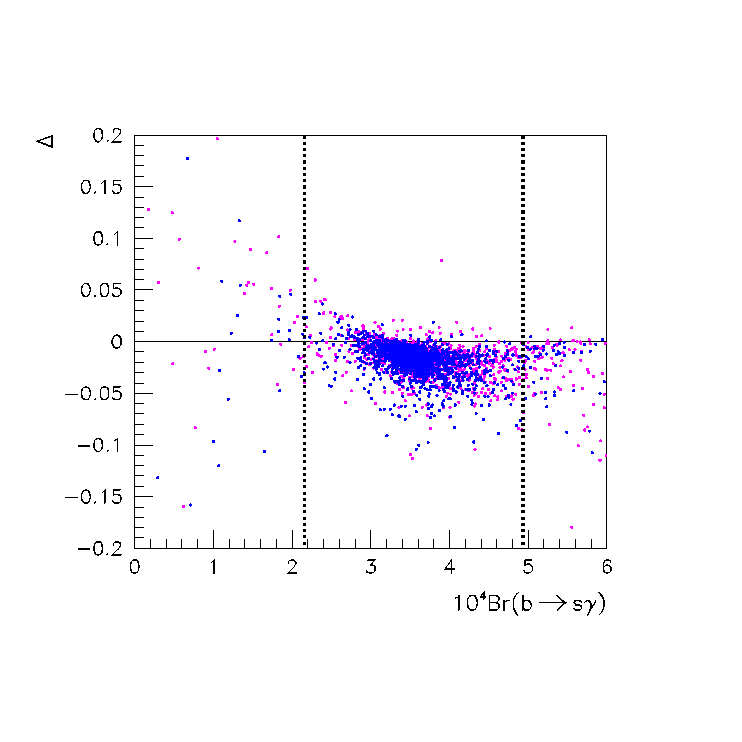
\includegraphics[width=8cm]{bsgiso.eps}
\vspace{-.3cm}
\caption{ Relative difference for $B(\bar{B}\rightarrow s\gamma)$ between micromegas$2.4$ and superIso$3.1$.
the vertical lines show the $3\sigma$ experimentally measured value.
}
\label{fig:iso}

\end{figure}


\bibliography{manual}
\end{document}



The function\\
$\bullet$\verb|darkOmegaInflDecay(|$H_I$,$\Gamma$, Beps,\&$a_{end}$,\&Trh,\&isWIMP, \&err)\\
calculates the DM relic density taking into account the entropy injection from inflaton decay \cite{Gelmini:2006pw}. Here $H_I$ is the  Hubble rate caused by initial  inflaton density, $\Gamma$ is the width of inflaton. 
% and the return parameter $a_{end}$ 
%is  a scale factor for the expansion  of the Universe from the  end of inflation until the  temperature {\tt Tend} is reached. 

We consider two equations for $z_s= s^{4/3} a^4$ and  
 $z_\phi= \rho_\phi a^3$
\begin{eqnarray} 
\label{Infl_evol_s} 
   \frac{dz_s}{da}&=&\frac{4}{3}\frac{\Gamma}{H}  \frac{s^{1/3}}{T} z_\phi \\
\label{Infl_evol_rho} 
   \frac{dz_\phi}{da}&=& -\frac{\Gamma}{H a} z_\phi 
\end{eqnarray}
where
 \begin{equation}
 H^2=\frac{8\pi}{3 M_P^2}\left( \rho_\phi+\frac{\pi^2}{30} g_{eff}(T)T^4\right),
\end{equation}
 $\rho_\phi$ is the mass density of inflatons and $M_P$ the Planck mass. The  
 temperature $T$ is obtained by solving the equation for the  entropy density of the SM bath,  $s$ ,
\begin{equation} 
    s=\frac{2\pi^2}{45} h_{eff}(T) T^3.
\end{equation} 
The initial inflaton density is 
\begin{equation}
   \rho_\phi=\left( \frac{3}{8\pi} H_I M_P\right)^2
\end{equation} 
The solution of Eqs.~\ref{Infl_evol_s}, \ref{Infl_evol_rho} is stored into the tabulated functions {\tt Ta(a)} and {\tt Ha(a)} which respectively return the  temperature and Hubble parameter as  function of the scale parameter $a \in [1,a_{end}]$. These functions are available to the user. Then the code solves the evolution equation for the DM number density 
\begin{equation} 
 \label{Infl_evol_dm} 
 \frac{dz_{DM}}{da}= -\frac{1}{ H a^4}\left( \langle v\sigma_A\rangle \left( z_{DM}^2 -\bar{z}_{DM}^2\right)+\langle v\sigma_S\rangle \left(z_{DM}^2-z_{DM} \bar{z}_{DM}\right)  \right)
\end{equation}
 where  $z_{DM} = n_{DM} a^3$ and $\bar{z}_{DM}=\bar{n}_{DM} a^3$ with $n_{DM}$  the  DM number density and  $\bar{n}_{DM}$  the equilibrium DM number density.   
Before solving  Eq.\ref{Infl_evol_dm} the code tries  to find a low temperature region, where the  DM is in thermal  equilibrium with the SM bath. We use the following conditions of equilibrium 
\begin{eqnarray}
  | \delta z| &<& 10^{-2} \bar{z}_{DM}\\
   \delta a/a &<& 10^{-3}
\end{eqnarray}
where $\delta z $ and $\delta a$ are estimations of the deviation from equilibrium and  for the step of integration
\begin{eqnarray}
   \delta z &=& -\frac{ d log(\bar{z}_{DM}) }{ d a} \frac{H a^4}{ 2<v\sigma_A>_T +  <v\sigma_S>_T  }\\
   \delta a &=&  \frac{ H a^4}{ \bar{z}_{DM} ( 2<v\sigma_A>_T +  <v\sigma_S>_T)} 
\end{eqnarray}   
 If the conditions for thermal equilibrium are satisfied, the integration starts from the largest scale parameter $a$ where the equilibrium condition holds and the  initial value is taken to be $z_{DM}=\bar{z}_{DM}+ \delta z$. Otherwise the  integration starts from $a=1$ with zero initial conditions.
   

The main return value of this routine is the DM relic density  $\Omega_{DM}h^2$. The  auxiliary  output parameters are  {\it double} $a_{end}$,  { \it double}  {\tt Trh}, {\it integer} {\tt isWIMP}, and {\it integer} {\tt err}. 
$a_{end}$ is  a scale factor for the expansion  of the Universe from the  end of inflation until the  temperature {\tt Tend}  is reached.
%presents a factor of expansion  for temperature {\tt Tend}, where the program  stops evolution. 
 {\tt Trh} is the reheating temperature, it is defined as the temperature at which the inflaton and the SM bath give the same contribution to the  Hubble rate.
The parameter {\tt isWIMP} indicates whether  or not the DM candidate behaves as  a WIMP, namely  if the final relic density decreases when the cross section increases, then  {\tt isWIMP=1}, otherwise {\tt isWIMP=0}.   The error code {\tt err}  indicates whether there is  a problem with  the  solution of the differential equations 
\ref{Infl_evol_s}, \ref{Infl_evol_rho}, in which case the 8-th bit of the error code {\tt err} is 1, or with  the solution of  Eq.\ref{Infl_evol_dm}, then  the 9-th bit is 1. The lowest bits contain information about problems with numerical integration and should be treated as warnings.

The evolution of  the DM abundance is  stored in an  array and is  available  via the functions {\tt Za(a)}, {\tt ZaEq(a)}, \verb|Ya(a)|\footnote{ The function {\tt YaEq(a)} can be constructed as {\tt Yeq(Ta(a)}}  defined in the interval $ a \in
[1,a_{end}]$. 


\begin{tabular}{|l|l|l|l|}
\hline
 textual label &  dimension       &  array of data               & array of error     \\
                  \cline{3-4}            
               &                  &  array of data               &  NULL              \\
                  \cline{2-4}
                &   0             & {\it (double* f)(double x)}   &  NULL              \\
                  \cline{3-4} 
                &                & {\it (double* f)(double x, void*arg)}&  arg       \\
\hline    
\end{tabular}\\
